This chapter provides a detailed overview of all the hardware components of the Single Chip Mote digital system. The Single Chip Mote hardware encompasses all of the Verilog files, Verilog header files, and ISE project files used to describe the Single Chip Mote digital system. The intention of this chapter is to provide clarification and guidance to those planning on reading or modifying the hardware, and its is highly recommended that this chapter be read alongside the Verilog code described in each section. This chapter may also provide some useful insight for software developers designing applications for the Single Chip Mote, in particular the sections on register interfaces.

Some of the files and designs described in this chapter are provided by ARM with the Cortex-M0 DesignStart kit (see section \ref{arm-ds} for more information), such as the Verilog for the Cortex-M0 and AHB controllers for various peripherals on the Nexys 3 board. There are also Verilog modules designed by Francesco Bigazzi, a visiting scholar who originally worked on the Single Chip Mote digital system, such as the bridge between AHB and APB, and some of the APB peripherals. All other work described in this section not attributed to ARM, Bigazzi, or any other designer is original. 

\section{ISE Project Settings} \label{ise-project-settings}
ISE projects have already been created for the Single Chip Mote digital system on the Artix-7 and Spartan-6, as well as the bootload hardware (chapter \ref{bootloading}) for the Spartan-6. However, it may be necessary in the future to make more ISE projects for additional FPGA designs, such as running the bootload hardware (chapter \ref{bootloading}) on the Artix-7. This section contains the information needed to create a new project for the versions of these chips running on the Nexys 4 DDR and Nexys 3 boards.

\subsection{Artix-7}
In order to create a new ISE project for the Artix-7 FPGA on the Nexys 4 DDR board, open ISE and choose New Project in the File menu. In the New Project Wizard window, enter a name for the project and specify the location of the project files. It is suggested that all project files related to Single Chip Mote be checked into the repo in \path{scm-digital/proj/ise/artix7/}. After selecting Next, the New Project Wizard will display the options for the device and design flow for the project. Figure \ref{fig:artix7-project-properties} shows all of the appropriate options for the Artix-7 on the Nexys 4 DDR. Select Next and then Finish to create the new project.

\begin{figure}
	\centering
	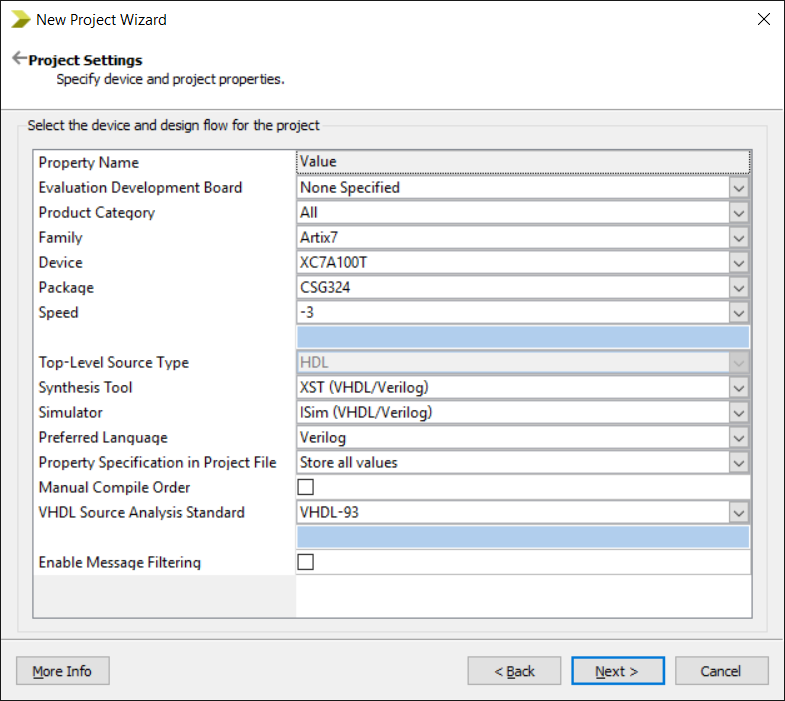
\includegraphics[width=0.7\linewidth]{artix7-project-properties}
	\caption{Project settings used to create a new ISE project for the Artix-7 FPGA on the Nexys 4 DDR}
	\label{fig:artix7-project-properties}
\end{figure}

From here, add any pre-written Verilog files using the Add Source... option in the Project menu. Use the New Source... option in the Project menu to create new source files including Verilog files. All of the project source files will appear in the Design Hierarchy panel. Once the top Verilog module is added or created, select that module in the Design Hierarchy panel and go to the Source menu and select Set as Top Module. Now when this module is selected in the Design Hierarchy Panel, all of the synthesis and other compilation options will appear in the Processes panel.

\subsection{Spartan-6}
In order to create a new ISE project for the Spartan-6 FPGA on the Nexys 3 board, open ISE and choose New Project in the File menu. In the New Project Wizard window, enter a name for the project and specify the location of the project files. It is suggested that all project files related to Single Chip Mote be checked into the repo in \path{scm-digital/proj/ise/spartan6/}. After selecting Next, the New Project Wizard will display the options for the device and design flow for the project. Figure \ref{fig:spartan6-project-properties} shows all of the appropriate options for the Spartan-6 on the Nexys 3. Select Next and then Finish to create the new project.

\begin{figure}
\centering
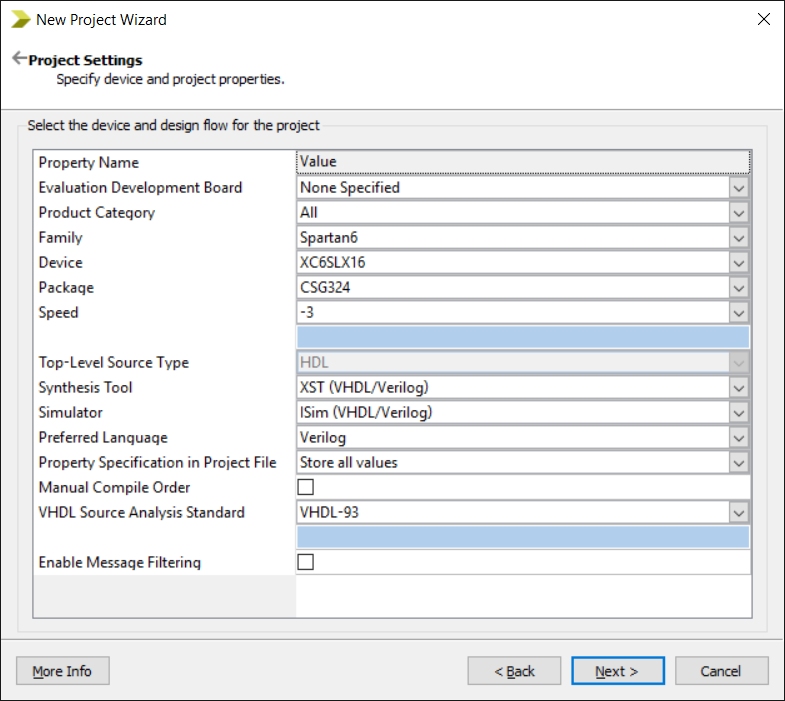
\includegraphics[width=0.7\linewidth]{spartan6-project-properties}
\caption{Project settings used to create a new ISE project for the Spartan-6 FPGA on the Nexys 3}
\label{fig:spartan6-project-properties}
\end{figure}

From here, add any pre-written Verilog files using the Add Source... option in the Project menu. Use the New Source... option in the Project menu to create new source files including Verilog files. All of the project source files will appear in the Design Hierarchy panel. Once the top Verilog module is added or created, select that module in the Design Hierarchy panel and go to the Source menu and select Set as Top Module. When this module is selected in the Design Hierarchy Panel again, all of the synthesis and other compilation options will appear in the Processes panel.

\subsection{User Constraints File}
All ISE projects require a User Constrains File (UCF) in order to map the top module's IOs to the pins on the FPGA package. Given that the FPGAs are soldered onto boards designed by Digilent, not all of the available pins on the package are routed to pins accessible on the Digilent boards. While generic UCF files for the Spartan-6 and Artix-7 FPGAs exist (or are generated using Xilinx tools), Digilent provides master UCF files for their Nexys 3 and Nexys 4 DDR boards listing only the pins that are accessible through one of the various connectors on the boards. These UCF files provide net names and descriptions in the comments of each line to describe how each of the actual FPGA pins map to a physical connector on the board. Digilent also publishes the schematics of their boards, containing the same information as the UCF file comments in a visual form. It is recommended that a clean UCF file is downloaded from Digilent's resource center for every project, and added in ISE using the Add Source... option in the Project menu.

Figure \ref{lst:ucf} contains an excerpt of the UCF file used for the Single Chip Mote digital system on the Nexys 4 DDR. The file is a modified version of the UCF file provided by Digilent for any Nexys 4 DDR design. All of the lines beginning with a hash symbol (\#) are comments. A UCF file must only include pins on the FPGA that are currently in use. All unused pins must be either omitted from the file, or as seen in the example, commented-out.

The top line in Figure \ref{lst:ucf} contains the definition of the \texttt{CLK} net used for the 100MHz input clock. Underneath is a series of lines designating this net as a clock, and specifying its properties such as frequency and duty cycle.

Each input or output is described using a line beginning with \texttt{NET}. This is then followed by the net name, in quotes. The net name corresponds to the name of the input or output in the top module. Input and output buses require that each signal in the bus have its own NET in the UCF file, with the index indicated using angle brackets (\textlangle\textrangle) instead of square brackets ([]).

The location of the pin connected to the net is specified after the net name, using \texttt{LOC=J15}, where J15 is a particular pin on the FPGA. In the case of the Nexys 4 DDR, the pin J15 is connected to one of the switches, hence why this net is included in the Switches section of the provided UCF. The original name of this net was \texttt{sw\textlangle0\textrangle} to indicate that it was connected to the first switch on the board. This is why it is recommended that the UCF files provided by Digilent are used. However, net names must be changed to match the top module (or vice versa) when using the UCF file provided by Digilent.

The \texttt{IOSTANDARD=LVCMOSS33} is an optional attribute, used to specify the attributes for the pin such as voltage, drive, and slew. It is recommended that the default IOSTANDARD specified in the Digilent UCF file is used and not changed unless the proper Xilinx documentation is first consulted.

The comments after each line indicate the name of the pin on the Artix-7 package. The name also contains information on how the pin may be used. For example, all pins with \texttt{MRCC} or \texttt{SRCC} in the name can be used as an input for clock signals. However, if the clock is single-ended, then the pin must also have a P in the second part of the name, for example \texttt{IO\_L13P\_T2\_MRCC\_15}. Differential clock inputs require P/N pairs. The \texttt{IO\_L13P\_T2\_MRCC\_15} pin is the only pin of its kind that is accessible through one of the Pmod connectors on the Nexys 4 DDR board, and therefore this single pin is used for both the input clock for the radio (see section \ref{rfcontroller} for more information) and the input clock for the 3 Wire Bus (see section \ref{3wb} for more details).

\begin{figure}
\begin{lstlisting}
NET "CLK"   LOC = "E3"	|IOSTANDARD = "LVCMOS33";	#Bank = 35, Pin name = #IO_L12P_T1_MRCC_35,	Sch name = clk100mhz
NET "CLK" TNM_NET = sys_clk_pin;
TIMESPEC TS_sys_clk_pin = PERIOD sys_clk_pin 100 MHz HIGH 50%; 

## Switches
NET "gp_in<0>" LOC=J15 |IOSTANDARD=LVCMOS33; #IO_L24N_T3_RS0_15
NET "gp_in<1>" LOC=L16 |IOSTANDARD=LVCMOS33; #IO_L3N_T0_DQS_EMCCLK_14
NET "gp_in<2>" LOC=M13 |IOSTANDARD=LVCMOS33; #IO_L6N_T0_D08_VREF_14
NET "gp_in<3>" LOC=R15 |IOSTANDARD=LVCMOS33; #IO_L13N_T2_MRCC_14
#NET "sw<4>"   LOC=R17 |IOSTANDARD=LVCMOS33; #IO_L12N_T1_MRCC_14
#NET "sw<5>"   LOC=T18 |IOSTANDARD=LVCMOS33; #IO_L7N_T1_D10_14
#NET "sw<6>"   LOC=U18 |IOSTANDARD=LVCMOS33; #IO_L17N_T2_A13_D29_14
#NET "sw<7>"   LOC=R13 |IOSTANDARD=LVCMOS33; #IO_L5N_T0_D07_14
...
## Buttons
NET "RESETn"   LOC=C12 |IOSTANDARD=LVCMOS33; #IO_L3P_T0_DQS_AD1P_15
#NET "btnc"    LOC=N17 | IOSTANDARD=LVCMOS33; #IO_L9P_T1_DQS_14
#NET "btnd"    LOC=P18 | IOSTANDARD=LVCMOS33; #IO_L9N_T1_DQS_D13_14
#NET "btnl"    LOC=P17 | IOSTANDARD=LVCMOS33; #IO_L12P_T1_MRCC_14
#NET "btnr"    LOC=M17 | IOSTANDARD=LVCMOS33; #IO_L10N_T1_D15_14
#NET "btnu"    LOC=M18 | IOSTANDARD=LVCMOS33; #IO_L4N_T0_D05_14
...
## Pmod Header JB
NET "data_3wb"  LOC=D14 |IOSTANDARD=LVCMOS33; #IO_L1P_T0_AD0P_15
NET "latch_3wb" LOC=F16 |IOSTANDARD=LVCMOS33; #IO_L14N_T2_SRCC_15
#NET "jb<3>"    LOC=G16 |IOSTANDARD=LVCMOS33; #IO_L13N_T2_MRCC_15
#NET "jb<4>"    LOC=H14 |IOSTANDARD=LVCMOS33; #IO_L15P_T2_DQS_15
NET "tx_clk"    LOC=E16 |IOSTANDARD=LVCMOS33; #IO_L11N_T1_SRCC_15
NET "tx_dout"   LOC=F13 |IOSTANDARD=LVCMOS33; #IO_L5P_T0_AD9P_15
NET "rx_din"    LOC=G13 |IOSTANDARD=LVCMOS33; #IO_0_15
NET "rx_clk"    LOC=H16 |IOSTANDARD=LVCMOS33; #IO_L13P_T2_MRCC_15
\end{lstlisting}
\caption{An example of a UCF file for the Artix-7 on the Nexys 4 DDR board}
\label{lst:ucf}
\end{figure}

\section{Digital System Architecture Overview}
Figure \ref{fig:system-architecture} contains a block diagram of the top module of the Single Chip Mote digital system, \texttt{uCONTROLLER}, along withs its inputs and outputs to/from the other parts of the Single Chip Mote, such as the analog/RF circuits. The Single Chip Mote digital system consists of one ARM Cortex-M0 DesignStart processor connected to various peripherals through a hierarchy of buses. These peripherals include instruction and data memory, a radio controller, a radio timer, an ADC controller, a UART transmitter and receiver, analog configuration registers for the radio, and general-purpose digital inputs and outputs.

The \texttt{PON} (short for Power-ON) module contains all of the hardware to generate the clocks and handle resets. This module is only required for the FPGA version of the Single Chip Mote digital system. On an ASIC, it is assumed that an external analog circuit handles the generation of all clock and reset signals.

The AHB-Lite is a 32-bit bus used by the ARM Cortex-M0 to connect to memory and peripherals. The main AHB-Lite bus is composed of two modules, \texttt{AHBDCD} and \texttt{AHBMUX}. An example of these modules is provided in the ARM Cortex-M0 DesignStart kit and is used as the basis for this design. This bus has 1 master, the ARM Cortex-M0 and 5 slaves: the instruction memory (\texttt{AHBIMEM}), another AHB-Lite bus (through the arbiter \texttt{AHBLiteArbiter\_V2}), the direct memory access controller (\texttt{DMA\_V2}), the radio timer (\texttt{RFTIMER}), and an APB bus. The second AHB-Lite bus is designed to have two masters (using the \texttt{AHBLiteArbiter\_V2} module as an arbiter) and two slaves, the data memory (\texttt{AHBDMEM}) and the radio controller (\texttt{RFcontroller}). This structure was chosen because the two slaves need to be accessed by both the Cortex-M0 and the DMA. The DMA is used to automatically transfer radio packet data between the radio controller and the data memory without any intervention from the Cortex-M0. The first AHB-Lite bus is referred to as the AHB. The second AHB-Lite bus is referred to as the AHBsub.

The APB is a 16-bit peripheral bus used to access peripherals that do not require the full 32-bit data size or the low latency of the AHB-Lite. The APB is connected to the AHB-Lite using the \texttt{AHB2APB} module designed by Bigazzi. The bus itself is composed of the \texttt{APBMUX} module designed by Bigazzi. This bus has four slaves: the ADC controller (\texttt{APBADC\_V2}), the UART transmitter/receiver (\texttt{APBUART}), configuration registers for the analog circuits of the Single Chip Mote (\texttt{APB\_ANALOG\_CFG}), and a small set of digital inputs and outputs (\texttt{APBGPIO}).

For more information on the AHB-Lite protocol, the APB protocol, and each of the modules mentioned above, see the rest of this chapter.

\begin{figure}
\centerline{
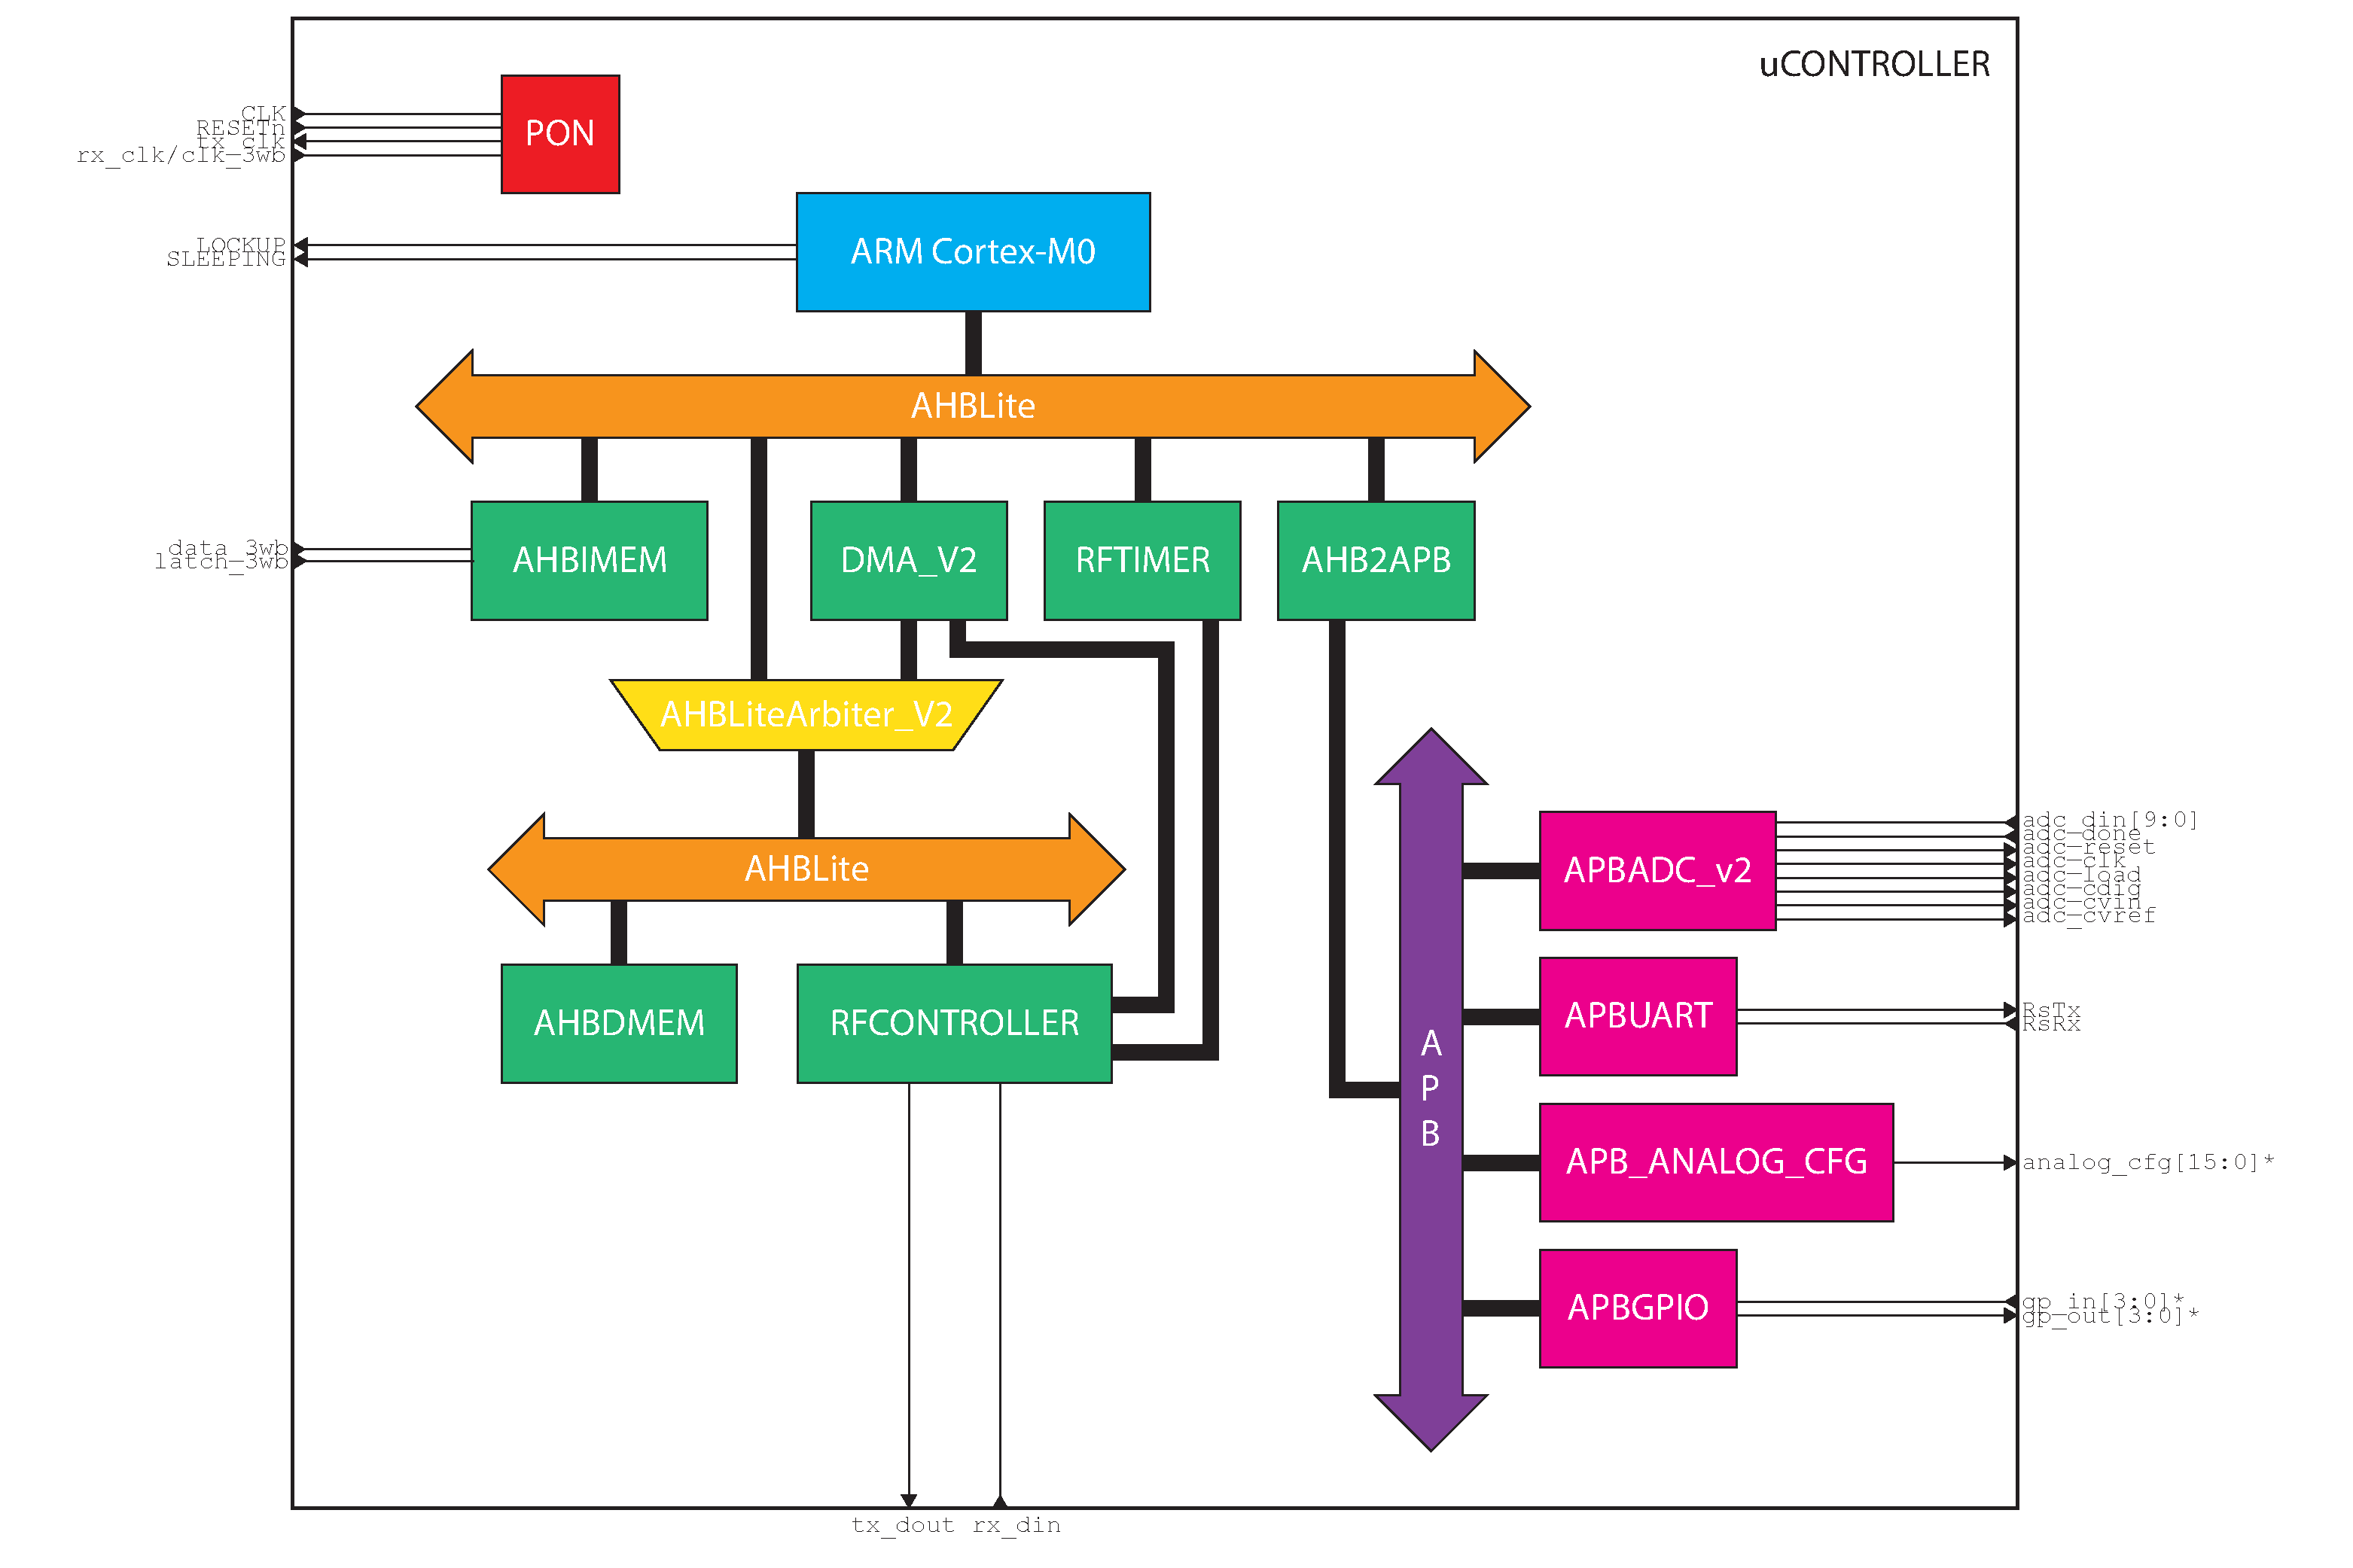
\includegraphics[width=1.25\linewidth]{system-architecture}	
}
\caption{Block diagram of the Single Chip Mote digital system. Inputs/outputs with a * have parameterizable bus widths.}
\label{fig:system-architecture}
\end{figure}

\section{ARM Cortex-M0 Memory Map Specification} \label{memory-map-spec}
The AHB-Lite bus on the ARM Cortex-M0 allows for the use of 4GB addressable memory with 32-bit addresses. In ARM documentation this addressable memory is referred to as the memory map. This does not mean that all Cortex-M0 designs contain at least 4GB of memory storage; instead, all Cortex-M0 designs have 4GB of address space used to access either actual memory or memory-mapped peripherals. 

Each address refers to a single byte in the memory; however, in certain regions of the memory map, the ARM Cortex-M0 DesignStart processor only allows word-aligned accesses. Overall, it is recommended that all memory-mapped peripherals used word-aligned addresses. In this case, the only valid addresses are multiples of 4, such as \texttt{0x0101010C} or \texttt{0xABCDEF08}.

Continuous regions of this address space are reserved for instruction memory, data memory, debug access, and peripherals. Addresses are divided into these regions based on the upper bits of the address. In the Single Chip Mote digital system, the 8 upper bits (referred to in this document as the address prefix) are used to distinguish between memory regions or memory-mapped peripherals. One notable exception is the Private Peripheral Bus, with a 12-bit prefix of \texttt{0xE00}.

Figure \ref{table:memory-map} contains a summary of the memory map for the ARM Cortex-M0. Not all regions of this memory map are currently used in the Single Chip Mote digital system, such as the external data memory or the external device memory.

\begin{figure}
	\centering
	\small
	\centerline{
	\begin{tabular}{|l|l|l|l|}
		\hline
		Address Range & Address Prefix & Memory Region & Description\\
		\hline
		\texttt{0x00000000-} & \texttt{0x00-0x1F} & Code & Executable region for instruction memory.\\
		\texttt{0x1FFFFFFF} & & & This can be ROM, RAM, or both.\\
		 & & & Data can also go here.\\
		\hline
		\texttt{0x20000000-} & \texttt{0x20-0x3F} & SRAM & Executable region for data memory.\\
		\texttt{0x3FFFFFFF} & & & Instructions can also go here.\\
		\hline
		\texttt{0x40000000-} & \texttt{0x40-0x5F} & Peripheral & External device memory. This memory\\
		\texttt{0x5FFFFFFF} & & & is not executable.\\
		\hline
		\texttt{0x60000000-} & \texttt{0x60-0x9F} & External RAM & Executable region for external data\\
		\texttt{0x9FFFFFFF} & & & memory.\\
		\hline
		\texttt{0xA0000000-} & \texttt{0xA0-0xDF} & External Device & Non-executable region for external device\\
		\texttt{0xDFFFFFFF} & & & memory.\\
		\hline
		\texttt{0xE0000000-} & \texttt{0xE00} & Private Peripheral & Non-executable region including special\\
		\texttt{0xE00FFFFF} & & Bus & Cortex-M0 registers such as the NVIC,\\
		 & & & system timer, and system control block.\\
		\hline
		\texttt{0xE0100000}- & \texttt{0xE01-0xFFF} & Device & Implementation-specific device memory.\\
		\texttt{0xFFFFFFFF} & & & This region is reserved for additional ARM\\
		 & & & Cortex-M0 features not available on the\\
		 & & & DesignStart processor.\\
		\hline
	\end{tabular}
	}
	\caption{Memory map of the ARM Cortex-M0}
	\label{table:memory-map}
\end{figure}

For more information on the ARM Cortex-M0 memory map see the Cortex-M0 Devices Generic User Guide \cite{cortex-m0-generic-ug}. A copy is also found in \path{scm-digital/doc/}.

\section{AMBA 3 AHB-Lite Protocol}
This section summarizes the basics of the AMBA 3 AHB-Lite protocol, including specific details involving the implementation of this bus on the Single Chip Mote digital system.

The AHB-Lite bus is a high-bandwidth single-master bus. All slaves on this bus use the same clock, \texttt{HCLK}, and have the same reset, \texttt{HRESETn}. On the Single Chip Mote digital system, almost all modules use \texttt{HCLK} and \texttt{HRESETn} as well, including APB slaves.

The bus master drives the following signals:

\begin{description}
	\item[\texttt{HADDR[31:0]}] The address bus.
	\item[\texttt{HBURST[2:0]}] Indicates whether the transfer is a single transfer or some kind of burst. The DesignStart processor does not generate any BURST transfers \cite{ahblite-mit}. Therefore, this signal is omitted in the Single Chip Mote digital system.
	\item[\texttt{HMASTLOCK}] Indicates that the current transfer is part of a locked sequence. The DesignStart processor does not generate any locked transfers \cite{ahblite-mit}. Therefore, this signal is omitted in the Single Chip Mote digital system.
	\item[\texttt{HPROT[3:0]}] Protection control signal. This can be ignored by the slave \cite{ahblite-mit}, and is omitted in the Single Chip Mote digital system.
	\item[\texttt{HSIZE[2:0]}] Indicates the size of the transfer as a byte, halfword, or word.
	\item[\texttt{HTRANS[1:0]}] Indicates the transfer type. The DesignStart processor only uses non-sequential transfers \cite{ahblite-mit}, making \texttt{HTRANS[0]} always 0. Therefore, \texttt{HTRANS[0]} is omitted in the Single Chip Mote digital system.
	\item[\texttt{HWDATA[31:0]}] The write data when the master writes to a slave.
	\item[\texttt{HWRITE}] Indicates if the transfer is a read (0) or write (1).
\end{description}

Slaves each drive their own set of the following signals:

\begin{description}
	\item[\texttt{HRDATA[31:0]}] The read data given to the master when it reads from a slave.
	\item[\texttt{HREADYOUT}] Indicates that the transfer is finished. As long as this signal is 0, the master waits until it is 1 before considering the transfer complete.
	\item[\texttt{HRESP}] Used to indicate an error in the transfer. This is not used by any of the slaves in the Single Chip Mote digital system and is omitted.
\end{description}

The \texttt{AHBDCD} module takes the address for the current transfer and selects the correct slave using the address prefix. This module is connected to the \texttt{AHBMUX} module, which selects the correct set of slave signals to send to the master. The \texttt{AHBDCD} module also drives the various \texttt{HSEL} signals to each slave, used to indicate that the transfer is intended for that particular slave.

Each bus transfer requires two phases, the address phase and the data phase. In the address phase, the master sets the \texttt{HADDR}, \texttt{HWRITE}, \texttt{HTRANS}, and other relevant signals. The next cycle is the beginning of the data phase, where the slave sets \texttt{HRDATA} (if the transfer is a read), performs a write (if the transfer is a write) and sets \texttt{HREADYOUT} if the transfer is complete. The slave can stall the master by leaving \texttt{HREADYOUT} low.

This protocol supports pipelined transfers. This means that the data phase of one transfer can also be the address phase of the next transfer. The address phase signals remain constant/valid while the master is stalled during a data phase, and do not change until \texttt{HREADYOUT} from the slave is high.

For more information on the AHB-Lite, see the AMBA 3 AHB-Lite Protocol Specification \cite{ahb-lite-spec}. A copy is also found in \path{scm-digital/doc/}.

\section{AMBA 3 APB Protocol}
This section summarizes the basics of the AMBA 3 APB protocol, including specific details involving the implementation of this bus on the Single Chip Mote digital system.

The APB bus is a low-power reduced-complexity bus for peripherals that do not require high bandwidth or low latency. The protocol defines separate clock (\texttt{PCLK}) and reset (\texttt{PRESETn}) signals for APB slaves. In the Single Chip Mote digital system, \texttt{HCLK} and \texttt{HRESETn} are used instead.

The master of this bus is the composed of the bridge connecting the AHB and APB (the \texttt{AHB2APB} module) and the \texttt{APBMUX} module that indicates which slave is being accessed and sends the correct set of slave signals to the master. The master drives the following signals:

\begin{description}
	\item[\texttt{PADDR[15:0]}] The address bus.
	\item[\texttt{PSEL}] Each slave has one of these signals to indicate that the transfer is intended for that particular slave.
	\item[\texttt{PENABLE}] Indicates the second and subsequent cycles of a transfer.
	\item[\texttt{PWRITE}] Indicates if the transfer is a read (0) or write (1).
	\item[\texttt{PWDATA[15:0]}] The write data when the master writes to a slave.
\end{description}

The slaves each drive their own set of the following signals:

\begin{description}
	\item[\texttt{PREADY}] Indicates that the transfer is finished. As long as this signal is 0, the master waits until it is 1 before considering the transfer complete.
	\item[\texttt{PRDATA[15:0]}] The read data given to the master when it reads from a slave.
	\item[\texttt{PSLVERR}] Indicates a transfer failure. This is optional and is not used by any of the slaves in the Single Chip Mote digital system and is omitted.
\end{description}

Each bus transfer requires two phases, the setup phase and the access phase. The first clock cycle is the setup phase, where \texttt{PADDR}, \texttt{PWDATA}, and \texttt{PWRITE} are set by the master. During the second clock cycle, the \texttt{PENABLE} signal is asserted to indicate that it is now the access phase. All control signals stay the same during the access phase as the APB protocol does not allow for pipelined transfers. The access phase is extended by keeping the \texttt{PREADY} signal low. The transfer completes once \texttt{PREADY} is high.

For more information on the APB, see the AMBA 3 APB Protocol Specification \cite{apb-spec}. A copy is also found in \path{scm-digital/doc/}.

\section{Header Files and Parameters}
The Verilog for the Single Chip Mote digital system contains two header files, \path{SYS_PROP.vh} and \path{REGISTERS.vh}, used parameterize the design and make it easy to modify. 

\subsection{SYS\_PROP.vh}
\path{SYS_PROP.vh} contains \texttt{\`{}define} statements used to tweak module parameters (such as the baud rate for \texttt{APBUART} or the number of outputs in \texttt{APBGPIO}). Each parameterizable module has a parameter defined in the module definition. If a module is not instantiated in the top level, then its parent module defines the same parameter, and passes the value on during instantiation. If there are several submodules between the top level and the module requiring the parameter, then each module in that chain must instantiate the parameter and pass it down. At the top level, the name defined in \path{SYS_PROP.vh} is passed into the module instantiation.

For example, consider the \texttt{compare\_unit} module, with the following definition:
\begin{lstlisting}
module compare_unit(
	...
	...
	...
);

// Parameters
parameter COUNTER_WIDTH = 32;
\end{lstlisting}

This module is instantiated in the \texttt{RFTIMER} module using the following syntax:

\begin{lstlisting}
compare_unit #(.COUNTER_WIDTH(COUNTER_WIDTH)) u_compare_unit (
	...
	...
	...
);
\end{lstlisting}

The \texttt{RFTIMER} module also contains the same parameter, \texttt{COUNTER\_WIDTH}, along with its own parameters:

\begin{lstlisting}
module RFTIMER(
	...
	...
	...
);

// Parameters
parameter NUM_COMPARE_UNITS = 8;
parameter NUM_CAPTURE_UNITS = 4;
parameter COUNTER_WIDTH = 32;
\end{lstlisting}

And \texttt{RFTIMER} is instantiated at the top level, \texttt{uCONTROLLER}, using the values defined in \path{SYS_PROP.vh}:

\begin{lstlisting}
RFTIMER #(
	.NUM_COMPARE_UNITS(`RFTIMER_NUM_COMPARE_UNITS),
	.NUM_CAPTURE_UNITS(`RFTIMER_NUM_CAPTURE_UNITS),
	.COUNTER_WIDTH(`RFTIMER_COUNTER_WIDTH)
) u_RFTIMER (
	...
	...
	...
);
\end{lstlisting}
\begin{lstlisting}
// RFTIMER Specifications
`define RFTIMER_NUM_COMPARE_UNITS   8   // the number of compare units for the timer, if this changes REGISTERS.vh must be updated
`define RFTIMER_NUM_CAPTURE_UNITS   4   // the number of capture units for the timer, if this changes REFISTERS.vh must be updated
`define RFTIMER_COUNTER_WIDTH       32  // the width of the counter for the timer, maximum is 32
\end{lstlisting}

Not all parameters need to be exposed all the way to the top level. For example, state encodings are typically enumerated using parameters. However, these states are specific only to the module itself and are not system-level parameters. Therefore, it is recommended that they are defined as localparams instead of parameters.
 
\subsection{REGISTERS.vh}
\path{REGISTERS.vh} contains \texttt{\`{}define} statements used to assign addresses to peripherals on the AHB and APB and each of their registers. This is first done by assigning an 8-bit address prefix to each peripheral. Then these prefixes are used to define a base address for each peripheral. Then this base address is used to define all register addresses for that peripheral.

As stated in section \ref{memory-map-spec}, all addresses with a prefix in the range of \texttt{0x40-0x5F} can be used for peripheral devices. In the Single Chip Mote digital system, all addresses with a prefix in the range of 
\texttt{0x40-0x4F} are reserved for AHB peripherals, and all addresses with a prefix in the range of \texttt{0x50-0x5F} are reserved for APB peripherals. The only exceptions are the instruction instruction memory (with a prefix of \texttt{0x00}), the bootloader (\texttt{0x01}), and the data memory (\texttt{0x20}), as these are not really system peripherals but are memories used by the ARM Cortex-M0. The first section of \path{REGISTERS.vh} defines these prefixes:

\begin{lstlisting}
// AHB Address Prefixes
`define AHB_PREFIX__IMEM            8'h00
`define AHB_PREFIX__BOOTLOADER      8'h01
`define AHB_PREFIX__DMEM            8'h20
`define AHB_PREFIX__RFCONTROLLER    8'h40
`define AHB_PREFIX__DMA             8'h41
`define AHB_PREFIX__RFTIMER         8'h42
`define AHB_PREFIX__APB             8'b0101_xxxx

// APB Address Prefixes
`define APB_PREFIX__ADC             8'h50
`define APB_PREFIX__UART            8'h51
`define APB_PREFIX__ANALOG_CFG      8'h52
`define APB_PREFIX__GPIO            8'h53
\end{lstlisting}

These prefixes are also used in the \texttt{AHBDCD} and \texttt{APBMUX} modules to determine the AHB/APB signals for each slave based on address.

The next section of \path{REGISTERS.vh} uses these prefixes to define a base address for each peripheral:

\begin{lstlisting}
// AHB Peripheral Base Addresses
`define AHB_BASE__IMEM              { `AHB_PREFIX__IMEM, 24'h00_0000 }
`define AHB_BASE__BOOTLOADER        { `AHB_PREFIX__BOOTLOADER, 24'h00_0000 }
`define AHB_BASE__DMEM              { `AHB_PREFIX__DMEM, 24'h00_0000 }
`define AHB_BASE__RFCONTROLLER      { `AHB_PREFIX__RFCONTROLLER, 24'h00_0000 }
`define AHB_BASE__DMA               { `AHB_PREFIX__DMA, 24'h00_0000 }
`define AHB_BASE__RFTIMER           { `AHB_PREFIX__RFTIMER, 24'h00_0000 }
`define AHB_BASE__APB               { `AHB_PREFIX__APB, 24'h00_0000 }

// APB Peripheral Base Addresses
`define APB_BASE__ADC               { `APB_PREFIX__ADC, 8'h00 }
`define APB_BASE__UART              { `APB_PREFIX__UART, 8'h00 }
`define APB_BASE__ANALOG_CG         { `APB_PREFIX__ANALOG_CFG, 8'h00 }
`define APB_BASE__GPIO              { `APB_PREFIX__GPIO, 8'h00 }
\end{lstlisting}

This base address is the first address in the region of addresses allocated to the peripheral. For example, the \texttt{RFcontroller} module has a prefix of \texttt{0x40} and thus a base address of \texttt{0x40000000}. All register addresses are described relative to an offset from the base. Any changes in the prefix automatically change the base address and all register addresses for that peripheral. Note that the APB uses 16-bit addresses instead of 32-bit addresses.

The last section of \path{REGISTERS.vh} uses the base addresses to define all of the register addresses for the AHB/APB peripherals:

\begin{lstlisting}
// RF Controller
`define RFCONTROLLER_REG__CONTROL           `AHB_BASE__RFCONTROLLER + 32'h0000_0000
`define RFCONTROLLER_REG__STATUS            `AHB_BASE__RFCONTROLLER + 32'h0000_0004
`define RFCONTROLLER_REG__TX_DATA_ADDR      `AHB_BASE__RFCONTROLLER + 32'h0000_0008
`define RFCONTROLLER_REG__TX_PACK_LEN       `AHB_BASE__RFCONTROLLER + 32'h0000_000C
...

// GPIO
`define APBGPIO_REG__INPUT          `APB_BASE__GPIO         + 16'h0000
`define APBGPIO_REG__OUTPUT         `APB_BASE__GPIO         + 16'h0004

\end{lstlisting}

These address definitions are used in any Verilog code that refers to specific register addresses or prefixes. Using define statements for each address ensures that they are easily accessible in one file and all changes propagate to any modules relying on these addresses or prefixes.

The \path{REGISTERS.vh} file could also be parsed by a script to generate a C header file for the purposes of software development. Another option is to define all prefixes and registers in a CSV file, and use a script to create both \path{REGISTERS.vh} and a C header file. Neither of these options are currently implemented, though it is recommended that such a script is created for future work on the Single Chip Mote digital system. % the use of could here is justified

\section{Module Hierarchy}
Figure \ref{verb:module-hierarchy} contains a list of all of the Single Chip Mote digital system modules and their submodules. This list matches the Design Hierarchy panel in ISE Project Navigator.

\begin{figure}
	\small
	\begin{verbatim}
	uCONTROLLER
	    PON
	        pb_debounceRESET
	        ClockDiv
	    CORTEXM0DS
	        cortexm0ds_logic
	    DMA_V2
	    AHBDCD
	    AHBMUX
	    AHBIMEM
	        instruction_ROM
	        instruction_RAM
	    RFTIMER
	        compare_unit
	        capture_unit
	    AHBLiteArbiter_V2
	    AHBDCDsub
	    AHBMUXsub
	    AHBDMEM
	        dmem_ram
	    RFCONTROLLER
	        tx_fifo2
	            tx_fifo_mem
	            tx_rdptr_empty
	            tx_wrptr_full
	            tx_async_comp
	        spreader
	            symbol2chips
	        bit_sync
	        corr_despreader
	            correlator
	        bus_sync
	        rx_fifo
	            rx_fifo_mem
	            rx_rdptr_empty
	            rx_wrptr_full
	            rx_async_comp
	        crcParallel
	    AHB2APB
	    APBMUX
	    APBADC_V2
	    APBUART
	        BAUDGEN
	        FIFO
	        UART_RX
	        UART_TX
	    APB_ANALOG_CFG
	    APBGPIO
	\end{verbatim}
	\caption{Module Hierarchy for the Single Chip Mote digital system}
	\label{verb:module-hierarchy}
\end{figure}

\section{uCONTROLLER}

\subsection{Description}
\texttt{uCONTRLLER} (found in \path{TOP_SYS.v}) is the top module of the Single Chip Mote digital system. This module instantiates the Cortex-M0, power-on moudle, the AHB/APB peripherals, and the AHB/APB busses. This module also connects the above mentioned modules together and to the main inputs and outputs of the Single Chip Mote digital system.

\subsection{Input/Output Ports}
\begin{description}
	\item[\texttt{CLK}] 100MHz clock input from the FPGA board.
	\item[\texttt{RESETn}] Reset input from a button on the FPGA board.
	\item[\texttt{LOCKUP}] Output to an LED on the FPGA board, connected to the LOCKUP output from \texttt{CORTEXM0DS}.
	\item[\texttt{SLEEPING}] Output to an LED on the FPGA board, connected to the SLEEPING output from \texttt{CORTEXM0DS}.
	\item[\texttt{RsRx}] Receive data input for UART.
	\item[\texttt{RsTx}] Transmit data output for UART.
	\item[\texttt{adc\_din[9:0]}] Data input from the ADC.
	\item[\texttt{adc\_done}] Done input from the ADC.
	\item[\texttt{adc\_reset}] Reset output to the ADC.
	\item[\texttt{adc\_clk}] Clock output to the ADC.
	\item[\texttt{adc\_load}] Load output to the ADC.
	\item[\texttt{adc\_cdig}] Cdig output to the ADC.
	\item[\texttt{adc\_cvin}] Cvin output to the ADC.
	\item[\texttt{adc\_cvref}] Cvref output to the ADC.
	\item[\texttt{analog\_cfg[(\`{}ANALOGCFG\_NUM\_REG*16)-1:0]}] Analog configuration outputs to the rest of the Single Chip Mote system. The size of this port depends on the number of 16-bit analog configuration registers in the \texttt{APB\_ANALOG\_CFG} module.
	\item[\texttt{gp\_in[\`{}GPIO\_NUM\_INPUTS-1:0]}] General-purpose digital inputs. The size of this port depends on the number of general-purpose digital inputs in the \texttt{APBGPIO} module.
	\item[\texttt{gp\_in[\`{}GPIO\_NUM\_OUTPUTS-1:0]}] General-purpose digital outputs. The size of this port depends on the number of general-purpose digital outputs in the \texttt{APBGPIO} module.
	\item[\texttt{rx\_clk}] Input clock aligned with the data received from the radio circuit.
	\item[\texttt{rx\_din}] Data input for data received from the radio circuit. On the FPGAs this input is also used as the clock input for the 3 Wire Bus used for bootloading (chapter \ref{bootloading}).
	\item[\texttt{tx\_clk}] Output clock aligned with the data sent to the radio circuit.
	\item[\texttt{tx\_dout}] Data output for data sent to the radio circuit.
	\item[\texttt{data\_3wb}] Data input for the 3 Wire Bus used for bootloading (chapter \ref{bootloading}).
	\item[\texttt{latch\_3wb}] Latch input for the 3 Wire Bus used for bootloading (chapter \ref{bootloading}).
\end{description}

\subsection{Design Details}
\texttt{uCONTROLLER} is the top-level module, used to connect all other modules to one another and to the inputs and outputs of the design as a whole. It contains the instantiations of all the other modules (see Figure \ref{verb:module-hierarchy} for its submodules), and declarations for the wires connecting these modules. Any new buses or peripherals must be instantiated in this module.

\section{CORTEXM0DS}
\subsection{Description}
This module, provided by ARM in the DesignStart kit, is an interface between the obfuscated Verilog describing the ARM Cortex-M0 DesignStart processor (in \texttt{cortexm0ds\_logic}) and the rest of the system.

\subsection{Input/Output Ports}
\begin{description}
	\item[\texttt{HCLK}] Clock input.
	\item[\texttt{HRESETn}] Asynchronous reset input.
	\item[\texttt{HADDR[31:0]}] AHB transfer address output.
	\item[\texttt{HBURST[2:0]}] AHB burst output. This is always 0 and is omitted in the Single Chip Mote digital system.
	\item[\texttt{HMASTLOCK}] AHB locked transfer output. This is always 0 and is omitted in the Single Chip Mote digital system.
	\item[\texttt{HPROT[3:0]}] AHB transfer protection output. AHB slaves do not have to use this signal and therefore it is omitted in the Single Chip Mote digital system.
	\item[\texttt{HSIZE[2:0]}] AHB transfer size output. Indicates a byte, half-word, or word transfer.
	\item[\texttt{HTRANS[1:0]}] AHB transfer type output. This is only set to idle or non-sequential, and therefore \texttt{HTRANS[0]} is always 0. \texttt{HTRANS[0]} is omitted in the Single Chip Mote digital system.
	\item[\texttt{HWDATA[31:0]}] AHB write data output.
	\item[\texttt{HWRITE}] AHB write output. Indicates that the transfer is a write when 1.
	\item[\texttt{HRDATA[31:0]}] AHB read data input.
	\item[\texttt{HREADY}] AHB transfer finished input. This is used to stall the Cortex-M0 when the slave is not finished with the transfer.
	\item[\texttt{HRESP}] AHB error response input. AHB slaves in the Single Chip Mote digital system do not use this signal and therefore it is assigned to 0.
	\item[\texttt{NMI}] Non-maskable interrupt input. This interrupt is not used in the Single Chip Mote digital system and therefore it is assigned to 0.
	\item[\texttt{IRQ[15:0]}] Interrupt request inputs for up to 16 interrupts. Only four are in use right now and the rest are assigned to 0.
	\item[\texttt{TXEV}] Event output. This is not used in the Single Chip Mote digital system.
	\item[\texttt{RXEV}] Event input. This is not used in the Single Chip Mote digital system and is assigned to 0.
	\item[\texttt{LOCKUP}] Lockup output. Indicates that the core is locked-up.
	\item[\texttt{SYSRESETREQ}] System reset request output. Used to send a request for a reset to the \texttt{PON} module.
	\item[\texttt{SLEEPING}] Sleeping output. Indicates that the core and NVIC are sleeping.
\end{description}

\section{cortexm0ds\_logic}
\subsection{Description}
This module, provided by ARM in the DesignStart kit, contains the obfuscated Verilog describing the ARM Cortex-M0 DesignStart processor. This module is instantiated only in \texttt{CORTEXM0DS} and must not be instantiated by any other module in the design. This module must not be modified.

\section{PON} \label{PON}
\subsection{Description}
This module is designed to handle all of the clock and reset signals in the Single Chip Mote digital system. This includes dividing down the 100MHz input clock into all other required clocks, buffering additional clock inputs, debouncing the input reset signal, and listening for reset requests from the Cortex-M0.

\subsection{Input/Output Ports}
\begin{description}
	\item[\texttt{CLK\_100Mz}] 100MHz input clock from the FPGA board.
	\item[\texttt{CLK\_RX\_IN}] External clock input for both receiving radio packets (\texttt{CLK\_RX}, 2MHz) and receiving bootloading data (chapter \ref{bootloading}) over the 3 Wire Bus (\texttt{CLK\_3WB}, 5MHz).
	\item[\texttt{CLK\_RX\_EN}] Clock enable input for the radio receive clock (\texttt{CLK\_RX}). This enable signal is used to ensure that the \texttt{RFcontroller} module only uses the external clock when listening for radio packets.
	\item[\texttt{CLK\_3WB\_EN}] Clock enable input for the 3 Wire Bus clock (\texttt{CLK\_3WB}). This enable signal is used to ensure that the \texttt{AHBIMEM} module only uses the external clock when listening for bootloading data (chapter \ref{bootloading}).
	\item[\texttt{RESETn\_in}] Input reset signal from a button on the FPGA board.
	\item[\texttt{SYSRESETREQ}] Reset request input from the Cortex-M0.
	\item[\texttt{CLK\_5MHz}] 5MHz clock output used by most of the Single Chip Mote digital system. This is assigned at the top level to \texttt{HCLK}.
	\item[\texttt{CLK\_TX}] 2MHz output clock used by the \texttt{RFcontroller} module to send radio packets. This is assigned at the top level to \texttt{CLK\_TX}.
	\item[\texttt{CLK\_TX\_OUT}] 2MHz clock output. The output is a copy of \texttt{CLK\_TX} routed to an output on FPGA. This output is used by the radio circuit to send packets. This is assigned at the top level to the \texttt{tx\_clk} output pin.
	\item[\texttt{CLK\_RX}] 2MHz clock output used by the \texttt{RFcontroller} module to listen for radio packets. This is a buffered version of the \texttt{CLK\_RX\_IN} input clock, enabled or disabled with the \texttt{CLK\_RX\_EN} input. This is assigned at the top level to \texttt{CLK\_RX}.
	\item[\texttt{CLK\_3WB}] 5MHz clock output used by the \texttt{AHBIMEM} module to listen for bootloading data (chapter \ref{bootloading}). This is a buffered version of the \texttt{CLK\_RX\_IN} input clock, enabled or disabled with the \texttt{CLK\_3WB\_EN} input. This is assigned at the top level to \texttt{CLK\_3WB}.
	\item[\texttt{CLK\_RFTIMER}] 500kHz clock output used by the \texttt{RFTIMER} module for its timer. This is assigned at the top level to \texttt{CLK\_RFTIMER}.
	\item[\texttt{HARD\_RESETn\_out}] Hard reset output. The hard reset is active-low. This reset is activated when the external reset button is pressed and not when \texttt{SYSRESETREQ} is asserted. This hard reset is only used in the \texttt{AHBIMEM} module for bootloading purposes (chapter \ref{bootloading}). This is assigned at the top level to \texttt{HARD\_RESETn}.
	\item[\texttt{SOFT\_RESETn\_out}] Soft reset output. This soft reset is active-low. This reset is activated when either the external reset button is pressed or when \texttt{SYSRESETREQ} is asserted. This soft reset is used by every module in the Single Chip Mote digital system. This is assigned at the top level to \texttt{HRESETn}.
\end{description}

\subsection{Design Details}
On an FPGA this module instantiates special primitives used to deal with buffering input clocks, dividing input clocks, attaching derived clocks to the FPGA's clock nets, and buffering any output clocks. See Xilinx documentation for more information on how to use the primitives mentioned in this section. This module uses the \texttt{pb\_debounceRESET} module written by Bigazzi, to debounce the input reset signal. This module also uses the \texttt{ClockDiv} module written by Bigazzi to divide the 100MHz clock into slower clocks that cannot be achieved using FPGA primitives. Note that there are slight differences in the available FPGA primitives on the Artix-7 and Spartan-6.

\subsubsection{Input Clock Buffering}
Both the Artix-7 and Spartan-6 versions of the \texttt{PON} module use the \texttt{IBUFG} primitive to buffer input clocks. This is required whenever a clock is fed into the FPGA from outside. There is an instantiated \texttt{IBUFG} module for both \texttt{CLK\_100MHz} and \texttt{CLK\_RX}.

\subsubsection{Clock Division}
The Artix-7 and Spartan-6 FPGAs use separate primitives for clock division. The Artix-7 version of this module uses \texttt{MMCME2\_ADV} and the Spartan-6 version uses \texttt{DCM\_SP}. On both FPGAs these primitives have a limited range of division. With a 100MHz input clock, the lowest possible frequency is 2.5MHz. Therefore these primitives are only used to divide the 100MHz input to 5MHz for \texttt{CLK\_5MHz}. All slower clocks, such as \texttt{CLK\_TX} at 2MHz, and \texttt{CLK\_RFTIMER} at 500kHz, use the \texttt{ClockDiv} module.

While Xilinx provides documentation on how to instantiate the primitives for clock division, it is not recommended that this be done manually. Instead, it is better to use the Clocking Wizard in CORE Generator to create a core that meets the required specifications (in this case to divide 100MHz to 5MHz). Once the core is been created and added to the project, running the View HDL Functional Model process (see Figure \ref{fig:clock-coregen}) generates the Verilog code for instantiating all of the required clocking primitives. The code in \texttt{PON} was created by copying the generated code and adding the additional input clocks and clock dividers.

The \texttt{ClockDiv} module is a counter-based clock divider with an output that inverts after a maximum count is reached. Therefore, the output clock period is $ T_{out} = 2 \times MAX\_COUNT \times T_{in} $. This method of clock division is not recommended on FPGAs; however, this method is the only way to generate clocks less than 2.5MHz, and therefore is used for \texttt{CLK\_TX} and \texttt{CLK\_RFTIMER}.

\subsubsection{Derived Clock Buffering}
After the input clocks have been divided, using either primitives or \texttt{ClockDiv}, the derived clocks must be attached to a clock buffer in order to route the clocks on the dedicated clock nets within the FPGAs. Any input clocks that are not divided, such as \texttt{CLK\_RX\_IN}, must also be attached to a clock buffer directly from the input clock buffer primitive. This is done using either the \texttt{BUFG} or \texttt{BUFGCE} primitives. The \texttt{BUFG} primitive is used for continuously running clocks such as \texttt{CLK\_5MHz}, \texttt{CLK\_TX}, and \texttt{CLK\_RFTIMER}. The \texttt{BUFGCE} primitive is used for all clocks requiring an enable signal such as \texttt{CLK\_RX} and \texttt{CLK\_3WB}.

\subsubsection{Output Clock Buffering}
Any clocks sent to an output pin on the FPGA must first be routed to an the input of an output buffer through a method called clock forwarding. On the Artix-7, clock forwarding is accomplished by first feeding the clock into an \texttt{ODDR} primitive, and then feeding the output of that into an \texttt{OBUF} primitive. On the Spartan-6, the \texttt{ODDR2} primitive is used instead of the \texttt{ODDR}.

\subsubsection{Resets}
The \texttt{pb\_debounceRESET} module is designed by Bigazzi to debounce the input reset signal before sending it to the rest of the Single Chip Mote digital system. This is necessary because pressing buttons on the FPGA board leads to unstable or fluctuating outputs before the signal converges. A simple debouncer waits for the signal to be stable for multiple cycles before changing the output, to remove any glitches. This module also sends out a pulse when the signal is stable. This module is a slightly modified version of the \texttt{pb\_debouce} module provided in the ARM Cortex-M0 DesignStart kit. Bigazzi modified this code such that the output is active-low instead of active-high. The pulse generated when the input is stable is used as the hard reset, \texttt{HARD\_RESETn\_out}.

In order to deal with reset requests from the Cortex-M0, the hard reset signal is also combined with the \texttt{SYSRESETREQ} signal and then clocked into a register (see Figure \ref{fig:resets}). The output of this register is the soft reset, \texttt{SOFT\_RESETn\_out}. The \texttt{SYSRESETREQ} signal is asynchronous, and must be synchronized outside of the Cortex-M0 before being used for a reset, hence the register. While this does force the soft reset to be 1 cycle behind the hard reset, only one part of the AHBIMEM module uses the hard reset signal instead of the soft reset, and the timing difference is acceptable.

\begin{figure}
\centering
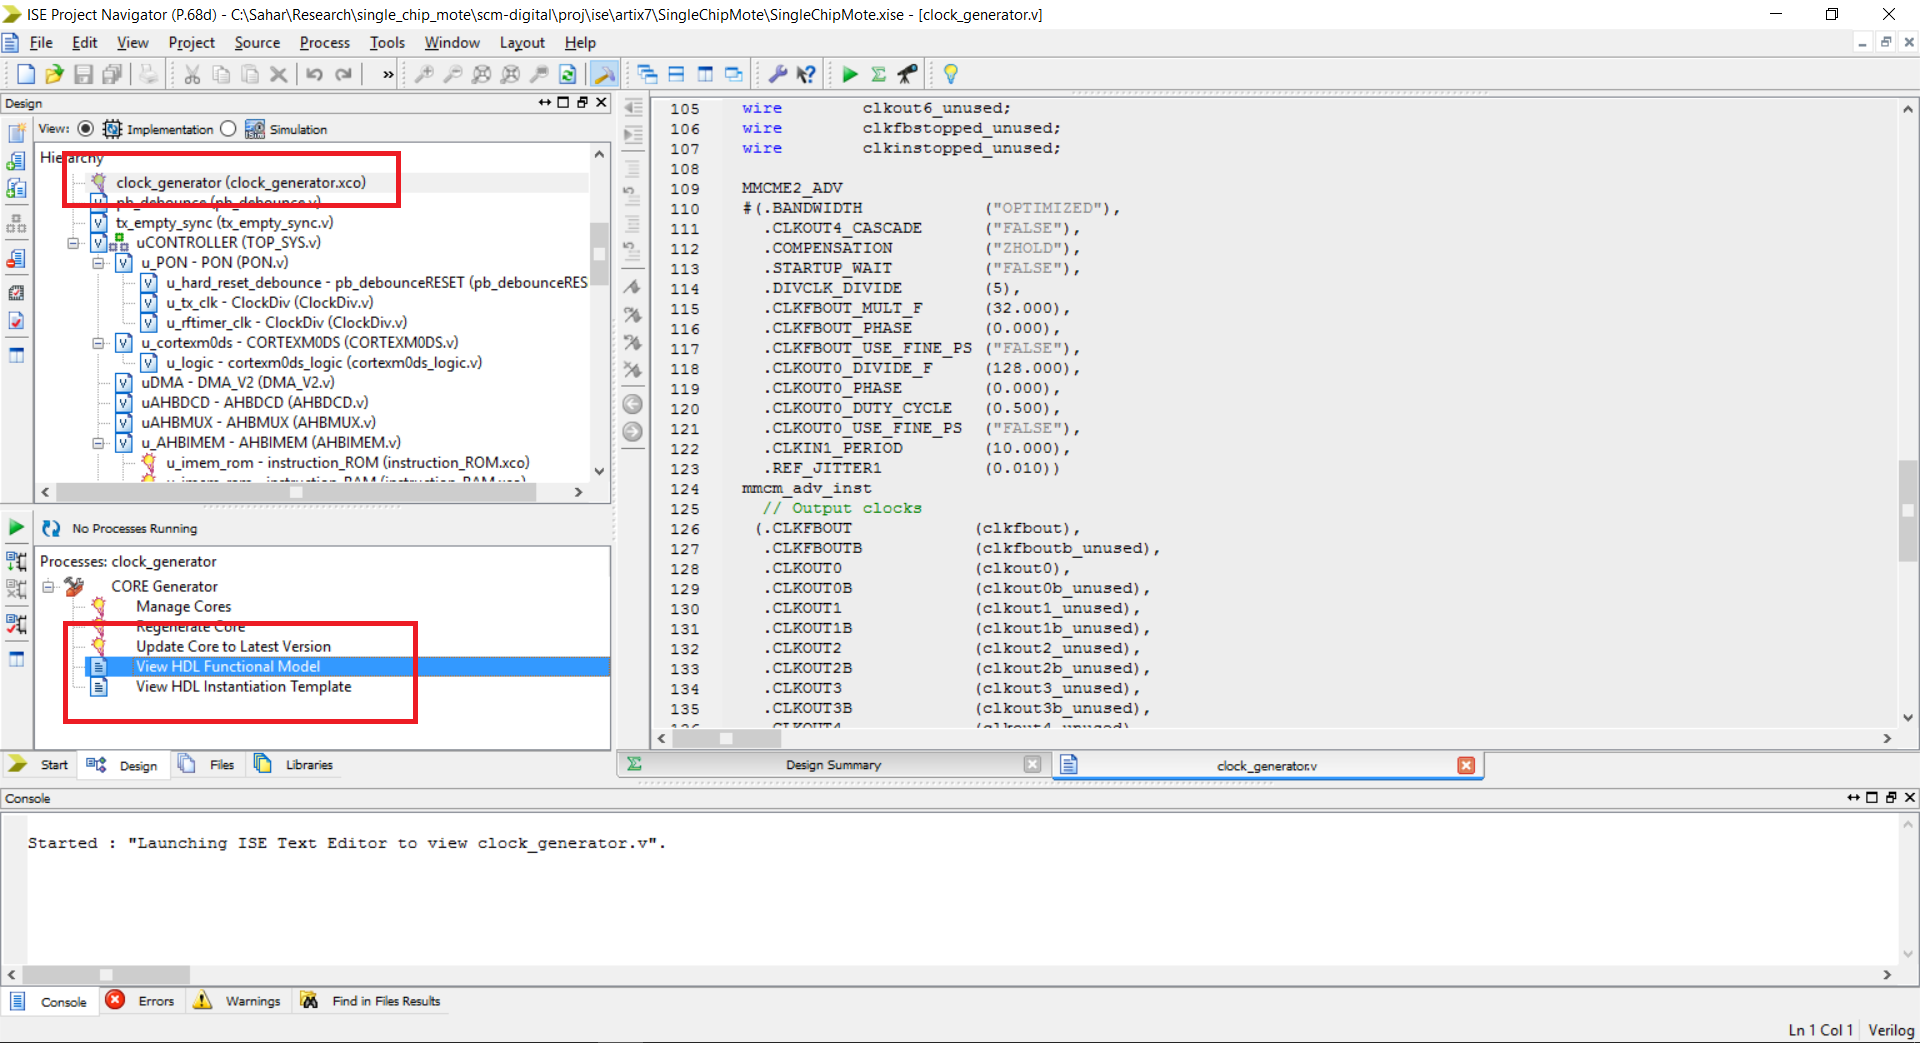
\includegraphics[width=1\linewidth]{clock-coregen}
\caption{View HDL Functional Model for a generated core}
\label{fig:clock-coregen}
\end{figure}
\begin{figure}
	\centering
	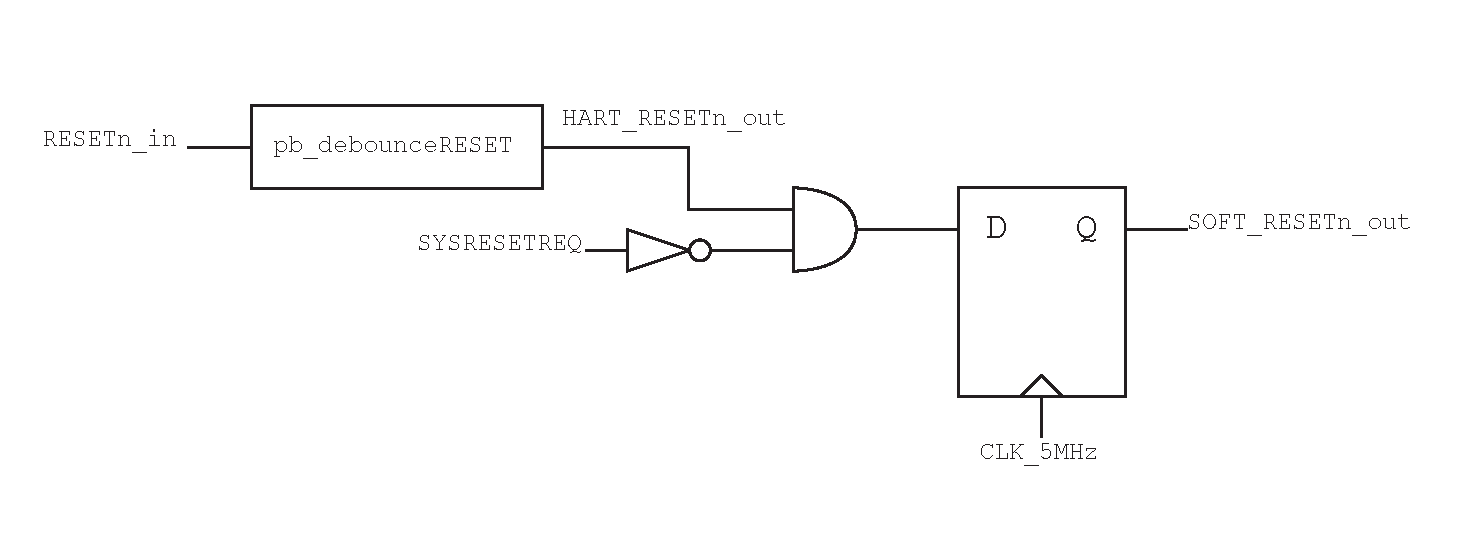
\includegraphics[width=1\linewidth]{resets}
	\caption{Reset handling in the \texttt{PON} module}
	\label{fig:resets}
\end{figure}

\section{pb\_debounceRESET}
\subsection{Description}
This module is used to debounce the output signal from a button on the FPGA board used as the reset input to the Single Chip Mote digital system. This module is a slightly modified version of the \texttt{pb\_debouce} module provided in the ARM Cortex-M0 DesignStart kit. Bigazzi modified this code such that the output is active-low instead of active-high.

\subsection{Input/Output Ports}
\begin{description}
	\item[\texttt{clk}] The input clock used to sample and synchronize the input signal.
	\item[\texttt{resetn}] Active-low reset input. This is not the reset signal that is being debounced. Instead, this is the reset signal used to reset the \texttt{pb\_debounceRESET} module itself. This is a remnant of the original \texttt{pb\_debounce} module and is not used in \texttt{pb\_debounceRESET} when instantiated inside the \texttt{PON} module. Therefore this signal is assigned to its inactive value, 1.
	\item[\texttt{pb\_in}] Input signal to be sampled and debouced. This is where the input reset signal is attached.
	\item[\texttt{pb\_out}] Stabilized output signal. This is a remnant of the original \texttt{pb\_debounce} module and is not used in \texttt{pb\_debounceRESET} when instantiated in the \texttt{PON} module. Therefore this output is ignored.
	\item[\texttt{pb\_tick}] Output pulse when the input has changed and is stable. When the input signal changes and the debouncer considers it stable, this active-high output changes to low for 1 cycle. This is used as the reset signal in the \texttt{PON} module.
\end{description}

\subsection{Design Details}
This module samples the \texttt{pb\_in} input using \texttt{clk}. When the input changes from 0 to 1, a counter begins counting down from \texttt{\{21\{1\'{}b1\}\}} to 0. If the signal remains stable by the time the counter reaches 0, the \texttt{pb\_out} output changes from 0 to 1. At the same time, the \texttt{pb\_tick} output, with a default value of 1, changes to 0 for a single cycle. When the input goes back to 0, the output follows. If the signal changes to 0 before the counter reaches 0, the counter is reset and the module waits for \texttt{pb\_in} to change again.

The button used for the reset signal on the Nexys 3 board is an active-high button. The output is low when the button is not pressed, and the output is high when the button is pressed. In contrast, the button used for the reset signal on the Nexys 4 DDR board is an active-low button, where the output is high when not pressed, and low when pressed. The same \texttt{pb\_debounceRESET} module is used for both, because the \texttt{pb\_tick} output is used for the reset output instead of the \texttt{pb\_out} output, and thus the behavior when a button is pressed is almost the same. The \texttt{pb\_tick} output sends an active-low single-cycle pulse when the input changes from low to high and is stable. In the case of the Nexys 3 this happens when the button is pressed and held. In the case of the Nexys 4 DDR this happens when a pressed button is released. It may be worthwhile in the future to modify the behavior of \texttt{pb\_debounceRESET} to work for both types of buttons using the \texttt{pb\_out} output instead. % the use of may here is justified

\section{ClockDiv}
\subsection{Description}
This module was originally designed by Bigazzi to divide the 100MHz input clock down to 5MHz. This module has since been parameterized to divide a clock down by any amount and is currently used to divide the 100MHz clock to 2MHz and 500kHz.

\subsection{Input/Output Ports and Parameters}
\begin{description}
	\item[\texttt{CLK\_IN}] Input clock to be divided.
	\item[\texttt{RESETn}] Input reset.
	\item[\texttt{CLK\_OUT}] Divided output clock.
	\item[\texttt{MAX\_COUNT}] Parameter describing the number of cycles to count before inverting the output clock signal.
\end{description}

\subsection{Design Details}
This clock divider is implemented with a counter that increments from 0 to \texttt{MAX\_COU\-N\-T-1} and then wraps around. Every time the counter reaches \texttt{MAX\_COUNT-1} the \texttt{CLK\_OUT} output inverts. The clock period of the output is:
$$ T_{out} = 2 \times MAX\_COUNT \times T_{in} $$
This method of clock division is not recommended on FPGAs; however, this method is the only way to generate clocks less than 2.5MHz given that there are no FPGA primitives able to divide a 100MHz clock below 2.5MHz.

\section{AHBDCD} \label{ahbdcd}
\subsection{Description}
This module, adapted from the example provided in the ARM Cortex-M0 DesignStart kit, is used to determine which AHB slave is being accessed during an AHB transfer. It decodes \texttt{HADDR[31:24]} to generate a \texttt{HSEL} signal for each slave, as well as the \texttt{MUL\_SEL[3:0]} signal sent to the \texttt{AHBMUX} module. This module supports up to 15 AHB slaves.

\subsection{Input/Output Ports}
\begin{description}
	\item[\texttt{HADDR[31:24]}] Address input. Only the 8 upper bits are necessary and the other bits are omitted.
	\item[\texttt{HSEL\_S0}] Slave select output for the first AHB slave. In the Single Chip Mote digital system this is the \texttt{AHBIMEM} module. The \texttt{AHBIMEM} module is connected to the AHB using two AHB interfaces, with one for fetching instructions and another for bootloading (chapter \ref{bootloading}). \texttt{HSEL\_S0} is for fetching instructions.
	\item[\texttt{HSEL\_S1}] Slave select output for the second AHB slave. In the Single Chip Mote digital system this is the AHBsub bus, via the \texttt{AHBLiteArbiter\_V2} module.
	\item[\texttt{HSEL\_S2}] Slave select output for the third AHB slave. In the Single Chip Mote digital system this is the \texttt{DMA\_V2} module.
	\item[\texttt{HSEL\_S3}] Slave select output for the fourth AHB slave. In the Single Chip Mote digital system this is the APB, via the \texttt{AHB2APB} module.
	\item[\texttt{HSEL\_S4}] Slave select output for the fifth AHB slave. In the Single Chip Mote digital system this is the \texttt{AHBIMEM} module. The \texttt{AHBIMEM} module is connected to the AHB using two AHB interfaces, with one for fetching instructions and another for bootloading (chapter \ref{bootloading}). \texttt{HSEL\_S4} is for bootloading.
	\item[\texttt{HSEL\_S5}] Slave select output for the sixth AHB slave. In the Single Chip Mote digital system this is the APB, via the \texttt{RFTIMER} module.
	\item[\texttt{HSEL\_NOMAP}] Slave select output indicating that the current address does not map to any AHB slaves. This output is omitted in the Single Chip Mote digital system.
	\item[\texttt{MUL\_SEL[3:0]}] Output to the \texttt{AHBMUX} module indicating which slave is selected. This is used to route the correct set of slave signals to the AHB master.
\end{description}

\subsection{Design Details}
This module only contains combinational logic to set the \texttt{HSEL} and \texttt{MUL\_SEL} outputs using the 8 upper bits of \texttt{HADDR}. This is done using a casex statement with the prefixes defined in \texttt{REGISTERS.vh}. A casex statement is used in order to facilitate the use one single prefix for all APB slaves, by having the 4 upper bits match \texttt{4\'{}b0101} and the 4 lower bits match \texttt{4\'{}bxxxx}. As long as the 4 upper bits of all APB slave prefixes begin with \texttt{4\'{}b0101}, then the \texttt{HSEL} signal for the APB bridge (\texttt{AHB2APB}) is correct.

Inside the casex statement, the 16-bit \texttt{dec} bus is assigned along with \texttt{MUX\_SEL}. If the case is for the nth slave (where n=0 for the first slave, n=1 for the second), then \texttt{dec[n]} must be assigned to 1. All other bits in \texttt{dec} must be assigned 0. \texttt{MUX\_SEL} must also be assigned to the binary value of n.

\subsection{Adding Another AHB Slave} \label{ahbdcd-new-slave}
Adding a new AHB slave in this module requires the following steps:

\begin{enumerate}
	\item Define an address prefix for the slave in \texttt{REGISTERS.vh}.
	\item Add another \texttt{HSEL} output.
	\item Add another case to the casex statement using the new address prefix. Make sure to set the \texttt{dec} and \texttt{MUX\_SEL} signals correctly as described above.
	\item Assign the new \texttt{HSEL} output to the corresponding bit in \texttt{dec}.
	\item Connect the new \texttt{HSEL} output to the new slave/peripheral in the top module, \texttt{uCONTROLLER}.
\end{enumerate}

\section{AHBMUX} \label{ahbmux}
\subsection{Description}
This module, adapted from the example provided in the ARM Cortex-M0 DesignStart kit, is used to select the correct set of AHB slave signals (\texttt{HRDATA} and \texttt{HREADYOUT}) from the APB slave being accessed during the current transfer. The slave signals are chosen based on the \texttt{MUX\_SEL} signal provided by \texttt{AHBDCD}. This module supports up to 15 slaves.

\subsection{Input/Output Ports}
\begin{description}
	\item[\texttt{HCLK}] Input clock.
	\item[\texttt{HRESETn}] Input reset.
	\item[\texttt{MUX\_SEL[3:0]}] Input from \texttt{AHBDCD} indicating which AHB slave is selected for the current transfer.
	\item[\texttt{HRDATA\_S0[31:0]}] Read data input from the first AHB slave. In the Single Chip Mote digital system this is the \texttt{AHBIMEM} module. The \texttt{AHBIMEM} module is connected to the AHB using two AHB interfaces, with one for fetching instructions and another for bootloading (chapter \ref{bootloading}). \texttt{HRDATA\_S0} is for fetching instructions.
	\item[\texttt{HRDATA\_S1[31:0]}] Read data input from the second AHB slave. In the Single Chip Mote digital system this is the AHBsub bus, via the \texttt{AHBLiteArbiter\_V2} module.
	\item[\texttt{HRDATA\_S2[31:0]}] Read data input from the third AHB slave. In the Single Chip Mote digital system this is the \texttt{DMA\_V2} module.
	\item[\texttt{HRDATA\_S3[31:0]}] Read data input from the fourth AHB slave. In the Single Chip Mote digital system this is the APB, via the \texttt{AHB2APB} module.
	\item[\texttt{HRDATA\_S4[31:0]}] Read data input from the fifth AHB slave. In the Single Chip Mote digital system this is the \texttt{AHBIMEM} module. The \texttt{AHBIMEM} module is connected to the AHB using two AHB interfaces, with one for fetching instructions and another for bootloading (chapter \ref{bootloading}). \texttt{HRDATA\_S4} is for bootloading.
	\item[\texttt{HRDATA\_S5[31:0]}] Read data input from the sixth AHB slave. In the Single Chip Mote digital system this is the \texttt{RFTIMER} module.
	\item[\texttt{HRDATA\_NOMAP[31:0]}] Read data input to be used when the current address does not map to any AHB slaves.
	\item[\texttt{HREADYOUT\_S0}] Transfer finished input from the first AHB slave. In the Single Chip Mote digital system this is the \texttt{AHBIMEM} module. The \texttt{AHBIMEM} module is connected to the AHB using two AHB interfaces, with one for fetching instructions and another for bootloading (chapter \ref{bootloading}). \texttt{HREADYOUT\_S0} is for fetching instructions.
	\item[\texttt{HREADYOUT\_S1}] Transfer finished input from the second AHB slave. In the Single Chip Mote digital system this is the AHBsub bus, via the \texttt{AHBLiteArbiter\_V2} module.
	\item[\texttt{HREADYOUT\_S2}] Transfer finished input from the third AHB slave. In the Single Chip Mote digital system this is the \texttt{DMA\_V2} module.
	\item[\texttt{HREADYOUT\_S3}] Transfer finished input from the fourth AHB slave. In the Single Chip Mote digital system this is the APB, via the \texttt{AHB2APB} module.
	\item[\texttt{HREADYOUT\_S4}] Transfer finished input from the fifth AHB slave. In the Single Chip Mote digital system this is the \texttt{AHBIMEM} module. The \texttt{AHBIMEM} module is connected to the AHB using two AHB interfaces, with one for fetching instructions and another for bootloading (chapter \ref{bootloading}). \texttt{HREADYOUT\_S4} is for bootloading.
	\item[\texttt{HREADYOUT\_S5}] Transfer finished input from the sixth AHB slave. In the Single Chip Mote digital system this is the \texttt{RFTIMER} module.
	\item[\texttt{HREADYOUT\_NOMAP}] Transfer finish input to be used when the current address does not map to any AHB slaves. This input must always be assigned to 1 to avoid indefinitely stalling the Cortex-M0 if it tries to access an unmapped address.
	\item[\texttt{HREADY}] Multiplexed transfer finish output to the AHB master.
	\item[\texttt{HRDATA[31:0]}] Multiplexed read data output to the AHB master.
\end{description}

\subsection{Design Details}
The address, \texttt{HADDR}, is valid during an address phase of a transfer, and therefore that the \texttt{MUX\_SEL} is also only valid during the address phase. The \texttt{MUX\_SEL} signal must be latched before moving on to the data phase. This is done by storing \texttt{MUX\_SEL} into a register, \texttt{APHASE\_MUX\_SEL}, whenever \texttt{HREADY} is 1. \texttt{APHASE\_MUX\_SEL} is then used in a case statement to assign the correct slave signals to \texttt{HRDATA} and \texttt{HREADY}.

\subsection{Adding Another AHB Slave}
Adding a new AHB slave in this module requires the following steps:

\begin{enumerate}
	\item Add this slave to \texttt{AHBDCD}. See section \ref{ahbdcd-new-slave} for more details.
	\item Add another \texttt{HRDATA} and \texttt{HREADYOUT} input.
	\item Add another case to the case statement using the new value of \texttt{MUX\_SEL} corresponding to the new slave. Assign \texttt{HRDATA} and \texttt{HREADY}.
	\item Connect the new \texttt{HRDATA} and \texttt{HREADYOUT} inputs to the new slave/peripheral in the top module, \texttt{uCONTROLLER}.
\end{enumerate}

\section{AHBLiteArbiter\_V2}
\subsection{Description}
This module is an arbiter designed to allow for two masters (referred to as M0 and M1) to share a single AHB-Lite bus. This module is necessary in order to allow the Cortex-M0 and the DMA to both access the data memory and the radio controller via the AHBsub bus. Master M0 is the Cortex-M0, via the main AHB bus. Master M1 is the DMA. In this module, the slave refers to the AHBsub bus. The intended behavior of this arbiter is as follows:

\begin{itemize}
	\item M0 does not experience any latency for any AHB transfers when M1 is not attempting to transfer at the same time. This means that, while the DMA is idle, the Cortex-M0 has to access both the data memory and radio controller as if it were on the main AHBbus, with no extra latency.
	\item M1 may experience at least 1 cycle of additional latency when accessing the bus, even if master M0 is idle. This is a consequence of the previous rule. % the use of may here is justified
	\item When both M0 and M1 initiate a transfer at the same time, after a period of no transfers, M0 has priority. Initiating a transfer means the master asserts \texttt{HTRANS[1]} and \texttt{HSEL}; this also indicates the address phase of the transfer.
	\item When both M0 and M1 initiate a transfer at the same time, during a series of back-to-back transfers, the master that was not granted the last transfer is granted the next transfer.
\end{itemize}

Given that the AHBsub bus is primarily used by the Cortex-M0 to access data memory, it is important that the Cortex-M0 experience no latency when accessing the data memory under normal conditions. In contrast, the DMA only accesses the AHBsub bus when the Single Chip Mote is sending or receiving a radio packet, and the relatively slow data rate does not require that the DMA have high throughput or low latency. Therefore, it is acceptable to have additional latency for M1 and give priority during an initial collision to M0.

\subsection{Input/Output Ports}
\begin{description}
	\item[\texttt{HCLK}] Input clock.
	\item[\texttt{HRESETn}] Input reset.
	
	\item[\texttt{HSEL\_M0}] Slave select input from master M0.
	\item[\texttt{HADDR\_M0[31:0]}] Address input from master M0.
	\item[\texttt{HTRANS\_M0[1]}] Transfer type input from master M0.
	\item[\texttt{HSIZE\_M0[1:0]}] Transfer size input from master M0.
	\item[\texttt{HWRITE\_M0}] Write select input from master M0.
	\item[\texttt{HWDATA\_M0[31:0]}] Write data input from master M0.
	\item[\texttt{HRDATA\_M0[31:0]}] Read data output to master M0.
	\item[\texttt{HREADY\_M0}] Transfer finished output to master M0.

	\item[\texttt{HSEL\_M1}] Slave select input from master M1.
	\item[\texttt{HADDR\_M1[31:0]}] Address input from master M1.
	\item[\texttt{HTRANS\_M1[1]}] Transfer type input from master M1.
	\item[\texttt{HSIZE\_M1[1:0]}] Transfer size input from master M1.
	\item[\texttt{HWRITE\_M1}] Write select input from master M1.
	\item[\texttt{HWDATA\_M1[31:0]}] Write data input from master M1.
	\item[\texttt{HRDATA\_M1[31:0]}] Read data output to master M1.
	\item[\texttt{HREADY\_M1}] Transfer finished output to master M1.
	
	\item[\texttt{HADDR\_S[31:0]}] Address output to slave.
	\item[\texttt{HTRANS\_S[1]}] Transfer type output to slave.
	\item[\texttt{HSIZE\_S[1:0]}] Transfer size output to slave.
	\item[\texttt{HWRITE\_S}] Write select output to slave.
	\item[\texttt{HWDATA\_S[31:0]}] Write data output to slave.
	\item[\texttt{HRDATA\_S[31:0]}] Read data input from slave.
	\item[\texttt{HREADYOUT\_S}] Transfer finished input from slave.
	
	\item[\texttt{error}] Indicates that the arbiter reached an invalid state at some point. This signal is included for debugging purposes but is typically ignored. Currently, synthesis tools remove this signal during optimization.
\end{description}

\subsection{Design Details}
ARM provides in their Cortex-M System Design Kit \cite{cmsdk} a bus matrix designed to allow for multiple masters to control a single AHB bus or even a single AHB slave. This module is both flexible in its use and allows for customization, and also benefits from being tested and proven to work. Unfortunately, the System Design Kit is not part of the DesignStart kit and must be purchased separately. There were multiple attempts prior to this work by visiting scholars Francesco Bigazzi and Lorenz Schmid (both working independently) to create a simplified but analogous arbiter design, all of which failed to function without error on real-time FPGA tests. Arbitration errors caused unpredictable behavior when both masters attempted to access peripherals on the AHBsub bus at the same time.

\subsubsection{Design Issues}
The main cause of difficulty in the design of this arbiter is the inability to completely describe its function in the form of a finite state machine or a series of basic rules/steps. This is attributed to the following complications:

\begin{itemize}
	\item AHB transfers happen in two phases, the address and data phase. The arbiter must have a way to keep track of the phases for each master.
	\item AHB transfers can be pipelined, and each master could be in both the address and data phase at the same time.
	\item The AHB protocol expects that the slave latches address phase signals when necessary because of pipelined transfers. Given that there are two masters, this means that the each master must be tracked to ensure that address phase signals are latched properly when one master is stalled.
\end{itemize}

These complications imply that the arbiter must keep track of the following state:

\begin{itemize}
	\item Which master's address phase signals are routed to the slave.
	\item Which master's dataphase signals are routed to the slave.
	\item Which master is connected to the slave's dataphase signals. This concerns the \texttt{HREADYOUT\_S} signal in particular, as the stalled master must \textit{not} see the \texttt{HREADYOUT\_S} signal when the other master is using the bus.
	\item If either of the masters have address phase signals latched from when the other master was using the bus.
\end{itemize}

And the arbiter must make the following decisions depending on the state:

\begin{itemize}
	\item Which master's address phase signals to route to the slave during the next cycle. This includes address phase signals that were latched from a stalled master. This is where the arbitration takes place; the result depends on which master is currently using the bus.
	\item Which master's data phase signals to route to the slave during the next cycle. This depends on whether or not the transfer is complete (\texttt{HREADYOUT\_S} is asserted), and which address phase signals are currently routed to the slave.
	\item Whether or not any address phase signals need to be latched because one master must be stalled. Address phase signals only need to be latched when the master is not waiting for its own data phase to finish. When the master is waiting for a data phase to complete, it is sufficient to keep \texttt{HREADY} low. This stalls the master causing it to continue to hold its address phase signals. However, if the master is not waiting (from its point of view it is initiating its first transfer after being idle), the master assumes the slave latches the address phase signals and only holds the valid signals for 1 cycle. This behavior is a consequence of pipelined transfers in the AHB protocol.
\end{itemize}

The amount of state that must be tracked for both masters and the slave makes it difficult to create a concise description of the arbiter's behavior. It was eventually determined that the best way to design this module was to enumerate every possible state and determine the actions and next state in a large table. From there, the address phase and data phase signals could be routed properly and the combinational logic to describe the table could be written in Verilog. While this solution is far from the best possible design practice, the current \texttt{AHBLiteArbiter\_V2} implementation continuously proves to work properly when tested in real-time on an FPGA.

\subsubsection{State Variables and Inputs}
The state variables used to route signals and determine the next state in this module are:

\begin{description}
	\item[\texttt{current\_address\_phase[1:0]}] This state describes which set of address phase signals are currently routed to the slave. Possible values are \texttt{APHASE\_PASS\_M0}, \texttt{APHASE\_LATCH\_M0}, and \texttt{APHASE\_LATCH\_M1}.
	\item[\texttt{current\_data\_phase[1:0]}] This state describes which set of data phase signals are currently routed to the slave and back. Possible values are \texttt{DPHASE\_NONE}, \texttt{DPHASE\_M0}, and \texttt{DPHASE\_M1}.
	\item[\texttt{inputs\_latched\_M0}] This state indicates whether or not there are currently any latched address signals from M0. This can happen when M0 must be stalled while the bus is in use. This state is needed when determining the next address phase.
	\item[\texttt{inputs\_latched\_M1}] This state indicates whether or not there are currently any latched address signals from M1. This can happen when M1 must be stalled while the bus is in use. This also happens when M1 uses the bus after an idle period since M0 continues to have priority when idle, and its address phase signals are always connected to the slave when idle. This state is needed when determining the next address phase.
\end{description}

In addition to the state variables, the following inputs are needed to determine the next state in this module:

\begin{description}
	\item[\texttt{req\_M0}] This signal is the bitwise AND of the \texttt{HSEL\_M0} and \texttt{HTRANS\_M0[1]} inputs, used to indicate that M0 is requesting use of the bus. This combination of inputs is needed when determining the next address phase.
	\item[\texttt{req\_M1}] This signal is the bitwise AND of the \texttt{HSEL\_M1} and \texttt{HTRANS\_M1[1]} inputs, used to indicate that M1 is requesting use of the bus. This combination of inputs is needed when determining the next address phase.
\end{description}

\subsubsection{Combinational Logic Based on State Variables and Inputs}
The \texttt{current\_address\_phase} state is used to route the address phase signals from one of the masters to the slave, and the \texttt{current\_data\_phase} state is used to route the dataphase signals between one master and the slave. 

\texttt{APHASE\_PASS\_M0} means that address phase signals are passed directly from M0 to the slave, with no registers in between. \texttt{APHASE\_LATCH\_M0} means that address phase signals latched from M0 during a previous cycle are routed to the slave. \texttt{APHASE\_LATCH\_M1} means that address phase signals latched from M1 during a previous cycle are routed to the slave. The default value is \texttt{APHASE\_PASS\_M0}.

\texttt{DPHASE\_NONE} means that all data phase signals are 0 because neither master is waiting for a slave. \texttt{DPHASE\_M0} means that \texttt{HWDATA\_M0} is routed to the slave, \texttt{HREADYOUT\_S} is routed to \texttt{HREADY\_M0}, and \texttt{HREADY\_M1} is 0. \texttt{DPHASE\_M1} means that \texttt{HWDATA\_M1} is routed to the slave, \texttt{HREADYOUT\_S} is routed to \texttt{HREADY\_M1}. and \texttt{HREADY\_M0} is 0.

In addition to choosing the next state, new address phase signals may need to be latched or cleared. This is indicated by the \texttt{latch\_M0}, \texttt{latch\_M1}, \texttt{clr\_M0}, and \texttt{clr\_M1} signals assigned within the next state logic. % the use of may here is justified

\subsubsection{State Transition and Action Table}
Appendix \ref{appendix:arb-fsm} contains the table listing the inputs, state variables, next state, and actions to be taken, for every combination of state and input. This table was used to implement the next state combinational logic in \texttt{AHBLiteArbiter\_V2}. Note that some states are labeled as ``invalid state''; these states should be impossible to reach. However, the code is designed such that if one of those states were detected, the \texttt{error} output is set to 1 and stays that way until the system is reset. % the use of should is justified here

\section{AHBDCDsub}
\subsection{Description}
This module is the same as the \texttt{AHBDCD} module described in section \ref{ahbdcd}. The main difference is that this module is designed to be used for the AHBsub bus and has two slaves: the \texttt{AHBDMEM} module and the \texttt{RFcontroller} module. Also, the width of the \texttt{MUX\_SEL} signal is reduced such that this module now only supports three slaves.

\subsection{Input/Output Ports}
\begin{description}
	\item[\texttt{HADDR[31:24]}] Address input. Only the 8 upper bits are necessary and the other bits are omitted.
	\item[\texttt{HSEL\_S0}] Slave select output for the first AHB slave. In the Single Chip Mote digital system this is the \texttt{AHBDMEM} module.
	\item[\texttt{HSEL\_S1}] Slave select output for the second AHB slave. In the Single Chip Mote digital system this is the \texttt{RFcontroller} module.
	\item[\texttt{HSEL\_NOMAP}] Slave select output indicating that the current address does not map to any AHB slaves. This output is omitted in the Single Chip Mote digital system.
	\item[\texttt{MUL\_SEL[1:0]}] Output to the \texttt{AHBMUX} module indicating which slave is selected. This is used to route the correct set of slave signals to the AHB master.
\end{description}

\subsection{Design Details}
See section \ref{ahbdcd}.

\subsection{Adding Another AHB Slave}
See section \ref{ahbdcd}.

\section{AHBMUXsub}
\subsection{Description}
This module is the same as the \texttt{AHBMUX} module described in section \ref{ahbmux}. The main difference is that this module is designed to be used for the AHBsub bus and has two slaves: the \texttt{AHBDMEM} module and the \texttt{RFcontroller} module. Also, the width of the \texttt{MUX\_SEL} signal is reduced such that this module now only supports three slaves.

\subsection{Input/Output Ports}
\begin{description}
	\item[\texttt{HCLK}] Input clock.
	\item[\texttt{HRESETn}] Input reset.
	\item[\texttt{MUX\_SEL[3:0]}] Input from \texttt{AHBDCD} indicating which AHB slave is selected for the current transfer.
	\item[\texttt{HRDATA\_S0[31:0]}] Read data input from the first AHB slave. In the Single Chip Mote digital system this is the \texttt{AHBDMEM} module.
	\item[\texttt{HRDATA\_S1[31:0]}] Read data input from the second AHB slave. In the Single Chip Mote digital system this is the \texttt{RFcontroller} module.
	\item[\texttt{HRDATA\_NOMAP[31:0]}] Read data input to be used when the current address does not map to any AHB slaves.
	\item[\texttt{HREADYOUT\_S0}] Transfer finished input from the first AHB slave. In the Single Chip Mote digital system this is the \texttt{AHBDMEM} module.
	\item[\texttt{HREADYOUT\_S1}] Transfer finished input from the second AHB slave. In the Single Chip Mote digital system this is the \texttt{RFcontroller} module.
	\item[\texttt{HREADYOUT\_NOMAP}] Transfer finish input to be used when the current address does not map to any AHB slaves. This input must always be assigned to 1 to avoid indefinitely stalling the Cortex-M0 if it tries to access an unmapped address.
	\item[\texttt{HREADY}] Multiplexed transfer finish output to the AHB master.
	\item[\texttt{HRDATA[31:0]}] Multiplexed read data output to the AHB master.
\end{description}

\subsection{Design Details}
See section \ref{ahbmux}.

\subsection{Adding Another AHB Slave}
See section \ref{ahbmux}.

\section{AHBIMEM} \label{AHBIMEM}
\subsection{Description}
This module provides access to the instruction memory for the Cortex-M0. The instruction memory is composed of a 16kB ROM and a 64kB SRAM (referred to from now on as the instruction RAM). Only one of the two memories are in use at any particular time. Instructions are fetched from the ROM when the Single Chip Mote digital system initially turns on, or after a hard reset. The code in the ROM is designed to load the main software code into the RAM, and then initiate a soft reset. After the soft reset, instructions are fetched from the RAM. The main software code is written into the RAM directly through an external 3 Wire Bus interface, or via the AHB bus from the Cortex-M0. The Cortex-M0 has the option to listen for instructions via UART, over the radio, or even through an optical interface (this has not been designed yet). For more information on bootloading, see chapter \ref{bootloading}.

This module has two AHB slave interfaces. The first slave interface is used to read from the instruction memory. The \texttt{HWRITE} signal is ignored, as instruction memory is considered read-only, even when the SRAM is in use. All instruction fetches are assumed to be the size of a word (32 bits) and word-aligned, and therefore the \texttt{HSIZE} signal from the AHB is omitted. The second slave interface is used to load data into the instruction RAM. This interface has one special address allocated for a configuration register. All other addresses correspond to an address in the instruction RAM. AHB writes overwrite data in either the configuration register or the instruction RAM. AHB reads return the contents of a special status register, regardless of the address used. All writes are assumed to be the size of a word (32 bits) and word-aligned, and therefore the \texttt{HSIZE} signal from the AHB is omitted.

\subsection{Input/Output Ports and Parameters}
\begin{description}
	\item[\texttt{RESETn}] Hard reset input. This reset is triggered externally from the FPGA board.
	\item[\texttt{HRESETn}] Soft reset input. This reset is triggered either externally from the FPGA board or internally via a reset request from the Cortex-M0.
	\item[\texttt{HSEL\_IMEM}] Slave select input for the instruction memory AHB interface.
	\item[\texttt{HSEL\_BOOTLOAD}] Slave select input for the bootloading AHB interface.
	\item[\texttt{HREADY}] Transfer finished input. This input indicates that the previous transfer on the bus has finished and that address phase signals must be latched.
	\item[\texttt{HADDR[31:0]}] Address input.
	\item[\texttt{HTRANS[1]}] Transfer type input.
	\item[\texttt{HWRITE}] Write select input.
	\item[\texttt{HWDATA[31:0]}] Write data input.
	\item[\texttt{HREADYOUT\_IMEM}] Transfer finished output from the instruction memory AHB interface.
	\item[\texttt{HRDATA\_IMEM[31:0]}] Read data output from the instruction memory AHB interface.\item[\texttt{HREADYOUT\_BOOTLOAD}] Transfer finished output from the bootloading AHB interface.
	\item[\texttt{HRDATA\_BOOTLOAD[31:0]}] Read data output from the bootloading AHB interface.
	\item[\texttt{clk\_3wb}] Clock input for the 3 Wire Bus.
	\item[\texttt{data\_3wb}] Data input for the 3 Wire Bus.
	\item[\texttt{latch\_3wb}] Latch input for the 3 Wire Bus.
	\item[\texttt{clk\_3wb\_en}] Clock enable output to disable \texttt{clk\_3wb} when not in use.
	\item[\texttt{ROM\_ADDR\_WIDTH}] Parameter describing the size of the instruction ROM. The number of address bits needed for the word-addressable instruction ROM is equal to this parameter, and the depth of the instruction ROM is $2^{ROM\_ADDR\_WIDTH}$. Note that the addresses in \texttt{HADDR} are byte, not word, addresses.
	\item[\texttt{RAM\_ADDR\_WIDTH}] Parameter describing the size of the instruction RAM. The number of address bits needed for the word-addressable instruction RAM is equal to this parameter, and the depth of the instruction RAM is $2^{RAM\_ADDR\_WIDTH}$. Note that the addresses in \texttt{HADDR} are byte, not word, addresses.
\end{description}

\subsection{Design Details}
This module uses the \texttt{imem\_mode} register to determine the source of instruction data, and connects that source to the AHB interface for fetching instructions. Instruction data can come from either the ROM or the RAM, and therefore, the two possible states for the \texttt{imem\_mode} register are \texttt{IMEM\_MODE\_ROM} and \texttt{IMEM\_MODE\_RAM}. The \texttt{imem\_mode} register is only updated on a hard or soft reset, to ensure that the source of instruction data does not change while the Single Chip Mote digital system is running. On a hard reset, \texttt{imem\_mode} is set by default to \texttt{IMEM\_MODE\_ROM}. On a soft reset, \texttt{imem\_mode} is set to the value stored in the \texttt{next\_imem\_mode} register. This register is set by the Cortex-M0 via the bootloading AHB interface to be either \texttt{IMEM\_MODE\_ROM} or \texttt{IMEM\_MODE\_RAM}. Figure \ref{table:boot-imem-mode} contains the encoded values for \texttt{IMEM\_MODE\_RAM} and \texttt{IMEM\_MODE\_ROM}.

\begin{figure}
	\centering
	\begin{tabular}{|c|c|}
		\hline
		\texttt{imem\_mode} & Encoding \\
		\hline
		\texttt{IMEM\_MODE\_ROM} & \texttt{1'b0} \\
		\texttt{IMEM\_MODE\_RAM} & \texttt{1'b1} \\
		\hline
	\end{tabular}
	\caption{Encodings for the two \texttt{imem\_mode} states}
	\label{table:boot-imem-mode}
\end{figure}


This module uses the \texttt{boot\_mode} register to determine from which source the instruction RAM is written. The three possible states for this register are \texttt{BOOT\_MODE\-\_NONE}, \texttt{BOOT\_MODE\_3WB}, and \texttt{BOOT\_MODE\_AHB}. \texttt{BOOT\_MODE\_NONE} means that the instruction RAM cannot be written. \texttt{BOOT\_MODE\_3WB} means that the instruction RAM is written externally via the 3 Wire Bus. \texttt{BOOT\_MODE\_AHB} means that the instruction RAM is written by the Cortex-M0 via the bootloading AHB interface. This state register is configured by the Cortex-M0 via the bootloading AHB interface. Figure \ref{table:boot-boot-mode} contains the encoded values for all three boot modes.

\begin{figure}
	\centering
	\begin{tabular}{|c|c|}
		\hline
		\texttt{boot\_mode} & Encoding \\
		\hline
		\texttt{BOOT\_MODE\_NONE} & \texttt{2'b00} \\
		\texttt{BOOT\_MODE\_3WB} & \texttt{2'b10} \\
		\texttt{BOOT\_MODE\_AHB} & \texttt{2'b11} \\
		\hline
	\end{tabular}
	\caption{Encodings for the three \texttt{boot\_mode} states}
	\label{table:boot-boot-mode}
\end{figure}

When the \texttt{boot\_mode} register is set to \texttt{BOOT\_MODE\_3WB}, the \texttt{AHBIMEM} module enables the 3 Wire Bus clock input (using \texttt{clk\_3wb\_en}), and waits for 64kB of data to be written into the instruction RAM. This is accomplished using a counter, doubling as the write address to the instruction RAM. This counter is initialized to 0 on a soft reset, and increments as each 32-bit word is written into the RAM. Once this counter has reached its maximum value, indicating that 64kB has been written to the RAM, the \texttt{boot\_3wb\_done} signal is asserted, and all other writes via the 3 Wire Bus are disabled. The 3 Wire Bus clock is also disabled. For more information on the 3 Wire Bus protocol, see section \ref{3wb}.

When the \texttt{boot\_mode} register is set to \texttt{BOOT\_MODE\_AHB}, the \texttt{AHBIMEM} module connects the write port of the instruction RAM to the bootloading AHB interface. This allows for the Cortex-M0 to write directly into the instruction RAM (although it cannot read what is in the instruction RAM). The two AHB interfaces correspond to two separate AHB slaves with their own address prefixes. The prefix for the instruction fetching interface is \texttt{0x00} and the prefix for the bootloading interface is \texttt{0x01}. Any writes to the RAM via the bootloading interface result in a write to the corresponding address in the RAM where the \texttt{0x01} prefix is replaced with \texttt{0x00}. For example, writing an instruction to address \texttt{0x0100CAD0} translates to address \texttt{0x0000CAD0} in the actual instruction memory. Since the instruction RAM is only 64kB, any writes to addresses beyond the first 64kB of instruction memory result in overwriting instruction data within the first 64kB.

The bootloading AHB interface also has a dedicated write-only configuration register used to change \texttt{next\_imem\_mode} and \texttt{boot\_mode}. Any AHB read transfer, regardless of the address, from the bootloading AHB interface result in reading the status register. This status register returns the values of \texttt{imem\_mode}, \texttt{next\_imem\_mode}, \texttt{boot\_mode}, and \texttt{boot\_3wb\_done}. See the next section for details on these registers.

\subsection{Register Interface}
\subsubsection{AHB Interface for Instruction Fetching}
This AHB interface has no memory-mapped registers. All reads return instruction data at the corresponding address in either the ROM or the RAM, and writes have no effect. Valid addresses are in the range of \texttt{0x00000000-0x0000FFFF} for a memory size of 64kB.

\subsubsection{AHB Interface for Bootloading}
This AHB interface is used to write to the instruction RAM, and has one read-only memory-mapped register and one write-only memory-mappped register. The first 64kB of addresses, \texttt{0x01000000-0x0100FFFF}, are allocated to the write-only instruction RAM. The address \texttt{0x01F00000} corresponds to the write-only \texttt{BOOTLOADER\-\_REG\-\_\_CFG} register. The fields of this register are \texttt{boot\_mode} and \texttt{next\_imem\_mode}. Reading from any register with the \texttt{0x01} prefix returns the \texttt{BOOTLOADER\_REG\_\_STAT\-US} register. The fields of this register contain \texttt{imem\_mode}, \texttt{next\_imem\_mode}, \texttt{boot\-\_mode}, and \texttt{boot\_3wb\_done}.

\subsubsection{Register Descriptions}
\ExecuteMetaData[chapters/registers.tex]{bootloader-registers}

\section{instruction\_ROM}
\subsection{Description}
This module is a 16kB read-only memory constructed out of FPGA primitives using CORE Generator. This ROM has a width of 32 bits and a depth of 4096, a read enable port, and a read latency of 1 cycle. This ROM is initialized with a COE file containing the compiled binary C code for the bootloading firmware. See chapter \ref{bootloading} for more information on bootloading.

\subsection{Input/Output Ports}
\begin{description}
	\item[\texttt{clka}] Input clock for the read port.
	\item[\texttt{ena}] Enable input for the read port.
	\item[\texttt{addra[11:0]}] Address input for the read port.
	\item[\texttt{douta[31:0]}] Data output for the read port. This data is valid 1 cycle after \texttt{ena} is asserted.
\end{description}

\subsection{Design Details}
The ROM was designed using the Block Memory Generator in CORE Generator. Any changes to the parameters of this module, such as the width or depth, requires opening the \texttt{instruction\_ROM.xco} file in CORE Generator, changing the parameters, and then regenerating the core. To open this design in CORE Generator, open Project Navigator and double-click the \texttt{instruction\_ROM} module in the Design Hierarchy panel.

\subsection{Initialization} \label{instruction-ROM}
Initializing the ROM requires a COE file containing data with the same width as the ROM, and a depth less than or equal to the depth of the ROM. In the case of the Single Chip Mote digital system, the COE file used to initialize the instruction ROM contains the compiled C binary code for the bootloading firmware. This firmware is first compiled into a binary (.bin) file using Keil. From there the Bin2coe tool (\ref{bin2coe}) is used to convert the binary file into a COE file. And finally, the \texttt{instruction\_ROM.xco} file must be opened in CORE Generator, wherein there is an option to specify a COE file to initialize the instruction ROM. Then the core must be generated again after entering the proper specifications. Any changes to the COE file require regeneration of the core.

\section{instruction\_RAM} \label{instruction-RAM}
\subsection{Description}
This module is a 64kB simple dual port SRAM constructed out of FPGA primitives using CORE Generator. This RAM has a width of 32 bits and a depth of 16384. The first port is for writing and the second port is for reading. The read port has a read enable input, with a read latency of 1 cycle. The write port contains separate write enable inputs for each byte 8-bit byte in the wordline (4 write enable inputs in total), and writes take effect after a single cycle.

\subsection{Input/Output Ports}
\begin{description}
	\item[\texttt{clka}] Input clock for the write port.
	\item[\texttt{ena}] Enable input for the write port. This must be asserted to write, even if \texttt{wea} is asserted.
	\item[\texttt{wea[3:0]}] Write enable input for each byte for the write port.
	\item[\texttt{addra[13:0]}] Address input for the write port.
	\item[\texttt{dina[31:0]}] Data input for the write port.
	\item[\texttt{clkb}] Input clock for the read port.
	\item[\texttt{enb}] Enable input for the read port.
	\item[\texttt{addrb[13:0]}] Address input for the read port.
	\item[\texttt{doutb[31:0]}] Data output for the read port. This data is valid 1 cycle after \texttt{ena} is asserted.
\end{description}

\subsection{Design Details}
The RAM was designed using the Block Memory Generator in CORE Generator. Any changes to the parameters of this module, such as the width or depth, requires opening the \texttt{instruction\_RAM.xco} file in CORE Generator, changing the parameters, and then regenerating the core. To open this design in CORE Generator, open Project Navigator and double-click the \texttt{instruction\_RAM} module in the Design Hierarchy panel.

\section{AHBDMEM}
\subsection{Description}
This module provides access to the data memory for the Cortex-M0. The data memory is composed of a 64kB SRAM with a width of 32 bits and a depth of 16384. This module supports byte, half-word, and word sized writes using the \texttt{HSIZE} input from the AHB. This module is based on the \texttt{AHB2MEM} module provided in the ARM Cortex-M0 DesignStart kit.

\subsection{Input/Output Ports and Parameters}
\begin{description}
	\item[\texttt{HCLK}] Input clock.
	\item[\texttt{HRESETn}] Input reset.
	\item[\texttt{HSEL}] Slave select input.
	\item[\texttt{HREADY}] Transfer finished input. This input indicates that the previous transfer on the bus has finished and that address phase signals must be latched.
	\item[\texttt{HADDR[31:0]}] Address input.
	\item[\texttt{HTRANS[1]}] Transfer type input.
	\item[\texttt{HWRITE}] Write select input.
	\item[\texttt{HSIZE[1:0]}] Transfer size input. \texttt{HSIZE[2]} is omitted because this module does not support writes larger than one word.
	\item[\texttt{HWDATA[31:0]}] Write data input.
	\item[\texttt{HREADYOUT}] Transfer finished output.
	\item[\texttt{HRDATA[31:0]}] Read data output.
	\item[\texttt{MEMWIDTH}] Parameter describing the size of the data memory. The number of address bits needed for the word-addressable data memory is $MEMWIDTH-2$, and the depth of the instruction RAM is $2^{MEMWIDTH-2}$. Note that the addresses in \texttt{HADDR} are byte, not word, addresses.
\end{description}

\subsection{Design Details}
The original \texttt{AHB2MEM} module provided by ARM used an inferred SRAM with an asynchronous read. However, the block RAMs on Xilinx FPGAs only support synchronous reads, and asynchronous SRAM blocks cannot be used on the ASIC version of the Single Chip Mote digital system. Therefore, the code was modified to replace the inferred RAM with the instantiation of the \texttt{dmem\_ram} module, created in CORE Generator. All that remains of the original code is the logic used to generate the write enable signal for each byte in the wordline. These write enable signals are created by combining \texttt{HADDR[1:0]} and \texttt{HSIZE[1:0]} (\texttt{HSIZE[2]} is omitted because this module does not support writes larger than one word).

\subsection{Register Interface}
This AHB interface has no memory-mapped registers. All reads return the data at the corresponding address in the RAM, and writes overwrite the data at the corresponding address in the RAM. Valid addresses are in the range of \texttt{0x20000000\-0x2000FFFF} for a memory size of 64kB.

\section{dmem\_ram}
\subsection{Description}
This module is a 64kB simple dual port SRAM constructed out of FPGA primitives using CORE Generator. This RAM has a width of 32 bits and a depth of 16384. The first port is for writing and the second port is for reading. The read port has a read enable input, with a read latency of 1 cycle. The write port contains separate write enable inputs for each byte 8-bit byte in the wordline (4 write enable inputs in total), and writes take effect after a single cycle.

\subsection{Input/Output Ports}
\begin{description}
	\item[\texttt{clka}] Input clock for the write port.
	\item[\texttt{ena}] Enable input for the write port. This must be asserted to write, even if \texttt{wea} is asserted.
	\item[\texttt{wea[3:0]}] Write enable input for each byte for the write port.
	\item[\texttt{addra[13:0]}] Address input for the write port.
	\item[\texttt{dina[31:0]}] Data input for the write port.
	\item[\texttt{clkb}] Input clock for the read port.
	\item[\texttt{enb}] Enable input for the read port.
	\item[\texttt{addrb[13:0]}] Address input for the read port.
	\item[\texttt{doutb[31:0]}] Data output for the read port. This data is valid 1 cycle after \texttt{ena} is asserted.
\end{description}

\subsection{Design Details}
The RAM was designed using the Block Memory Generator in CORE Generator. Any changes to the parameters of this module, such as the width or depth, requires opening the \texttt{dmem\_ram.xco} file in CORE Generator, changing the parameters, and then regenerating the core. To open this design in CORE Generator, open Project Navigator and double-click the \texttt{dmem\_ram} module in the Design Hierarchy panel.

\section{DMA\_V2} \label{dma}
\subsection{Description}
This module is the interface between the \texttt{RFcontroller} module and the data memory in the \texttt{AHBDMEM} module. This module copies packet data from the data memory to the \texttt{RFcontroller} for packet transmission, and also copies received packet data from the \texttt{RFcontroller} to the data memory. This module operates independently without any intervention from the Cortex-M0, allowing for packets to be autonomously sent and received when the Cortex-M0 is sleeping.

A more complicated version of this module, \texttt{DMA}, was originally created by Bigazzi to handle the transfer of both packet data and sampled data from the ADC. This module was designed to interface with the original versions of the ADC and radio controller written by Bigazzi. These modules are no longer in use since the analog and radio circuits have been updated. The \texttt{DMA\_V2} module is a slimmed-down version of the original \texttt{DMA} module, designed to meet the minimum needs of the current Single Chip Mote project and interface with the new radio circuit. In the future, this module should be re-designed to include control for the \texttt{APBADC\_V2} module, as well as any other features that may be useful for application development on the Single Chip Mote. 

\subsection{Input/Output Ports}
\begin{description}
	\item[\texttt{HCLK}] Input clock.
	\item[\texttt{HRESETn}] Input reset.
	\item[\texttt{HSEL}] Slave select input.
	\item[\texttt{HTRANS[1]}] Transfer type input.
	\item[\texttt{HWRITE}] Write select input.
	\item[\texttt{HADDR[31:0]}] Address input.
	\item[\texttt{HWDATA[31:0]}] Write data input.
	\item[\texttt{HRDATA[31:0]}] Read data output.
	\item[\texttt{HREADY}] Transfer finished input. This input indicates that the previous transfer on the bus has finished and that address phase signals must be latched.
	\item[\texttt{HREADYOUT}] Transfer finished output.
	\item[\texttt{oHSEL}] Slave select output for the AHB master interface.
	\item[\texttt{oHSIZE[1:0]}] Transfer size output for the AHB master interface.
	\item[\texttt{oHADDR[31:0]}] Address output for the AHB master interface.
	\item[\texttt{oHWDATA[31:0]}] Write data output for the AHB master interface.
	\item[\texttt{oHRDATA[31:0]}] Read data input for the AHB master interface.
	\item[\texttt{oHTRANS[1]}] Transfer type output for the AHB master interface.
	\item[\texttt{oHWRITE}] Write select output for the AHB master interface.
	\item[\texttt{oHREADY}] Transfer finished input for the AHB master interface. Used to stall the AHB master when the slave is not finished with the transfer.
	\item[\texttt{rf\_data\_req}] Input from the \texttt{RFcontroller} module requesting packet data to be fetched from the data memory.
	\item[\texttt{rf\_data\_store}] Input from the \texttt{RFcontroller} module requesting packet data to be stored to the data memory.
\end{description}

\subsection{Design Details}
\subsubsection{Mode Select FSM}
This module operates in three separate modes: \texttt{IDLE}, \texttt{RF\_DATA\_STORE}, and \texttt{RF\_DATA\-\_GET}. In \texttt{IDLE} mode, the module waits for requests from the \texttt{RFcontroller} module via the \texttt{rf\_data\_store} and \texttt{rf\_data\_req} inputs. If \texttt{rf\_data\_store} is asserted, the mode changes to \texttt{RF\_DATA\_STORE}. If \texttt{rf\_data\_req} is asserted, the mode changes to \texttt{RF\_DATA\_GET}. These two modes trigger a series of AHB transfers to/from the \texttt{RFcontroller} and \texttt{AHBDMEM} modules, using the AHB master interface of this module connected to the AHBsub bus. Once the transfers are complete (as indicated by the \texttt{rf\_store\_done} and \texttt{rf\_req\_done} signals), the mode changes back to \texttt{IDLE} mode.

The \texttt{RF\_DATA\_STORE} mode copies received packet data from the \texttt{RFcontroller} module and writes it to the data memory. This involves two AHB transfers. The first is to read the packet data from the \texttt{RFCONTROLLER\_REG\_\_RX\_DATA\_DMA} register on the \texttt{RFcontroller} module. The second is to write the packet data to the \texttt{AHBDMEM} module using the address stored in the \texttt{RFRxAddr} register. The \texttt{RFRxAddr} register in the code corresponds to the \texttt{DMA\_REG\_\_RF\_RX\_ADDR} memory-mapped register, set by the Cortex-M0. This address is incremented by 4 by the \texttt{DMA\_V2} module after every write.

The \texttt{RF\_DATA\_GET} mode fetches packet data from the data memory and writes it to the \texttt{RFcontroller} module. This involves three AHB transfers. The first is to read the address of the data to fetch from the \texttt{RFCONTROLLER\_REG\_\_TX\_DATA\_ADDR\_DMA} register on the \texttt{RFcontroller} module. The data from this register is stored on the \texttt{RFTxAddr} register. The second transfer reads the data from the \texttt{AHBDMEM} module using the address stored in the \texttt{RFTxAddr} register. The data fetched from the memory is stored on the \texttt{RFTxData} register. The third transfer writes the data stored on the \texttt{RFTxData} register to the \texttt{RFCONTROLLER\_REG\_\_TX\_DATA\_DMA} register on the \texttt{RFcontroller} module.

The mode select state machine controls the AHB master interface using the \texttt{num\_aphase}, \texttt{addr1}, \texttt{addr2}, \texttt{addr3}, \texttt{addr4}, and \texttt{trtype} signals. The \texttt{num\_aphase} signal indicates how many AHB transfers (address phases) are needed for that particular mode (\texttt{num\_aphase == 0} corresponds to 1 transfer, \texttt{num\_aphase == 3} corresponds to 4 transfers). The \texttt{RF\_DATA\_STORE} mode requires two AHB transfers. The \texttt{RF\_DATA\_GET} mode requires three AHB transfers; however, four are used as one transfer is a dummy inserted after the first transfer to allow time for it to complete and update the \texttt{RFTxAddr} register. The \texttt{addr1} through \texttt{addr4} signals indicate the addresses for transfers 1 through 4. The \texttt{trtype} signal indicates the transfer direction (read or write) for each transfer. For example, \texttt{trtype[0] == 0} indicates that the first transfer is a read, and \texttt{trtype[3] == 1} indicates that the fourth transfer is a write.

\subsubsection{AHB Master Interface and FSM}
The main purpose of this module is carried out using the AHB master interface. This interface allows the \texttt{DMA\_V2} module to act as an AHB master for the \texttt{RFcontroller} and \texttt{AHBDMEM} modules. A simple four phase state machine is used in both \texttt{RF\_DATA\-\_STORE} and \texttt{RF\_DATA\_GET} modes to handle all AHB transfers.

During the \texttt{IDLEPHASE} state, the AHB master state machine waits for the \texttt{start} signal from the mode state machine. This signal indicates that the mode has changed to \texttt{RF\_DATA\_STORE} or \texttt{RF\_DATA\_GET} and initiates the series of AHB transfers. This signal is also used to clear the \texttt{aphase\_count} register, which keeps track of the number of completed address phases in the series of transfer. The state transitions to \texttt{ADDRPHASE} for the first address phase of the AHB transfers.

During the \texttt{ADDRPHASE} state, used for the first AHB transfer, the \texttt{aphase\_count} register is 0. The \texttt{oHADDR} output is connected to \texttt{addr1}, and the \texttt{oHWRITE} output is connected to \texttt{trtype[0]}. The \texttt{aphase\_count} register is incremented at the end of the cycle. Since this is the first address phase of a series of back-to-back transfers, the AHB protocol indicates that the AHB master immediately transitions to the first data phase. There are two states in the AHB master state machine used for data phases. The first is \texttt{ADDRDATAPHASE}, used when the next phase is both a data phase for the current transfer and an address phase for the next transfer. The second is \texttt{DATAPHASE}, used when the next phase is only a data phase and there are no more transfers remaining. The \texttt{aphase\_count} signal is compared to \texttt{num\_aphase} to see if there are any more transfers left and choose the next state.

During the \texttt{ADDRDATAPHASE} state, used for pipelined transfers where the address and data phases overlap, the \texttt{oHADDR} and \texttt{oHWRITE} outputs are connected to one of the \texttt{addr} and \texttt{trtype} signals according to the value of \texttt{aphase\_count}. The \texttt{oHWDATA} output is connected to either \texttt{RFTxData} or \texttt{RFRxData}, depending on the mode. Since this phase is a data phase, the AHB protocol indicates that all signals remain valid until the transfer is complete. Therefore, the AHB master state does not change until \texttt{oHREADY} is asserted. At that time the state transitions to either \texttt{ADDRDATAPHASE} or \texttt{DATAPHASE}, depending on the value of \texttt{aphase\_count}, and \texttt{aphase\_count} is incremented.

During the \texttt{DATAPHASE} state, used for the last data phase in a series of AHB transfers, the \texttt{oHWDATA} output is connected to either \texttt{RFTxData} or \texttt{RFRxData}, depending on the mode. Since this phase is a data phase, the AHB protocol indicates that all signals remain valid until the transfer is complete. Therefore, the AHB master state does not change until \texttt{oHREADY} is asserted. At that time the state transitions to \texttt{IDLEPHASE}, the \texttt{rf\_store\_done} or \texttt{rf\_req\_done} signal is asserted, and the \texttt{aphase\_count} register is cleared.

\subsubsection{RF Data and Address State Registers}

The \texttt{RFTxAddr} register holds the address of packet data to be fetched from data memory for transmission. This register is updated by the \texttt{DMA\_V2} module during the \texttt{RF\_DATA\_GET} mode before every fetch.

The \texttt{RFTxData} register holds the packet data fetched from data memory for a transmission. This register is updated by the \texttt{DMA\_V2} module during the \texttt{RF\_DATA\-\_GET} mode after every fetch.

The \texttt{RFRxAddr} register holds the address where the next word of received packet data is stored in the data memory. This register must first be written by the Cortex-M0 (using the \texttt{DMA\_REG\_\_RF\_RX\_ADDR} memory-mapped register) to the beginning of a section of memory dedicated to received packet data. This register is then updated by the \texttt{DMA\_V2} module during the \texttt{RF\_DATA\_STORE} mode after each memory write.

The \texttt{RFRxData} register holds the received packet data to be stored in the data memory. This register is updated by the \texttt{DMA\_V2} module during the \texttt{RF\_DATA\_STORE} mode before every memory write.

Registers updated after AHB transfers are controlled using individual write enable signal. These write enable signals depend on the mode (\texttt{RF\_DATA\_STORE} or \texttt{RF\_DATA\_GET}), the phase of the AHB master interface (the phase must be either \texttt{ADDRDATAPHASE} or \texttt{DATAPHASE}), the number of transfers indicated by \texttt{aphase\_count} (since \texttt{RFTxAddr} is updated after the first address phase, during the first data phase, and \texttt{RFTxData} is updated after the third address phase, during the third data phase), and if the slave has completed the transfer (indicated by the \texttt{oHREADY} input). The inputs to the \texttt{RFTxAddr}, \texttt{RFTxData}, and \texttt{RFRxData} registers are connected to the \texttt{oHRDATA} input. The input to the \texttt{RFRxAddr} is connected to either the \texttt{HWDATA} input (for writes from the Cortex-M0) or an adder (to increment its value by 4).

\subsection{Register Interface} \label{dma-registers}
\subsubsection{Receive Data Address Register}
The \texttt{DMA\_REG\_\_RF\_RX\_ADDR} register holds the 32-bit address where the next 32-bit word of received packet data is stored in the data memory. The address in this register must be word-aligned. In order to store the largest possible packet (127 bytes) with three additional bytes for the packet length and CRC, this address must refer to a location within a continuous, word-aligned section of data memory designated in the software, with a length of at least 130 bytes. This module automatically increments this address after every write, and continues to write to every subsequent address unless this register is set to another value by the Cortex-M0. To avoid overwriting other sections of memory, this register must be updated with the first address of the allocated section of memory before listening for an incoming packet.

\subsubsection{Register Descriptions}
\ExecuteMetaData[chapters/registers.tex]{dma-registers}

\section{RFcontroller} \label{rfcontroller}
\subsection{Description}
This module is the interface between the Single Chip Mote digital system and the radio circuit. This module is responsible for both transmitting (TX) and receiving (RX) packets using the IEEE 802.15.4 standard \cite{15-4-standard}. This requires several sub-blocks including: the mode select state machine to choose between TX and RX, a TX state machine to assemble packets, an RX state machine to store received packets in memory, a spreader to convert packet data into single bits for transmission, a correlator to detect received packets, a despreader to convert received bits into packet data, and two FIFOs to hold TX/RX packet data before transmission/storage. The \texttt{RFcontroller} module has memory-mapped registers to control the radio by triggering certain events. The \texttt{RFTIMER} module also sends triggers to the radio (see section \ref{rftimer} for more details). The \texttt{RFcontroller} module also generates interrupts to the Cortex-M0 and the \texttt{RFTIMER} module, used to indicate when the radio has finished executing particular tasks. This module relies on the \texttt{DMA\_V2} module to fetch TX packet data from memory, and store RX packet data to memory (see section \ref{dma} for more details).

\subsection{Input/Output Ports and Parameters}
\begin{description}
	\item[\texttt{HCLK}] Input system clock.
	\item[\texttt{HRESETn}] Input reset.
	\item[\texttt{HSEL}] Slave select input.
	\item[\texttt{HWRITE}] Write select input.
	\item[\texttt{HTRANS[1]}] Transfer type input.
	\item[\texttt{HADDR[31:0]}] Address input.
	\item[\texttt{HWDATA[31:0]}] Write data input.
	\item[\texttt{HRDATA[31:0]}] Read data output.
	\item[\texttt{HREADY}] Transfer finished input. This input indicates that the previous transfer on the bus has finished and that address phase signals must be latched.
	\item[\texttt{HREADYOUT}] Transfer finished output.
	\item[\texttt{tx\_clk}] Input clock for transmitting data to the radio circuit.
	\item[\texttt{tx\_dout}] Output data sent to the radio circuit for transmission.
	\item[\texttt{rx\_clk}] Input clock aligned to data received by radio circuit.
	\item[\texttt{rx\_din}] Input data received from radio circuit transmission.
	\item[\texttt{rx\_clk\_en}] Clock enable output for \texttt{rx\_clk}. This is needed because \texttt{rx\_clk} comes from a shared input on the FPGA and must be disabled when it is not needed to prevent any unexpected behavior.
	\item[\texttt{rf\_data\_req}] Output to the \texttt{DMA\_V2} module requesting data from the data memory for packet transmission.
	\item[\texttt{rf\_data\_store}] Output to the \texttt{DMA\_V2} module requesting that received packet data is written to the data memory.
	\item[\texttt{tx\_load\_rftimer}] Input from the \texttt{RFTIMER} module for the \texttt{TX\_LOAD} trigger.
	\item[\texttt{tx\_send\_rftimer}] Input from the \texttt{RFTIMER} module for the \texttt{TX\_SEND} trigger.
	\item[\texttt{rx\_start\_rftimer}] Input from the \texttt{RFTIMER} module for the \texttt{RX\_START} trigger.
	\item[\texttt{rx\_stop\_rftimer}] Input from the \texttt{RFTIMER} module for the \texttt{RX\_STOP} trigger.
	\item[\texttt{tx\_load\_done\_pulse}] Output to the \texttt{RFTIMER} module for the \texttt{TX\_LOAD\_DONE} interrupt.
	\item[\texttt{tx\_sfd\_done\_pulse}] Output to the \texttt{RFTIMER} module for the \texttt{TX\_SFD\_DONE} interrupt.
	\item[\texttt{tx\_send\_done\_pulse}] Output to the \texttt{RFTIMER} module for the \texttt{TX\_SEND\_DONE} interrupt.
	\item[\texttt{rx\_sfd\_done\_pulse}] Output to the \texttt{RFTIMER} module for the \texttt{RX\_SFD\_DONE} interrupt.
	\item[\texttt{rx\_done\_pulse}] Output to the \texttt{RFTIMER} module for the \texttt{RX\_DONE} interrupt.
	\item[\texttt{rf\_irq}] Interrupt output to the Cortex-M0.
	\item[\texttt{CORRELATOR\_THRESHOLD}] Parameter used when scanning the \texttt{rx\_in} data stream for the beginning of a packet. This parameter is passed into the \texttt{corr\_desprea\-der} submodule.
\end{description}

\subsection{Design Details}
Figure \ref{fig:rfcontroller-block-diagram} contains a block diagram showing the main parts of the \texttt{RFcontroller} module and their connections to each other. The three finite state machines are implemented in the \texttt{RFcontroller} module. The TX FIFO is implemented in the \texttt{tx\_fifo2} module (section \ref{tx-fifo}), and the RX FIFO is implemented in the \texttt{rx\_fifo} module (section \ref{rx-fifo}). The spreader is in the \texttt{spreader} module (section \ref{spreader}) and the correlator/despreader is in the \texttt{corr\_despreader} module (section \ref{corr-despreader}). The RF circuit is the radio circuit on the Single Chip Mote.

\begin{figure}
\centering
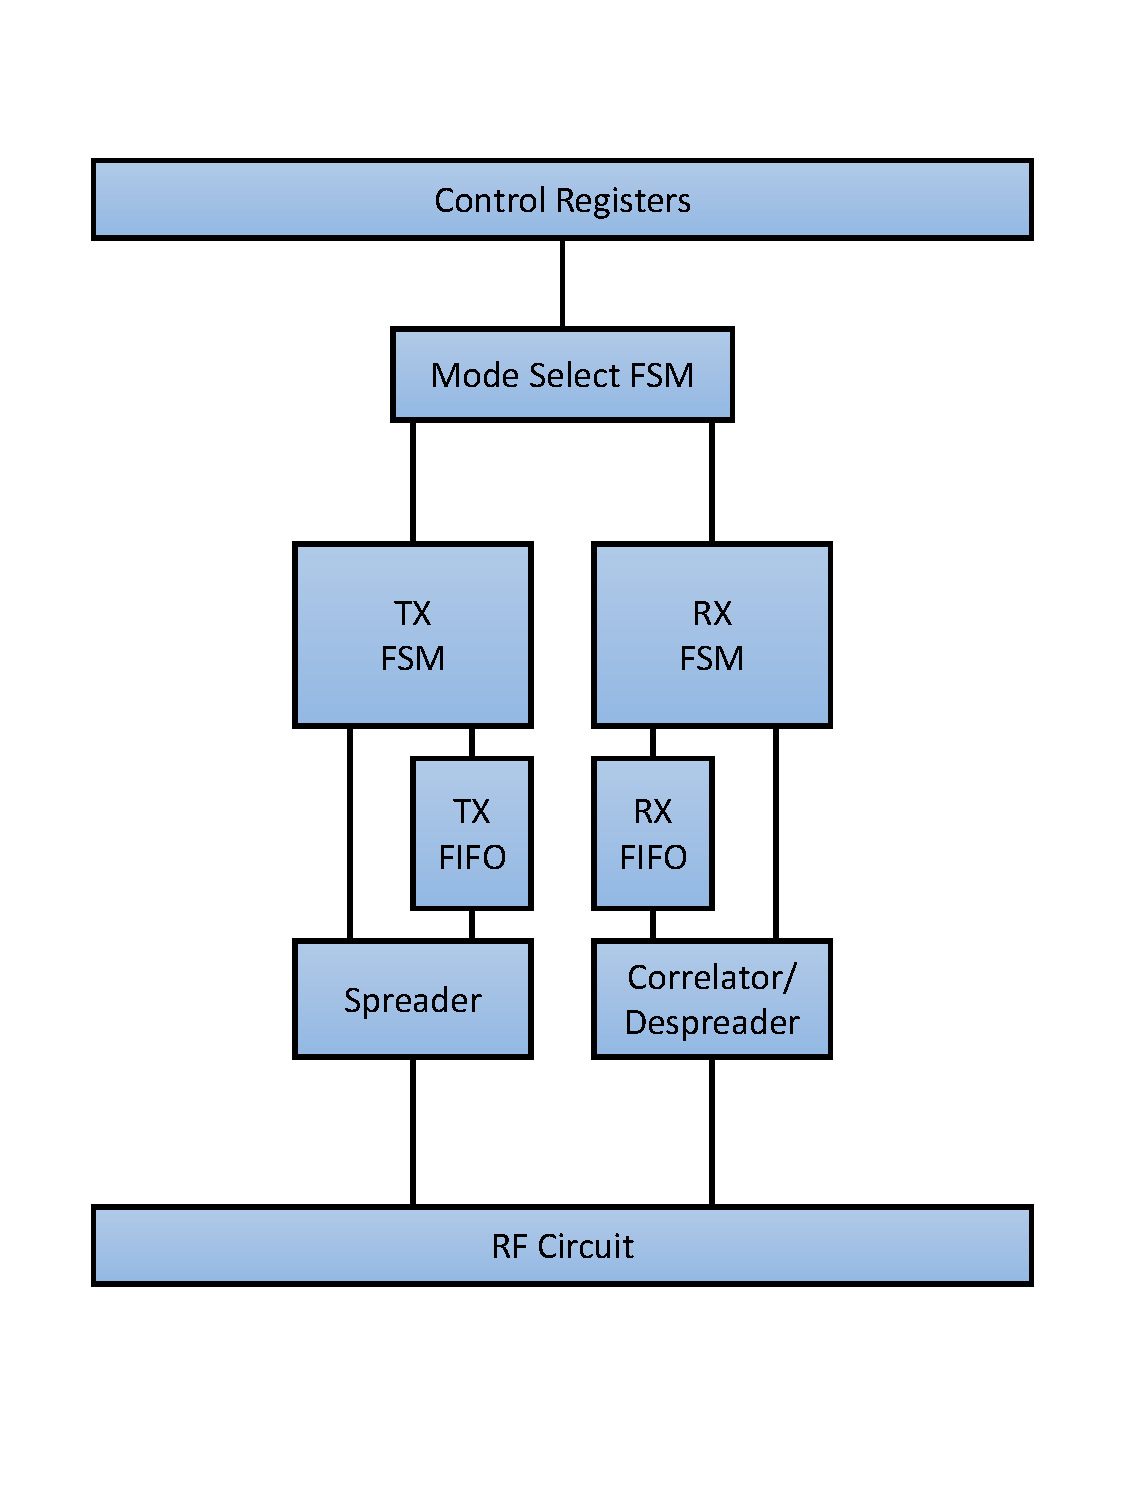
\includegraphics[width=0.7\linewidth]{rfcontroller-block-diagram}
\caption{Block diagram overview of the \texttt{RFcontroller} module and its connections to the radio circuit}
\label{fig:rfcontroller-block-diagram}
\end{figure}

\subsubsection{IEEE 802.15.4 Packets}
The radio circuit and \texttt{RFcontroller} module on the Single Chip Mote are designed to transmit and receive packets compliant with the IEEE 802.15.4 standard \cite{15-4-standard}. In particular, the radio circuit and \texttt{RFcontroller} module are responsible for implementing the physical (PHY) layer of the standard. This standard defines several different PHYs which use different frequency bands and modulation schemes. The Single Chip Mote implements the O-QPSK PHY, defined in section 10 of the standard.

The binary-encoded data in the packet is separated into groups of 4-bit symbols, where 2 symbols is equivalent to a byte. If the data is arranged in bytes then the least significant bits in a byte \texttt{[3:0]} make up the first symbol, and the most significant bits \texttt{7:4} make up the second symbol.

Each packet begins with a preamble, beginning with 8 copies of the \texttt{4'b0000} symbol. The preamble is followed by the 8-bit (2 symbol) start-of-frame delimiter (SFD).

Then follows the length of the packet payload, in bytes. This field is 7 bits wide (for a maximum payload length of 127 bytes), with 1 reserved bit to make it 8 bits (2 symbols) wide. Next is the payload, with an upper bound of 127 bytes. At the end of the packet is the 16-bit (4 symbol) cyclic redundancy check (CRC) value of the packet. Note that the length field includes the length of the payload but does \textit{not} include the preamble, SFD, length field, or CRC.

The binary data is not directly transmitted via the radio circuit. Instead, the binary data is converted from symbols to a serial bitstream of chips, and the chips modulate the transceiver on the radio circuit. The \texttt{RFcontroller} module operates on binary data; the \texttt{spreader} submodule converts symbols to chips for the radio circuit during transmission, and the \texttt{corr\_despreader} submodule converts received chips into symbols.

For more information, see the IEEE 802.15.4 standard \cite{15-4-standard}. A copy is also found in \path{scm-digital/doc/}.

\subsubsection{Finite State Machine Triggers}
This module uses three state machines to perform all of the functions required to send or receive packets. Both the TX and RX state machines are broken down into two major steps, each of which are initiated by the Cortex-M0 or the \texttt{RFTIMER} module via a particular trigger. The Cortex-M0 initiates these steps by setting the appropriate bit in the \texttt{RFCONTROLLER\_REG\_\_CONTROL} register. The \texttt{RFTIMER} module initiates these steps by asserting one of the \texttt{rftimer} inputs connected to this module. The four types of triggers are:

\begin{description}
	\item[\texttt{TX\_LOAD}] This trigger initiates the process of loading packet data into the TX FIFO for transmission.
	\item[\texttt{TX\_SEND}] This trigger initiates the process of sending the packet data in the TX FIFO to the radio circuit. This trigger has no effect if the FIFO is not currently loaded.
	\item[\texttt{RX\_START}] This trigger initiates the process of scanning the input data from the radio circuit to detect and process an incoming packet.
	\item[\texttt{RX\_STOP}] This trigger stops the process of detecting an incoming packet. This trigger has no effect if an incoming packet is already being processed.
\end{description}

These triggers are the only way for the software on the Cortex-M0 to control the radio circuit from a high level. All of the details are handled by the state machines and the \texttt{DMA\_V2} module.

\subsubsection{Mode Select Finite State Machine}
The mode select state machine shown in Figure \ref{fig:mode-fsm} is used to activate the TX and RX state machines when sending and receiving packets. The default state is \texttt{IDLE\_MODE}, where the radio is not sending or receiving packets.

The \texttt{TX\_LOAD} trigger, which comes from either setting the \texttt{TX\_LOAD} bit of the \texttt{RFCONTROLLER\_REG\_\_CONTROL} register or from the \texttt{RFTIMER} module, changes the state to \texttt{TX\_MODE}. When the transmission is finished, the state changes back to \texttt{IDLE\-\_MODE}. Setting the \texttt{RF\_RESET} bit of the \texttt{RFCONTROLLER\_REG\_\_CONTROL} register forces the state to change back to \texttt{IDLE\_MODE}.

The \texttt{RX\_START} trigger, which comes from either setting the \texttt{RX\_START} bit of the \texttt{RFCONTROLLER\_REG\_\_CONTROL} register or from the \texttt{RFTIMER} module, changes the state to \texttt{RX\_MODE}. When a packet is received, the state changes back to \texttt{IDLE\_MODE}. If there is no incoming packet, then setting the \texttt{RX\_STOP} bit of the \texttt{RFCONTROLLER\_REG\-\_\_CONTROL} register (or sending the \texttt{RX\_STOP} trigger from the \texttt{RFTIMER} module) changes the state back to \texttt{IDLE\_MODE}. \texttt{RX\_STOP} does not have an effect if the RX state machine is processing an incoming packet. Setting the \texttt{RF\_RESET} bit of the \texttt{RFCONTROLLER\_REG\_\_CONTROL} register forces the state to change back to \texttt{IDLE\_MODE}.

If both \texttt{TX\_LOAD} and \texttt{RX\_START} are triggered at the same time (either from the \texttt{RFCONTROLLER\_REG\_\_CONTROL} register or the \texttt{RFTIMER} module), \texttt{TX\_LOAD} takes precedence.

Figure \ref{table:modes} contains the state names and their binary encodings.

\begin{figure}
	\centering
	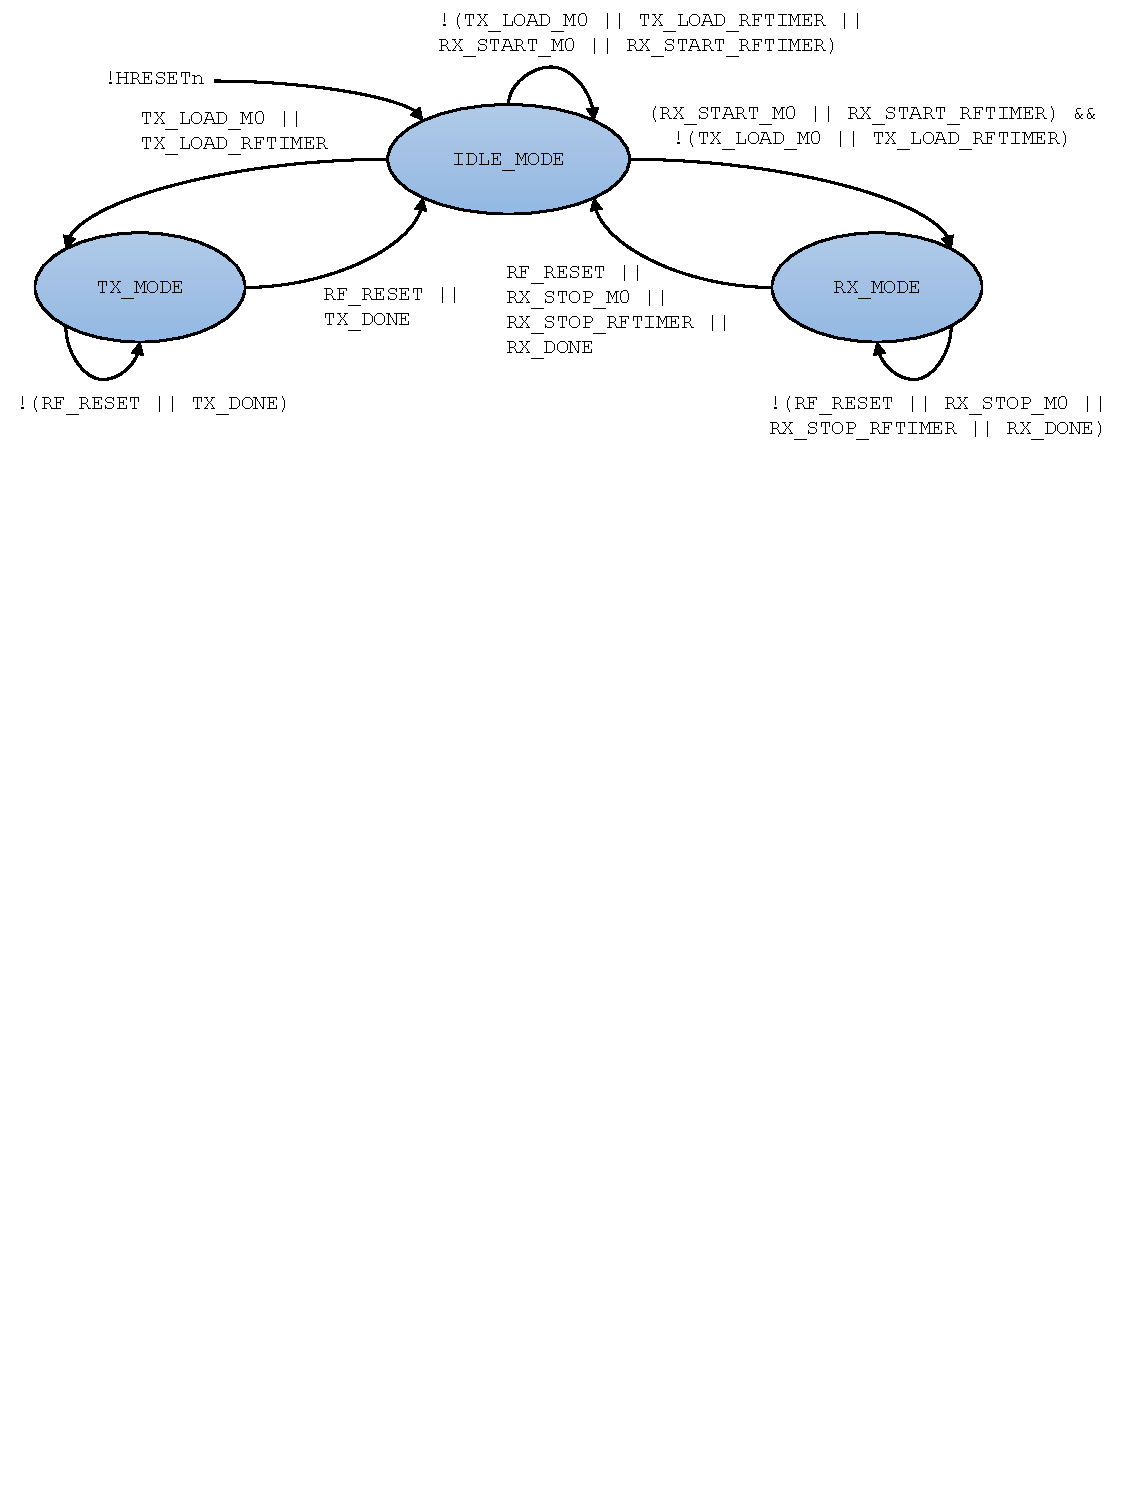
\includegraphics[width=1\linewidth]{mode-fsm}
	\caption{Mode select finite state machine for the \texttt{RFcontroller} module}
	\label{fig:mode-fsm}
\end{figure}

\begin{figure}
	\centering
	\begin{tabular}{|c|c|}
		\hline
		State Name & State Encoding [MSB:LSB] \\
		\hline
		\texttt{IDLE\_MODE} & \texttt{00} \\
		\texttt{TX\_MODE} & \texttt{01} \\
		\texttt{RX\_MODE} & \texttt{10} \\
		\hline
	\end{tabular}
	\caption{State encodings for the \texttt{RFcontroller} mode select FSM}
	\label{table:modes}
\end{figure}

\subsubsection{TX Finite State Machine}
The TX finite state machine shown in Figure \ref{fig:tx-fsm} performs all of the actions needed to transmit a packet. The TX FSM is activated when the mode changes to \texttt{TX\_MODE}. The FSM transitions through the following states and performs the following actions:

\begin{description}
	\item[\texttt{TX\_INIT}] Reset the TX FIFO, \texttt{spreader} module, and synchronizer modules. A request is sent to the \texttt{DMA\_V2} module for the first four bytes of data.
	\item[\texttt{TX\_INIT\_WAIT}] Wait for the \texttt{DMA\_V2} module to fetch the first four bytes of data. This also allows time for the FIFO to finish resetting.
	\item[\texttt{TX\_LOAD\_PHY}] Load the ten bytes of PHY layer headers for the packet into the FIFO. This includes the preamble, start symbol, and packet length.
	\item[\texttt{TX\_LOAD\_BYTE0/1/2/3}] Load byte 0/1/2/3 of the data fetched by the \texttt{DMA\_V2} module into the FIFO.
	\item[\texttt{TX\_DMA\_WAIT}] Wait for the \texttt{DMA\_V2} module to fetch the next four bytes of data.
	\item[\texttt{TX\_LOAD\_CRC0/1}] Load byte 0/1 of the CRC into the FIFO.
	\item[\texttt{TX\_LOAD\_DONE}] Assert the \texttt{TX\_LOAD\_DONE} interrupt. Wait for the \texttt{TX\_SEND} trigger to begin transmitting the packet.
	\item[\texttt{TX\_FIFO\_DRAIN}] Wait for all of the packet data to be read from the FIFO and transmitted via the \texttt{spreader} module. The \texttt{spreader} module also asserts the \texttt{TX\_SFD\_DONE} interrupt when the last bit of the SFD is sent.
	\item[\texttt{TX\_DONE}] Assert the \texttt{TX\_SEND\_DONE} interrupt. Reset the TX FIFO, \texttt{spreader} module, and synchronizer modules.
\end{description}

If the mode changes to \texttt{IDLE\_MODE} prematurely, either from an error or from \texttt{RF\_RESET}, the TX FSM transitions to the \texttt{TX\_DONE} state (in order to perform any necessary cleanup) and then to the default \texttt{TX\_SLEEP} state. Figure \ref{table:tx-states} contains the state names and their binary encodings. 

\begin{figure}
	\centering
	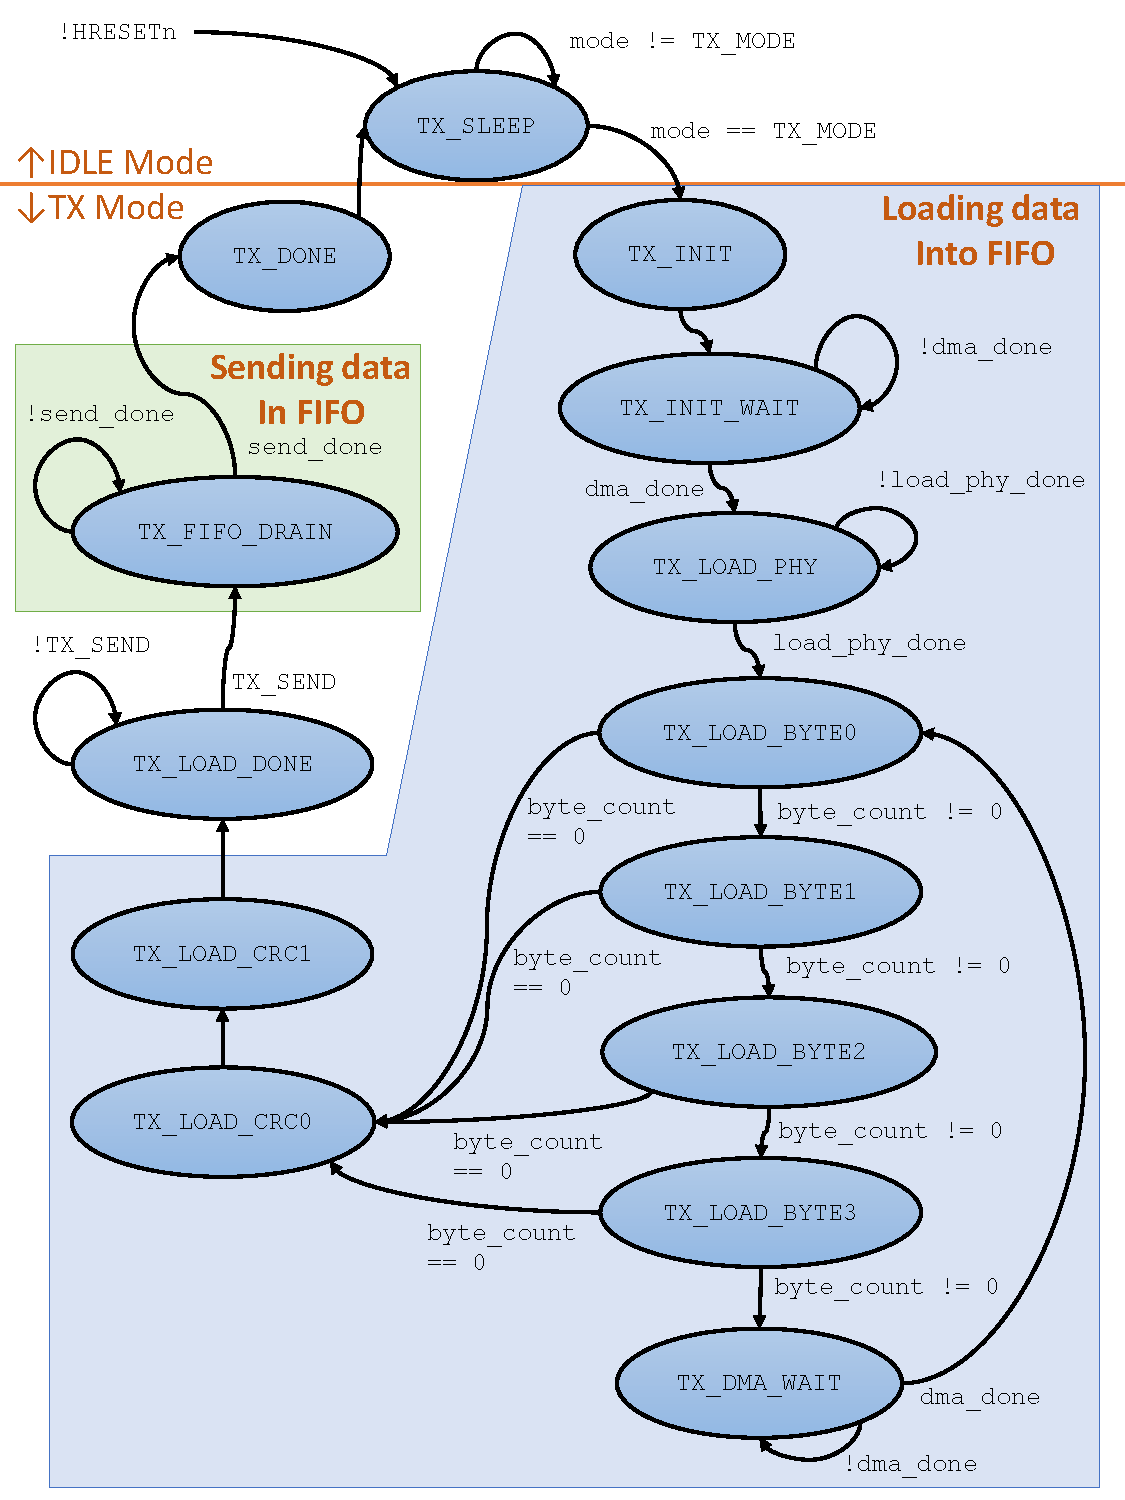
\includegraphics[width=1\linewidth]{tx-fsm}
	\caption{TX finite state machine for the \texttt{RFcontroller} module}
	\label{fig:tx-fsm}
\end{figure}

\begin{figure}
	\centering
	\begin{tabular}{|c|c|}
		\hline
		State Name & State Encoding [MSB:LSB] \\
		\hline
		\texttt{TX\_SLEEP} & \texttt{0000} \\
		\texttt{TX\_INIT} & \texttt{0011} \\
		\texttt{TX\_INIT\_WAIT} & \texttt{0010} \\
		\texttt{TX\_LOAD\_PHY} & \texttt{0110} \\
		\texttt{TX\_LOAD\_BYTE0} & \texttt{0111} \\
		\texttt{TX\_LOAD\_BYTE1} & \texttt{0101} \\
		\texttt{TX\_LOAD\_BYTE2} & \texttt{1100} \\
		\texttt{TX\_LOAD\_BYTE3} & \texttt{1101} \\
		\texttt{TX\_DMA\_WAIT} & \texttt{1111} \\
		\texttt{TX\_LOAD\_CRC0} & \texttt{0100} \\
		\texttt{TX\_LOAD\_CRC1} & \texttt{1110} \\
		\texttt{TX\_LOAD\_DONE} & \texttt{1010} \\
		\texttt{TX\_FIFO\_DRAIN} & \texttt{1000} \\
		\texttt{TX\_DONE} & \texttt{0001} \\
		\hline
	\end{tabular}
	\caption{State encodings for the \texttt{RFcontroller} TX FSM}
	\label{table:tx-states}
\end{figure}

\subsubsection{RX Finite State Machine}
The RX finite state machine shown in Figure \ref{fig:rx-fsm} performs all of the actions needed to listen for and receive a packet. The RX FSM is activated when the mode changes to \texttt{RX\_MODE}. The FSM transitions through the following states and performs the following actions:

\begin{description}
	\item[\texttt{RX\_INIT}] Reset the RX FIFO, \texttt{corr\_despreader} module, and synchronizer modules.
	\item[\texttt{RX\_GET\_LEN}] Wait for the \texttt{corr\_despreader} module to detect a packet. Once a packet has been detected, the \texttt{corr\_despreader} module provides the packet length and loads the packet data into the FIFO. The \texttt{corr\_despreader} module also asserts the \texttt{RX\_SFD\_DONE} interrupt when a packet is detected.
	\item[\texttt{RX\_GET\_BYTE0/1/2/3}] Read byte 0/1/2/3 from the FIFO.
	\item[\texttt{RX\_DMA\_WAIT}] Wait for the \texttt{DMA\_V2} module to finish storing the previous four bytes in memory.
	\item[\texttt{RX\_DATA\_STORE}] Signal the \texttt{DMA\_V2} module to store the current four bytes in memory.
	\item[\texttt{RX\_DMA\_WAIT2}] Wait for the \texttt{DMA\_V2} module to finish storying the last bytes of the packet in memory.
	\item[\texttt{RX\_CRC\_CHECK}] Check if the packet’s CRC is correct.
	\item[\texttt{RX\_DONE}]: Send the \texttt{RX\_DONE} interrupt. Reset the RX FIFO, \texttt{corr\_despreader} module, and synchronizer modules.
\end{description}

The RX finite state machine writes the packet data in the FIFO to the memory in the order that each byte is received. Preceding the packet data in memory is the length of the packet itself. Since the \texttt{DMA\_V2} module writes one word (four bytes) at a time to memory, the packet length is the least significant byte of the first word, and the rest of the packet data follows. This is accomplished by having the RX finite state machine transition to the \texttt{RX\_GET\_BYTE1} state (rather than \texttt{RX\_GET\_BYTE0}) when reading first byte of the packet data out of the RX FIFO. The last two bytes in the RX FIFO contain the CRC value of the packet, and this is also stored in memory after the packet data.

If the mode changes to \texttt{IDLE\_MODE} prematurely, either from an error or from \texttt{RF\_RESET}, the RX FSM transitions to the \texttt{RX\_DONE} state (in order to perform any necessary cleanup) and then to the default \texttt{RX\_SLEEP} state. Figure \ref{table:rx-states} contains the state names and their binary encodings. 

\begin{figure}
	\centering
	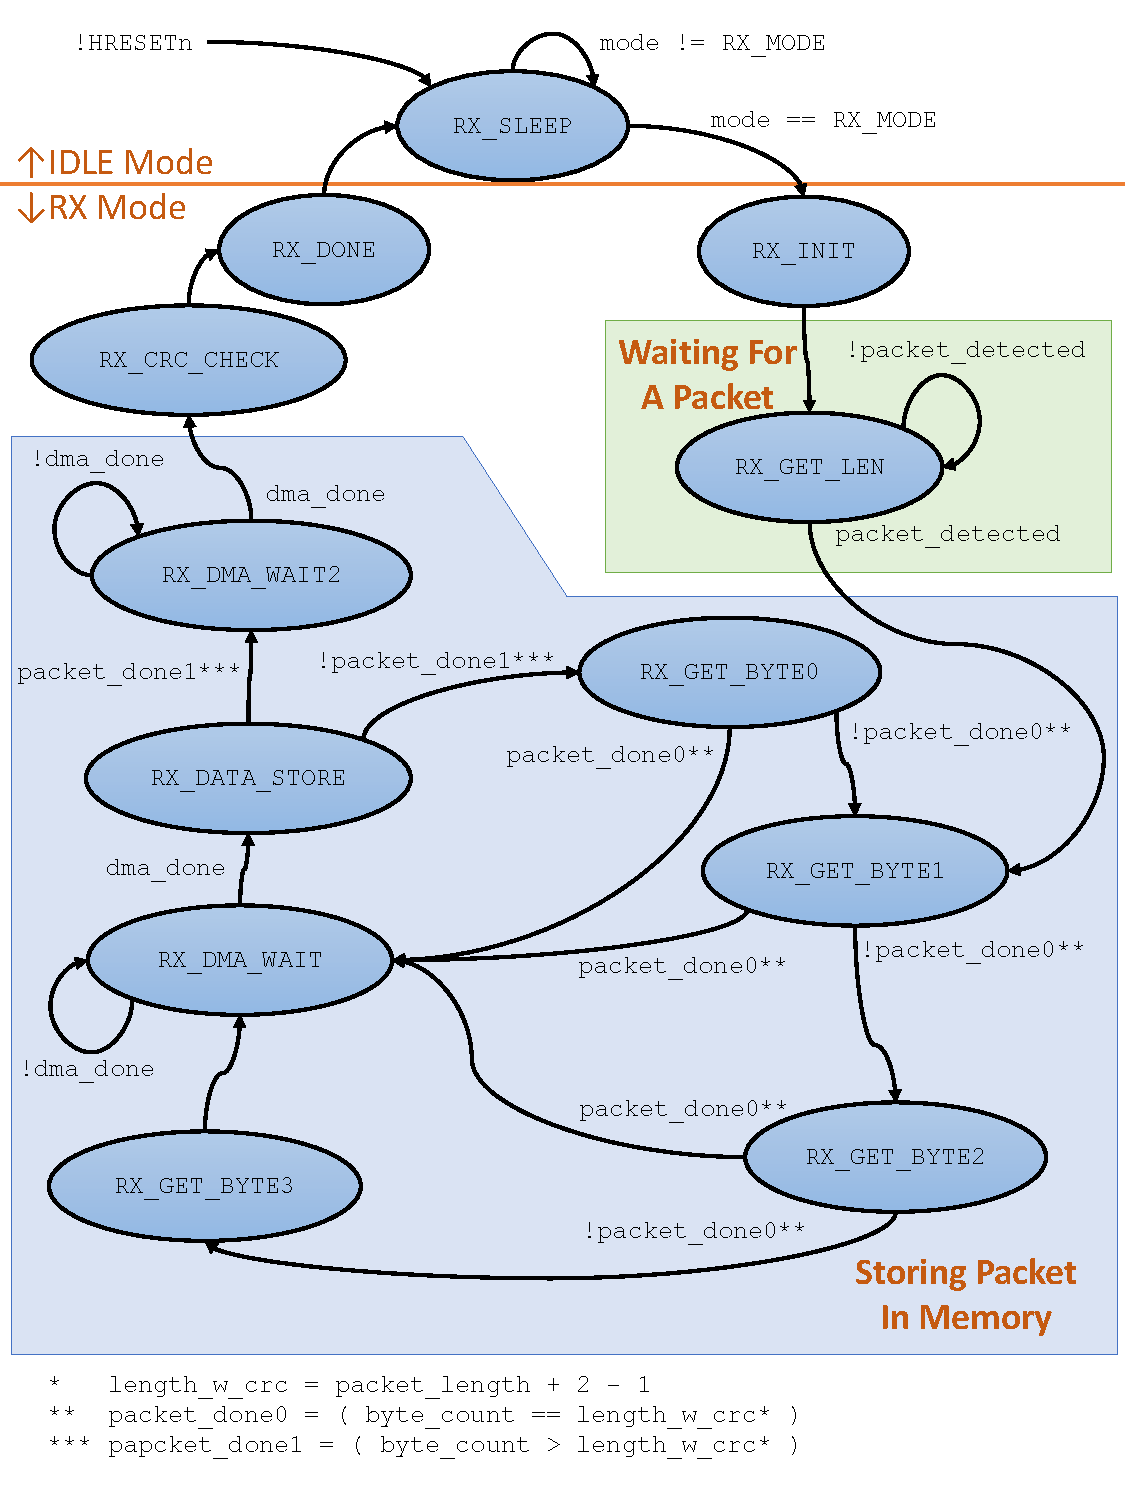
\includegraphics[width=1\linewidth]{rx-fsm}
	\caption{RX finite state machine for the \texttt{RFcontroller} module}
	\label{fig:rx-fsm}
\end{figure}

\begin{figure}
	\centering
	\begin{tabular}{|c|c|}
		\hline
		State Name & State Encoding [MSB:LSB] \\
		\hline
		\texttt{RX\_SLEEP} & \texttt{0000} \\
		\texttt{RX\_INIT} & \texttt{0011} \\
		\texttt{RX\_GET\_LEN} & \texttt{0010} \\
		\texttt{RX\_GET\_BYTE0} & \texttt{1111} \\
		\texttt{RX\_GET\_BYTE1} & \texttt{0111} \\
		\texttt{RX\_GET\_BYTE2} & \texttt{0110} \\
		\texttt{RX\_GET\_BYTE3} & \texttt{0100} \\
		\texttt{RX\_DMA\_WAIT} & \texttt{0101} \\
		\texttt{RX\_DATA\_STORE} & \texttt{1100} \\
		\texttt{RX\_DMA\_WAIT2} & \texttt{1101} \\
		\texttt{RX\_CRC\_CHECK} & \texttt{1110} \\
		\texttt{RX\_DONE} & \texttt{0001} \\
		\hline
	\end{tabular}
	\caption{State encodings for the \texttt{RFcontroller} RX FSM}
	\label{table:rx-states}
\end{figure}

\subsubsection{TX FIFO and Spreader}
The TX FIFO (found in the \texttt{tx\_fifo2} module) stores an entire packet, including headers and CRC, while it is waiting to be transmitted. The \texttt{TX\_LOAD} trigger enables the first part of the TX FSM. This part assembles the packet headers, packet data, CRC, and loads it all into the TX FIFO. The \texttt{TX\_SEND} trigger enables the second part of the TX FSM and the \texttt{spreader} module. This module reads the data out of the TX FIFO and encodes it into a sequence of chips that modulate the transceiver in the radio circuit to send the packet. Both of these modules are controlled by the TX FSM. See section \ref{tx-fifo} for more information on the \texttt{tx\_fifo2} module and section \ref{spreader} for more information on the \texttt{spreader} module.

\subsubsection{RX FIFO and Correlator/Despreader}
The RX FIFO (found in the \texttt{rx\_fifo} module) temporarily stores all received packet data and CRC after being decoded by the\texttt{corr\_despreader} module and before being stored into memory. The \texttt{RX\_START} trigger enables the RX FSM and also enables the \texttt{corr\_despreader} module. This submodule listens to the incoming chips from the radio circuit, and detects the SFD of a packet. Once this has been found, the \texttt{corr\_despreader} decodes the incoming chips back into binary data and stores it into the RX FIFO. At the same time, the RX FSM reads data out of the RX FIFO and stores it into memory. Both the RX FIFO and the \texttt{corr\_despreader} module are controlled by the RX FSM. See section \ref{rx-fifo} for more information on the \texttt{rx\_fifo} module and section \ref{corr-despreader} for more information on the \texttt{corr\_despreader} module.

\subsubsection{Clocking}
The \texttt{RFcontroller} module requires three separate clock domains in order to properly interface with the radio circuit. This is because the system clock (\texttt{HCLK}) used by the Cortex-M0 and all of the digital peripherals runs at 5MHz, and the radio circuit runs at 2MHz. The Single Chip Mote has a 2MHz source for transmitting packets called \texttt{CLK\_TX} in the top module and connected to the \texttt{tx\_clk} input to the \texttt{RFcontroller} module. The Single Chip Mote also has a separate 2MHz clock for receiving packets called \texttt{CLK\_RX} in the top module and connected to the \texttt{rx\_clk} input of the \texttt{RFcontroller} module. The RX clock comes from an analog circuit on the Single Chip Mote; this circuit generates a clock that is aligned with the incoming RX data.

Inside the \texttt{RFcontroller} module the control registers and the finite state machines use \texttt{HCLK}. The \texttt{spreader} module uses \texttt{tx\_clk} and the \texttt{corr\_despreader} module uses \texttt{rx\_clk}. The TX FIFO and RX FIFO are designed to be able to synchronize between separate clock domains and any additional cross-domain signals are properly synchronized using the \texttt{bit\_sync} and \texttt{bus\_sync} modules.

\subsubsection{DMA Interface}
The \texttt{RFcontroller} module relies on the \texttt{DMA\_V2} module to transfer packet data to and from the data memory. The \texttt{DMA\_V2} module is capable of reading and writing to the \texttt{RFcontroller} via the AHB bus. This is because the \texttt{DMA\_V2} module has an AHB master interface, and this interface shares the AHBsub bus with the Cortex-M0. Both the \texttt{DMA\_V2} module and the Cortex-M0 are AHB masters to the two AHB slaves on this shared bus: the \texttt{RFcontroller} module and the \texttt{AHBDMEM} module. The \texttt{RFcontroller} has two outputs connected directly to the \texttt{DMA\_V2} to send requests for data transfers over the AHB.

The \texttt{rf\_data\_req} output requests data from the memory for packet transmission. This output port is connected to the \texttt{txdatareq} register in the \texttt{RFcontroller} module. The \texttt{txdatareq} register is set by the TX FSM when it is time to fetch more data for transmission. The \texttt{DMA\_V2} module reads the \texttt{RFCONTROLLER\_REG\_\_TX\_DATA\-\_ADDR\_DMA} register to find the address of the data to fetch. Reading this register also clears the \texttt{txdatareq} register, as this read indicates that the \texttt{DMA\_V2} is servicing the request. The TX FSM waits for the \texttt{DMA\_V2} to write to the \texttt{RFCONTROLLER\_REG\_\_TX\-\_DATA\_DMA} register with the new packet data. This also causes the address stored in the \texttt{RFCONTROLLER\_REG\_\_TX\_DATA\_ADDR\_DMA} register to increment by 4.

The \texttt{rf\_data\_store} output requests that the \texttt{DMA\_V2} copy the received packet data in the \texttt{RFCONTROLLER\_REG\_\_RX\_DATA\_DMA} register to the data memory. 

The \texttt{rf\_data\_store} output is a register set by the RX FSM after the \texttt{RFCONTR\-O\-L\-L\-E\-R\-\_REG\_\_RX\_DATA\_DMA} is updated with new packet data. The \texttt{rf\_data\_store} register is cleared when the \texttt{DMA\_V2} reads from the \texttt{RFCONTR\-O\-L\-L\-E\-R\-\_REG\_\_RX\_DATA\_DMA} register, as this read indicates that the \texttt{DMA\_V2} is servicing the request.

In this case the \texttt{DMA\_V2} module, rather than the \texttt{RFcontroller} module, keeps track of where the new data is written, using the \texttt{DMA\_REG\_\_RF\_RX\_ADDR} register. The \texttt{DMA\_V2} module increments the address in \texttt{DMA\_REG\_\_RF\_RX\_ADDR} by 4 after every write.

For more information on the \texttt{DMA\_V2} module, see section \ref{dma}.

\subsubsection{Interrupts and Errors}
The \texttt{RFcontroller} has one interrupt to the Cortex-M0, as well as a register to indicate any errors. This single interrupt is a combination of several interrupt and error sources. This module also has a direct connection to the \texttt{RFTIMER} module to send interrupts (in the form of a single-cycle pulse) to any of its capture units (see section \ref{rftimer} spec for more details).

The five interrupt sources are:

\begin{description}
	\item[\texttt{TX\_LOAD\_DONE}] The TX FSM finishes copying packet data into the TX FIFO
	\item[\texttt{TX\_SFD\_DONE}] The spreader finishes transmitting the last bit of the packet’s SFD to the radio circuit
	\item[\texttt{TX\_SEND\_DONE}] The TX FSM finishes transmitting a packet
	\item[\texttt{RX\_SFD\_DONE}] The correlator/despreader detects an incoming packet
	\item[\texttt{RX\_DONE}] The RX FSM finishes receiving an incoming packet and storing the data into memory
\end{description}

The five error sources are:

\begin{description}
	\item[\texttt{TX\_OVERFLOW\_ERROR}] The TX FIFO overflows
	\item[\texttt{TX\_CUTOFF\_ERROR}] The TX FM is reset while a packet is sending
	\item[\texttt{RX\_OVERFLOW\_ERROR}] The RX FIFO overflows
	\item[\texttt{RX\_CRC\_ERROR}] The CRC of a received packet is incorrect (the packet data is still copied into memory)
	\item[\texttt{RX\_CUTOFF\_ERROR}] The RX FSM is reset while processing an incoming packet
\end{description}

Each of these interrupt or error sources correspond to a bit in the \texttt{RFCONTROLLER\-\_REG\_\_INT} or \texttt{RFCONTROLLER\_REG\_\_ERROR} registers. The \texttt{RFCONTROLLER\_REG\_\_INT\-\_CONFIG} and \texttt{RFCONTROLLER\_REG\_\_ERROR\_CONFIG} registers contain \texttt{INT\_EN} and \texttt{ER\-R\-OR\_EN} bits used to enable or disable each interrupt or error source. An enabled interrupt source sets the corresponding bit in the \texttt{RFCONTROLLER\_REG\_\_INT} register when the interrupt is triggered. A disabled interrupt source has no impact on the \texttt{RFCONTROLLER\_REG\_\_INT} register. The same applies to the error sources.

The Cortex-M0 interrupt is composed of the bitwise OR of the bits in the \texttt{RFCONTROLLER\_REG\_\_INT} and \texttt{RFCONTROLLER\_REG\_\_ERROR} registers, after they are masked by the \texttt{INT\_MASK} and \texttt{ERROR\_MASK} bits in the \texttt{RFCONTROLLER\_REG\_\_INT\-\_CONFIG} and \texttt{RFCON\-T\-R\-O\-L\-L\-E\-R\-\_REG\_\_ERROR\_CONFIG} registers. A masked bit in the \texttt{RFCONTROLLER\-\_REG\_\_INT} register means that it can be set but it will not trigger the Cortex-M0 interrupt. An unmasked bit will trigger the Cortex-M0 interrupt if it is set in the \texttt{RFCONTROLLER\_REG\_\_INT} register. The same applies to the bits in the \texttt{RFCONTROLLER\_REG\_\_ERROR} register.

In addition, each interrupt source is connected to the capture units of the \texttt{RFTIMER} module. Triggering the interrupt sends a single-cycle pulse to the \texttt{RFTIMER} module, if that interrupt source is enabled. This is set by the \texttt{PULSE\_EN} bits in the \texttt{RFCONTROLLER\_REG\_\_INT\_CONFIG} register. Error sources are not connected to the \texttt{RFTIMER} module

\subsection{Register Interface} \label{rfcontroller-registers}

\subsubsection{Control Register}
The \texttt{RFCONTROLLER\_REG\_\_CONTROL} register is a 5-bit register with fields that trigger parts of the TX and RX state machines. Its five bits are \texttt{TX\_LOAD}, \texttt{TX\_SEND}, \texttt{RX\_START}, \texttt{RX\_STOP}, and \texttt{RF\_RESET}.

The \texttt{TX\_LOAD} bit changes the mode from \texttt{IDLE\_MODE} to \texttt{TX\_MODE}, and launches the first part of the TX FSM responsible for loading packet data into memory. Once this is finished, the \texttt{TX\_SEND} bit launches the second part of the TX FSM, responsible for sending the packet through the radio circuit. After this is finished, the mode returns to \texttt{IDLE\_MODE}, and the TX state returns to \texttt{TX\_SLEEP}. Setting the \texttt{TX\_LOAD} bit has no effect when the mode is not \texttt{IDLE\_MODE}, and setting the \texttt{TX\_SEND} bit has no effect when the FIFO is not loaded (or in other words, the TX state is not \texttt{TX\_LOAD\_DONE}).

The \texttt{RX\_START} bit changes the mode from \texttt{IDLE\_MODE} to \texttt{RX\_MODE}, and launches the first part of the RX FSM responsible for listening for new packets. The \texttt{RX\_STOP} bit resets the RX state back to \texttt{RX\_SLEEP} and changes the mode back to \texttt{IDLE\_MODE}, under the condition that the \texttt{RFcontroller} module is not currently receiving a packet. Setting the \texttt{RX\_START} bit has no effect when the mode is not \texttt{IDLE\_MODE}, and setting the \texttt{RX\_STOP} bit has no effect when the radio is not listening for packets or is currently receiving a packet (or in other words, the RX state is not \texttt{RX\_GET\_LEN}).

The \texttt{RF\_RESET} bit resets all state machines back to their initial states in case of an unrecoverable error.

\subsubsection{Status Register}
The \texttt{RFCONTROLLER\_REG\_\_STATUS} register is a 10-bit register containing the current states of the three state machines. This register is used either to check the progress of sending/receiving a packet, or to check for any unexpected behavior (such as the FSM being ‘stuck’ in one state) for debugging purposes. This register contains two \texttt{MODE} bits for the state of the mode select FSM, four \texttt{TX\_STATE} bits for the TX FSM, and four \texttt{RX\_STATE} bits for the RX FSM. The encodings for each state are specified in Figures \ref{table:modes}, \ref{table:tx-states}, and \ref{table:rx-states}, respectively.

\subsubsection{TX Data Address and Packet Length}
The \texttt{RFCONTROLLER\_REG\_\_TX\_DATA\_ADDR} register is a 32-bit register containing the start address of the data to be transmitted. The address in this register must be word-aligned. All of the packet data must be in a continuous, sequential, word-aligned section of data memory beginning at the address stored in \texttt{RFCONTROLLER\-\_REG\-\_\_TX\_DATA\_ADDR}.

The \texttt{RFCONTROLLER\_REG\_\_PACK\_LEN} register is a 7-bit register containing the length of the data to be transmitted in bytes. The maximum data length, as defined by the IEEE 802.15.4 standard \cite{15-4-standard} is 127 bytes.

Both the \texttt{RFCONTROLLER\_REG\_\_TX\_DATA\_ADDR} and \texttt{RFCONTROLLER\_REG\_\_PACK\-\_LEN} registers must be updated before sending a packet to ensure that they point to the correct location in memory and indicate the correct length of the packet payload; however, their contents are not modified by the \texttt{RFcontroller} module during its operation.

\subsubsection{RX Data Address}
The \texttt{DMA\_REG\_\_RF\_RX\_ADDR} register is not part of the \texttt{RFcontroller} module; however, it must be updated before listening for a packet. This 32-bit register in the \texttt{DMA\_V2} module contains the starting address where received data is stored (see section \ref{dma} for more details). This address must refer to a continuous, word-aligned section of data memory designated in the software, with a length of at least 130 bytes, in order to be able to store the largest possible packet (127 bytes) and three additional bytes for the packet length and CRC. The address stored in \texttt{DMA\_REG\_\_RF\_RX\_ADDR} is modified by the \texttt{DMA\_V2} module while receiving a packet, and therefore must be set back to the correct value before listening for another packet. 

\subsubsection{DMA Exclusive Registers}
The following registers are part of the \texttt{RFcontroller} module, but are not meant to be accessed by the software running on the Cortex-M0. These registers are used by the \texttt{DMA\_V2} module to transfer packet data between the \texttt{RFcontroller} module and the data memory.

The \texttt{RFCONTROLLER\_REG\_\_TX\_DATA\_ADDR\_DMA} register is a 32-bit register containing the address of the next 4 bytes of data the \texttt{DMA\_V2} module must fetch for a packet transmission. The TX FSM copies the contents of the \texttt{RFCONTROLLER\_REG\-\_\_TX\_DATA\_ADDR} register into this register before loading the TX FIFO, and increments the contents of this register by 4 every time the \texttt{DMA\_V2} fetches new data.

The \texttt{RFCONTROLLER\_REG\_\_TX\_DATA\_DMA} register is a 32-bit register written by the \texttt{DMA\_V2} module with the data fetched for a packet transmission. The contents of this register are copied into the TX FIFO.

The \texttt{RFCONTROLLER\_REG\_\_RX\_DATA\_DMA} register is a 32-bit register containing the received packet data that the \texttt{DMA\_V2} copies into the FIFO. The RX FSM updates this value with new packet data and the \texttt{DMA\_V2} module reads this register and copies the contents to the data memory.

\subsubsection{Interrupt and Error Registers}
The \texttt{RFCONTROLLER\_REG\_\_INT} register is a 5-bit register indicating any interrupts from the \texttt{RFcontroller} module. The five bits correspond to the five types of interrupts: \texttt{TX\_LOAD\_DONE}, \texttt{TX\_SFD\_DONE}, \texttt{TX\_SEND\_DONE}, \texttt{RX\_SFD\_DONE}, and \texttt{RX\_DONE}. These bits are set if the interrupt is triggered and is enabled in the \texttt{RFCONTROLLER\-\_REG\-\_\_INT\_CONFIG} register. These bits are cleared by writing to the \texttt{RFCONTROLLER\-\_REG\-\_\_INT\-\_CLEAR} register.

The \texttt{RFCONTROLLER\_REG\_\_INT\_CONFIG} register is a 15-bit register containing the configuration flags for each interrupt source. The five \texttt{INT\_EN} bits enable or disable each interrupt source. An enabled interrupt source sets its corresponding bit in \texttt{RFCONTROLLER\_REG\_\_INT} when it is triggered, and a disabled interrupt source has no effect. The five \texttt{PULSE\_EN} bits enable or disable the pulse sent to the \texttt{RFTIMER} module for each interrupt source. An interrupt with a set \texttt{PULSE\_EN} bit sends a single-cycle pulse to the \texttt{RFTIMER} module when it is triggered. The five \texttt{INT\_MASK} bits determine whether or not the corresponding bit in \texttt{RFCONTROLLER\_REG\_\_INT} triggers the Cortex-M0 interrupt. An interrupt source with a set \texttt{INT\_EN} bit and a set \texttt{INT\_MASK} bit will set the corresponding bit in \texttt{RFCONTROLLER\_REG\_\_INT} when it triggers, but it will not trigger an interrupt to the Cortex-M0. Clearing the \texttt{INT\_MASK} bit while the corresponding bit in \texttt{RFCONTROLLER\_REG\_\_INT} is still set triggers a Cortex-M0 interrupt. 

The \texttt{RFCONTROLLER\_REG\_\_INT\_CLEAR} register is a 5-bit register that clears the bits in \texttt{RFCONTROLLER\_REG\_\_INT}. Setting any bit in this register to 1 clears the corresponding bit in \texttt{RFCONTROLLER\_REG\_\_INT}. Any unmasked bits set in the \texttt{RFCON\-T\-R\-O\-L\-L\-E\-R\-\_REG\_\_INT} register trigger the Cortex-M0 interrupt and a call to the interrupt service routine. The interrupt service routine must clear any unmasked bits (or mask them); otherwise, the ISR will execute again until all unmasked bits are cleared.

The \texttt{RFCONTROLLER\_REG\_\_ERROR} register is a 5-bit register indicating any errors from the \texttt{RFcontroller} module. The five bits correspond to the five types of errors: \texttt{TX\_OVERFLOW\_ERROR}, \texttt{TX\_CUTOFF\_ERROR}, \texttt{RX\_OVERFLOW\_ERROR}, \texttt{RX\_CRC\_ERROR}, and \texttt{RX\_CUTOFF\_ERROR}. These bits are set if the error is triggered and is enabled in the \texttt{RFCONTROLLER\_REG\_\_ERROR\_CONFIG} register. These bits are cleared by writing to the \texttt{RFCONTROLLER\_REG\_\_ERROR\_CLEAR} register.

The \texttt{RFCONTROLLER\_REG\_\_ERROR\_CONFIG} register is a 10-bit register containing the configuration flags for each error source. The five \texttt{ERROR\_EN} bits enable or disable each error source. An enabled error source sets its corresponding bit in \texttt{RFCONTROLLER\_REG\_\_ERROR} when it is triggered, and a disabled error source has no effect. The five \texttt{ERROR\_MASK} bits determine whether or not the corresponding bit in \texttt{RFCONTROLLER\_REG\_\_ERROR} triggers the Cortex-M0 interrupt. An error source with a set \texttt{ERROR\_EN} bit and a set \texttt{ERROR\_MASK} bit will set the corresponding bit in \texttt{RFCONTROLLER\_REG\_\_ERROR} when it triggers, but this will not trigger an interrupt to the Cortex-M0. Clearing the \texttt{ERROR\_MASK} bit while the corresponding bit in \texttt{RFCONTROLLER\_REG\_\_ERROR} is still set triggers a Cortex-M0 interrupt. 

The \texttt{RFCONTROLLER\_REG\_\_ERROR\_CLEAR} register is a 5-bit register that clears the bits in \texttt{RFCONTROLLER\_REG\_\_ERROR}. Setting any bit in this register to 1 clears the corresponding bit in \texttt{RFCONTROLLER\_REG\_\_ERROR}. Any unmasked bits set in the \texttt{RFCONTROLLER\_REG\_\_ERROR} register trigger the Cortex-M0 interrupt and a call to the interrupt service routine. The interrupt service routine must clear any unmasked bits (or mask them); otherwise, the ISR will execute again until all unmasked bits are cleared.

\subsubsection{Register Descriptions}
\ExecuteMetaData[chapters/registers.tex]{rfcontroller-registers}

\section{tx\_fifo2} \label{tx-fifo}
\subsection{Description}
This module is an asynchronous, asymmetric FIFO designed to store packet data waiting to be transmitted in the \texttt{RFcontroller} module. This module is asynchronous since it has two different clock inputs for reading (2MHz \texttt{CLK\_TX}) and writing (5MHz \texttt{HCLK}), and is asymmetric since the read data width (4 bits) and write data width (8 bits) are different. This FIFO stores up to 265 bytes and is large enough to store a transmitted packet at its maximum size. The design is based on the one described in \cite{async-fifo}, with additional modifications to deal with the asymmetric read and write data widths.

\subsection{Input/Output Ports}
\begin{description}
	\item[\texttt{reset\_n}] Input reset.
	\item[\texttt{wr\_clk}] Input write clock. The write data and write enable signals must be synchronized to this clock. The full flag is synchronized to this clock.
	\item[\texttt{wr\_en}] Write enable input. When this input is 1, the data on \texttt{wr\_data} is written into the FIFO.
	\item[\texttt{wr\_data[7:0]}] Write data input. This is the data written into the FIFO.
	\item[\texttt{wr\_full}] FIFO full output. This indicates that the FIFO is full and cannot accept any more data. Any attempts to write into a full FIFO will fail and the data will be lost.
	\item[\texttt{rd\_clk}] Input read clock. The read data and read enable signals must be synchronized to this clock. The empty flag is synchronized to this clock.
	\item[\texttt{rd\_en}] Read enable input. When this input is 1, the next value in the FIFO is read to the \texttt{rd\_data} output on the next cycle.
	\item[\texttt{rd\_data[3:0]}] Read data output. This is the data read from the FIFO.
	\item[\texttt{rd\_empty}] FIFO empty output. This indicates that the FIFO is empty and is not able to read additional data. Any attempts to read from an empty FIFO will fail and invalid data will be present on \texttt{rd\_data}.
\end{description}

\subsection{Design Details}
\subsubsection{Original Design}
The original implementation in \cite{async-fifo} uses an asynchronous read and write pointer comparison technique to reduce the amount of synchronization flip-flops in the design. Another side-effect of this technique is the improved temporal accuracy of the \texttt{rd\_empty} and \texttt{wr\_full} outputs.

The traditional asynchronous FIFO design requires a shift register to sample the read pointer with the write clock, and another shift register to sample the write pointer with the read clock. A FIFO using 8-bit pointers and a shift register depth of 3 (since greater depths reduce the chances of synchronization errors), requires 48 flip-flops. There is also at least a 3 cycle delay before the full or empty signals to de-assert. In contrast, the method used in \cite{async-fifo} requires only 5 flip-flops and some extra combinational logic.

This method creates an asynchronous empty signal, where its rising edge aligned to the read clock and its falling edge aligned to the write clock. A simple circuit containing two flip-flops solves this issue and synchronizes both edges to the read clock. This results in a \texttt{rd\_empty} signal that asserts as soon as the FIFO is empty, and de-asserts on the next read clock edge after the FIFO is not empty. The full signal has its rising edge aligned to the write clock and its falling edge aligned to the read clock. The same two-flop circuit synchronizes both edges to the write clock, and the \texttt{wr\_full} signal asserts as soon as the FIFO is full, and de-asserts on the next write clock edge after the FIFO is not full.

For more information on this FIFO design, see \cite{async-fifo}. A copy is found in \path{scm-digital/doc/}.

\subsubsection{Read Data Order}
The original implementation in \cite{async-fifo} assumes that the read and write data widths are the same. However, the \texttt{RFcontroller} modules requires a FIFO with 8-bit writes and 4-bit reads. For every 8 bits written to the FIFO, the lower 4 bits, [3:0], are read out of the FIFO first, and the upper 4 bits, [7:4], are read out of the FIFO second.

\subsubsection{Pointer Comparison Modifications}
The original implementation in \cite{async-fifo} uses Gray code read and write address pointers instead of binary-encoded pointers. Using Gray code reduces the chance of comparison and synchronization errors. However, the implementation in \texttt{tx\_fifo2} requires asymmetric read and write data widths, resulting in different read and write address pointer sizes. Given that the read data width is half of the write data width, the read pointer requires one more bit over the write pointer.

Consider the n-bit read pointer \texttt{rd\_addr[n-1:0]} and the n-1-bit write pointer, \texttt{wr\_addr[n-2:0]}. If the pointers are binary-encoded, then the FIFO is be full after a write when \texttt{rd\_addr[n-1:1] == wr\_addr[n-2:0]},and empty after a read when \texttt{rd\_addr[n-1:0] == \{wr\_addr[n-2:0], 1'b0\}}. The empty comparison fails when applied to two Gray code pointers of different sizes. This is because the least significant bit of \texttt{rd\_addr} is sometimes 0 after two reads, and sometimes 1 after two reads. As a Grey code pointer increments, the least significant bit changes according to the following pattern: 0110 (as opposed to 0101 with a binary pointer). For the pointers in this design, the problem is fixed by changing \texttt{\{wr\_addr[n-2:0], 1'b0\}} to \texttt{\{wr\_addr[n-2:0], \textasciicircum wr\_addr\}}.

\subsubsection{FIFO Memory Modifications}
The memory used to store the FIFO data is designed to behave like a synchronous SRAM with a width of 8 bits and a depth of 256 bits. This SRAM is not instantiated; however, the syntax used in the Verilog code infers a synchronous SRAM.

The write data width is 8 bits; one word of the RAM is written during every write, and the write address width of the FIFO matches write address width of the RAM. The read data width is 4 bits; therefore, the most significant bits (\texttt{rd\_addr[8:1]}) of the read address are used to address the 8-bit word in the RAM containing the desired 4 bits. The least significant bit (\texttt{rd\_addr[0]}) is used to determine which set of 4 bits in the RAM is the correct output.

Grey code pointers further complicate the read handling. As a Grey code pointer increments, the least significant bit changes according to the following pattern: 0110 (as opposed to 0101 with a binary pointer). Therefore, sometimes \texttt{rd\_addr[0] == 0} means the lower 4 bits must be read, and sometimes it means the upper 4 bits must be read. This is determined based on the value of \texttt{\textasciicircum rd\_addr[8:1]}.

\subsubsection{Overflow and Underflow Handling}
The original implementation in \cite{async-fifo} does not detect or handle overflows and underflows. This implementation was modified to allow reads only when the FIFO is not empty (by using \texttt{rd\_en \&\& !rd\_empty} instead of only \texttt{rd\_en}) and writes only when the FIFO is not full (by using \texttt{wr\_en \&\& !wr\_full} instead of only \texttt{wr\_full}). The asynchronous pointer comparisons allow for the \texttt{rd\_empty} output to assert as soon as the FIFO is empty and the \texttt{wr\_full} output to assert as soon as the FIFO is full; this is required for the prevention of overflows and underflows.

\section{rx\_fifo} \label{rx-fifo}
\subsection{Description}
This module is an asynchronous, asymmetric, first word fall through (FWFT) FIFO designed to received packet data in the \texttt{RFcontroller} module. This module is asynchronous since it has two different clock inputs for reading (5MHz \texttt{HCLK}) and writing (2MHz \texttt{CLK\_RX}), and is asymmetric since the read data width (8 bits) and write data width (4 bits) are different. This FIFO stores up to 128 bytes, 2 bytes smaller than the maximum size of received packet data. However, the \texttt{RFcontroller} module reads data out of the FIFO as soon as it is written, and therefore it is highly unlikely that the FIFO will overflow. The design is based on the one described in \cite{async-fifo}, with additional modifications to deal with the asymmetric read and write data widths and the addition of first word fall through logic.

\subsection{Input/Output Ports}
\begin{description}
	\item[\texttt{reset\_n}] Input reset.
	\item[\texttt{wr\_clk}] Input write clock. The write data and write enable signals must be synchronized to this clock. The full flag is synchronized to this clock.
	\item[\texttt{wr\_en}] Write enable input. When this input is 1, the data on \texttt{wr\_data} is written into the FIFO.
	\item[\texttt{wr\_data[3:0]}] Write data input. This is the data written into the FIFO.
	\item[\texttt{wr\_full}] FIFO full output. This indicates that the FIFO is full and cannot accept any more data. Any attempts to write into a full FIFO will fail and the data will be lost.
	\item[\texttt{rd\_clk}] Input read clock. The read data and read enable signals must be synchronized to this clock. The empty flag is synchronized to this clock.
	\item[\texttt{rd\_en}] Read enable input. When this input is 1, the next value in the FIFO is read to the \texttt{rd\_data} output on the next cycle.
	\item[\texttt{rd\_data[7:0]}] Read data output. This is the data read from the FIFO.
	\item[\texttt{rd\_empty}] FIFO empty output. This indicates that the FIFO is empty and is not able to read additional data. Any attempts to read from an empty FIFO will fail and invalid data will be present on \texttt{rd\_data}.
\end{description}

\subsection{Design Details}
\subsubsection{Original Design}
The original implementation in \cite{async-fifo} uses an asynchronous read and write pointer comparison technique to reduce the amount of synchronization flip-flops in the design. Another side-effect of this technique is the improved temporal accuracy of the \texttt{rd\_empty} and \texttt{wr\_full} outputs.

The traditional asynchronous FIFO design requires a shift register to sample the read pointer with the write clock, and another shift register to sample the write pointer with the read clock. A FIFO using 8-bit pointers and a shift register depth of 3 (since greater depths reduce the chances of synchronization errors), requires 48 flip-flops. There is also at least a 3 cycle delay before the full or empty signals to de-assert. In contrast, the method used in \cite{async-fifo} requires only 5 flip-flops and some extra combinational logic.

This method creates an asynchronous empty signal, with its rising edge aligned to the read clock and its falling edge aligned to the write clock. A simple circuit containing two flip-flops solves this issue and synchronizes both edges to the read clock. This results in a \texttt{rd\_empty} signal that asserts as soon as the FIFO is empty, and de-asserts on the next read clock edge after the FIFO is not empty. The full signal has its rising edge aligned to the write clock and its falling edge aligned to the read clock. The same two-flop circuit synchronizes both edges to the write clock, and the \texttt{wr\_full} signal asserts as soon as the FIFO is full, and de-asserts on the next write clock edge after the FIFO is not full.

For more information on this FIFO design, see \cite{async-fifo}. A copy is found in \path{scm-digital/doc/}.

\subsubsection{Write Data Order}
The original implementation in \cite{async-fifo} assumes that the read and write data widths are the same. However, the \texttt{RFcontroller} modules requires a FIFO 4-bit writes and 8-bit reads. For every 8 bits read from the FIFO, the lower 4 bits, [3:0], are written to the FIFO first, and the upper 4 bits, [7:4], are written to the FIFO second.

\subsubsection{Pointer Comparison Modifications}
The original implementation in \cite{async-fifo} uses Gray code read and write address pointers instead of binary-encoded pointers. Using Gray code reduces the chance of comparison and synchronization errors. However, the implementation in \texttt{tx\_fifo2} requires asymmetric read and write data widths, resulting in different read and write address pointer sizes. Given that the write data width is half of the read data width, the read pointer requires one less bit than the write pointer.

Consider the n-1-bit read pointer \texttt{rd\_addr[n-2:0]} and the n-bit write pointer, \texttt{wr\_addr[n-1:0]}. If the pointers are binary-encoded, then the FIFO is be empty after a read when \texttt{rd\_addr[n-2:0] == wr\_addr[n-1:1]}, and full after a write when \texttt{\{rd\_addr[n-2:0], 1\'b0\} == wr\_addr[n-1:0]}. The full comparison fails when applied to two Gray code pointers of different sizes. This is because the least significant bit of \texttt{wr\_addr} is sometimes 0 after two writes, and sometimes 1 after two writes. As a Grey code pointer increments, the least significant bit changes according to the following pattern: 0110 (as opposed to 0101 with a binary pointer). For the pointers in this design, the problem is fixed by changing \texttt{\{rd\_addr[n-2:0], 1'b0\}} to \texttt{\{rd\_addr[n-2:0], \textasciicircum rd\_addr\}}.

\subsubsection{FIFO Memory Modifications}
The memory used to store the FIFO data is designed to behave like a synchronous SRAM with a width of 8 bits, a depth of 128 bits, and write enable signals for the upper and lower 4 bits of the word line. This SRAM is not instantiated; however, the syntax used in the Verilog code infers a synchronous SRAM.

The read data width is 8 bits; one word in the RAM is read for every read, and the read address width of the FIFO matches read address width in the RAM. The write data width is 4 bits; therefore, the most significant bits (\texttt{wr\_addr[7:1]}) of the write address are used to address corresponding the 8-bit word in the RAM. The least significant bit (\texttt{wr\_addr[0]}) is used to determine which set of 4 bits in the RAM to overwrite.

Grey code pointers further complicate the write handling. As a Grey code pointer increments, the least significant bit changes according to the following pattern: 0110 (as opposed to 0101 with a binary pointer). Therefore, sometimes \texttt{wr\_addr[0] == 0} means the lower 4 bits must be written, and sometimes it means the upper 4 bits must be written. This is determined based on the value of \texttt{\textasciicircum wr\_addr[7:1]}.

\subsubsection{Overflow and Underflow Handling}
The original implementation in \cite{async-fifo} does not detect or handle overflows and underflows. This implementation was modified to allow reads only when the FIFO is not empty (by using \texttt{rd\_en \&\& !rd\_empty} instead of only \texttt{rd\_en}) and writes only when the FIFO is not full (by using \texttt{wr\_en \&\& !wr\_full} instead of only \texttt{wr\_full}). The asynchronous pointer comparisons allow for the \texttt{rd\_empty} output to assert as soon as the FIFO is empty and the \texttt{wr\_full} output to assert as soon as the FIFO is full; this is required for the prevention of overflows and underflows.

\subsubsection{First Word Fall Through Handling}
The original implementation in \cite{async-fifo} is designed such that the next word to be read is copied to the \texttt{rd\_data} output 1 cycle after \texttt{rd\_en} is asserted. First word fall through (FWFT) FIFOs have the next word copied to the \texttt{rd\_data} output as soon as the first word is written to the FIFO and immediately after the previous word is read. Therefore, valid data is always on the \texttt{rd\_data} output (unless the FIFO is empty), and asserting \texttt{rd\_en} indicates that the controlling module is ready for the next data word.

The FWFT logic is implemented by modifying the read enable signal sent to the FIFO memory. The original implementation uses the \texttt{rd\_en} input to the module as the read enable for the memory. The modified implementation uses \texttt{rd\_en || async\_empty\_n}, where \texttt{async\_empty\_n} is a signal that is high when the FIFO is not empty, and low when the FIFO is empty. This signal is updated as soon as an empty FIFO is written, and this signal is also used to generate \texttt{rd\_empty}. The result is that the data is transferred to \texttt{rd\_data} at the same time as \texttt{rd\_empty} is updated, ensuring the correct behavior. 

\section{spreader} \label{spreader}
\subsection{Description}
This module is part of the TX state machine in the \texttt{RFcontroller} module. This module reads packet data out of the \texttt{tx\_fifo2} module 4 bits at a time, where each set of 4 bits is called a symbol. This module converts each symbol into to a series of 32-bit chips, also referred to as OQPSK codes, outputted serially to the radio circuit, via the \texttt{tx\_dout} output of the top module. The process of converting symbols to chips is also called spreading. The radio circuit uses these chips to control the frequency of the transmitted signal. This module also indicates when it has finished transmitting the start-of-frame delimiter (SFD) of the packet, and when it has finished transmitting the entire packet. This is used by the \texttt{RFcontroller} module to trigger interrupts to the Cortex-M0 or the \texttt{RFTIMER} module.

\subsection{Input/Output Ports}
\begin{description}
	\item[\texttt{clk}] Input clock.
	\item[\texttt{resetn}] Input reset. This is be connected to the global reset. It is also recommended that this module be reset between packet transmissions.
	\item[\texttt{tx\_dout[3:0]}] Input data from the TX FIFO.
	\item[\texttt{tx\_start}] Input from the \texttt{RFcontroller} module to trigger the symbol-to-chip conversion and transmission.
	\item[tx\_fifo\_empty] Input indicating that the FIFO is empty. This indicates that all packet data is transmitted and the transmission is complete.
	\item[tx\_rd\_en] Read enable output to the TX FIFO to request more data.
	\item[tx\_sfd\_sent] Output pulse indicating that the last bit of the SFD has been sent.
	\item[\texttt{chip\_dout}] Serial output stream of chips sent to the radio circuit. This is connected to the radio circuit via the \texttt{tx\_dout} output of \texttt{RFcontroller} and the top module.
	\item[\texttt{done}] Output pulse indicating that the last bit of the packet has been sent.
\end{description}

\subsection{Design Details}

\subsubsection{OQPSK vs. MSK Modulation.}
The IEEE 802.15.4 standard \cite{15-4-standard} defines the symbol-to-chip mapping according to a method of modulation called OQPSK, which assigns one code (a set of 32 chips) to each 4-bit symbol. The method of modulation used in the radio for the Single Chip Mote is called MSK. The MSK modulator generates a radio signal equivalent to one generated by an OQPSK modulator. 

This module instantiates the \texttt{symbol2chips} submodule to convert symbols into two sets of 16 OQPSK chips, called I and Q. I includes all of the even chips in the code, and Q includes all of the odd chips in the code. If a single code has 32 chips, labeled $c_0,c_1,c_2,...,c_{30},c_{31}$, then the I chips are $c_0,c_2,c_4,...,c_{28},c_{30}$ and the Q chips are $c_1,c_3,c_5,...,c_{29},c_{31}$. Another way to describe this is to say that $i_n=c_{2n}$ and $q_n=c_{2n+1}$. The I chips and Q chips for OQPSK modulation are combined in a particular way to generate 32 chips for MSK modulation.

Suppose the $n$th symbol in a packet is equivalent OQPSK chips $i_{0,n}...i_{15,n}$ and $q_{0,n}...q_{15,n}$ and MSK chips $m_{0,n}...m_{15,n}$, then the conversion between OQPSK and MSK is:

$$m_{0,n} = i_{0,n} \oplus q_{0,n}$$
$$m_{1,n} = !(i_{1,n} \oplus q_{0,n})$$
$$m_{2,n} = i_{1,n} \oplus q_{1,n}$$
$$m_{3,n} = !(i_{2,n} \oplus q_{1,n})$$
$$m_{4,n} = i_{2,n} \oplus q_{2,n}$$
$$...$$
$$m_{28,n} = i_{14,n} \oplus q_{14,n}$$
$$m_{29,n} = !(i_{15,n} \oplus q_{14,n})$$
$$m_{30,n} = i_{15,n} \oplus q_{15,n}$$
$$m_{31,n} = !(i_{0,n+1} \oplus q_{15,n})$$

Note that the last chip of symbol $n$ depends on symbol $n+1$. The method to convert between OQPSK and MSK is described in more detail in \cite{cadence-paper}.

\subsubsection{State Machine}
This module uses a state machine used to read symbols from the TX FIFO, convert it to sets of I chips and Q chips, combine I and Q to generate MSK chips, and send each MSK chip serially to the radio circuit in the correct order. The I chips and Q chips are stored in the 16-bit \texttt{I} and \texttt{Q} registers, which are updated during the appropriate time by the state machine. The \texttt{i\_ptr} and \texttt{q\_ptr} registers store pointers to individual bits within the \texttt{I} and \texttt{Q} registers, which are also incremented at the appropriate time by the state machine. The output, \texttt{chip\_dout}, is assigned to \texttt{(I[i\_ptr] \textasciicircum Q[q\_ptr]) \textasciicircum inv\_chip\_dout}, where \texttt{inv\_chip\_dout} indicates that the output must be inverted (this signal is also set by the state machine). The overall procedure for converting an entire packet to MSK chips is described by the following states:

\begin{description}
	\item[\texttt{IDLE}] Wait for the \texttt{tx\_start} signal, then go to the \texttt{WAIT} state.
	\item[\texttt{WAIT}] After the \texttt{tx\_start} signal, wait for the TX FIFO to have data (indicated by \texttt{!tx\_fifo\_empty}), then go to the \texttt{FIFO\_READ} state. Reset \texttt{i\_ptr} to \texttt{4'b1111} and \texttt{q\_ptr} to \texttt{4'b1110}.
	\item[\texttt{FIFO\_READ}] Assert the read enable signal for the TX FIFO, increment \texttt{q\_ptr} from \texttt{4'b1110} to \texttt{4'b1111}, and go to the \texttt{CHIP\_CONVERSION\_I} state. The data on the output of the FIFO updates during the following cycle. The FIFO output data is connected to the input of the \texttt{symbol2chips} module, which converts the data into I and Q chips.
	\item[\texttt{CHIP\_CONVERSION\_I}] Store the updated value of the I chips onto the \texttt{I} register, increment \texttt{i\_ptr} from \texttt{4'b1111} to \texttt{4'b0000}, and go to the \texttt{CHIP\_CONVERSION\_Q} state.
	\item[\texttt{CHIP\_CONVERSION\_Q}] Store the updated value of the Q chips onto the \texttt{Q} register, increment \texttt{q\_ptr} from \texttt{4'b1111} to \texttt{4'b0000}, and go to the \texttt{SHIFT\_WAIT\_I} state.
	\item[\texttt{SHIFT\_WAIT\_I}] Increment \texttt{i\_ptr}. If \texttt{i\_ptr} is less than \texttt{4'b1110}, go to the \texttt{SHIFT\_WAIT\_Q} state. Otherwise, go to the \texttt{FIFO\_READ} state if there is still data in the FIFO (\texttt{!tx\_fifo\_empty}) or go to the \texttt{FINISH\_Q} state if the FIFO is empty.
	\item[\texttt{SHIFT\_WAIT\_Q}] Increment \texttt{q\_ptr} and go back to the \texttt{SHIFT\_WAIT\_I} state.
	\item[\texttt{FINISH\_Q}] Increment \texttt{q\_ptr} from \texttt{4'b1110} to \texttt{4'b1111} and go to the \texttt{FINISH} state.
	\item[\texttt{FINISH}] Assert the \texttt{done} output and go to the \texttt{IDLE} state.
\end{description}

This process is implemented in the state machine shown in Figure \ref{fig:spreader-fsm}. Note that \texttt{i\_ptr} and \texttt{q\_ptr} are not reset to zero. Instead, the pointers are reset in order to ensure that the \texttt{CHIP\_CONVERSION\_I} and \texttt{CHIP\_CONVERSION\_Q} states output the 31st and 32nd chip while also updating the \texttt{I} and \texttt{Q} registers at the appropriate time. In particular, the \texttt{CHIP\_CONVERSION\_Q} state requires $i_{0,n+1}$ and $q_{15,n}$ to generate the proper value for $m_{31,n}$. This requires that \texttt{i\_ptr} is \texttt{4'b0000}, \texttt{q\_ptr} is \texttt{4'b1111}, register \texttt{I} is updated right after the \texttt{CHIP\_CONVERSION\_I} state, and register \texttt{Q} is updated right after the \texttt{CHIP\_CONVERSION\_Q} state. Working backwards from there determines the default/reset values for \texttt{i\_ptr} and \texttt{q\_ptr}.

Also not shown in Figure \ref{fig:spreader-fsm} is how the \texttt{tx\_sfd\_sent} output is generated. The \texttt{read\_count} register keeps track of the number of reads from the FIFO. The \texttt{SFD\_DONE\_CYCLE} local parameter defines the number of reads from the FIFO until \textit{the last bit of the SFD has been sent}. The IEEE 802.15.4 standard \cite{15-4-standard} indicates that the beginning of a packet is comprised of 8 copies of the \texttt{4'b0000} symbol, followed by the two SFD symbols. Therefore, there are 10 symbols in the FIFO that must be read, converted, and transmitted before the \texttt{tx\_sfd\_sent} output is pulsed. However, the last bit of the SFD is sent just after the 11th symbol is read from the FIFO, during the \texttt{CHIP\_CONVERSION\_Q} state. Therefore, the \texttt{SFD\_DONE\_CYCLE} parameter is set to 11, and the \texttt{tx\_sfd\_sent} output is pulsed when \texttt{(read\_count == SFD\_DONE\_CYCLE) \&\& (state == CHIP\_CONVERSION\_Q)}. The \texttt{read\_count} register stops incrementing after \texttt{read\_count == SFD\_DONE\_CYCLE + 1} to avoid wasting energy.

\begin{figure}
\centering
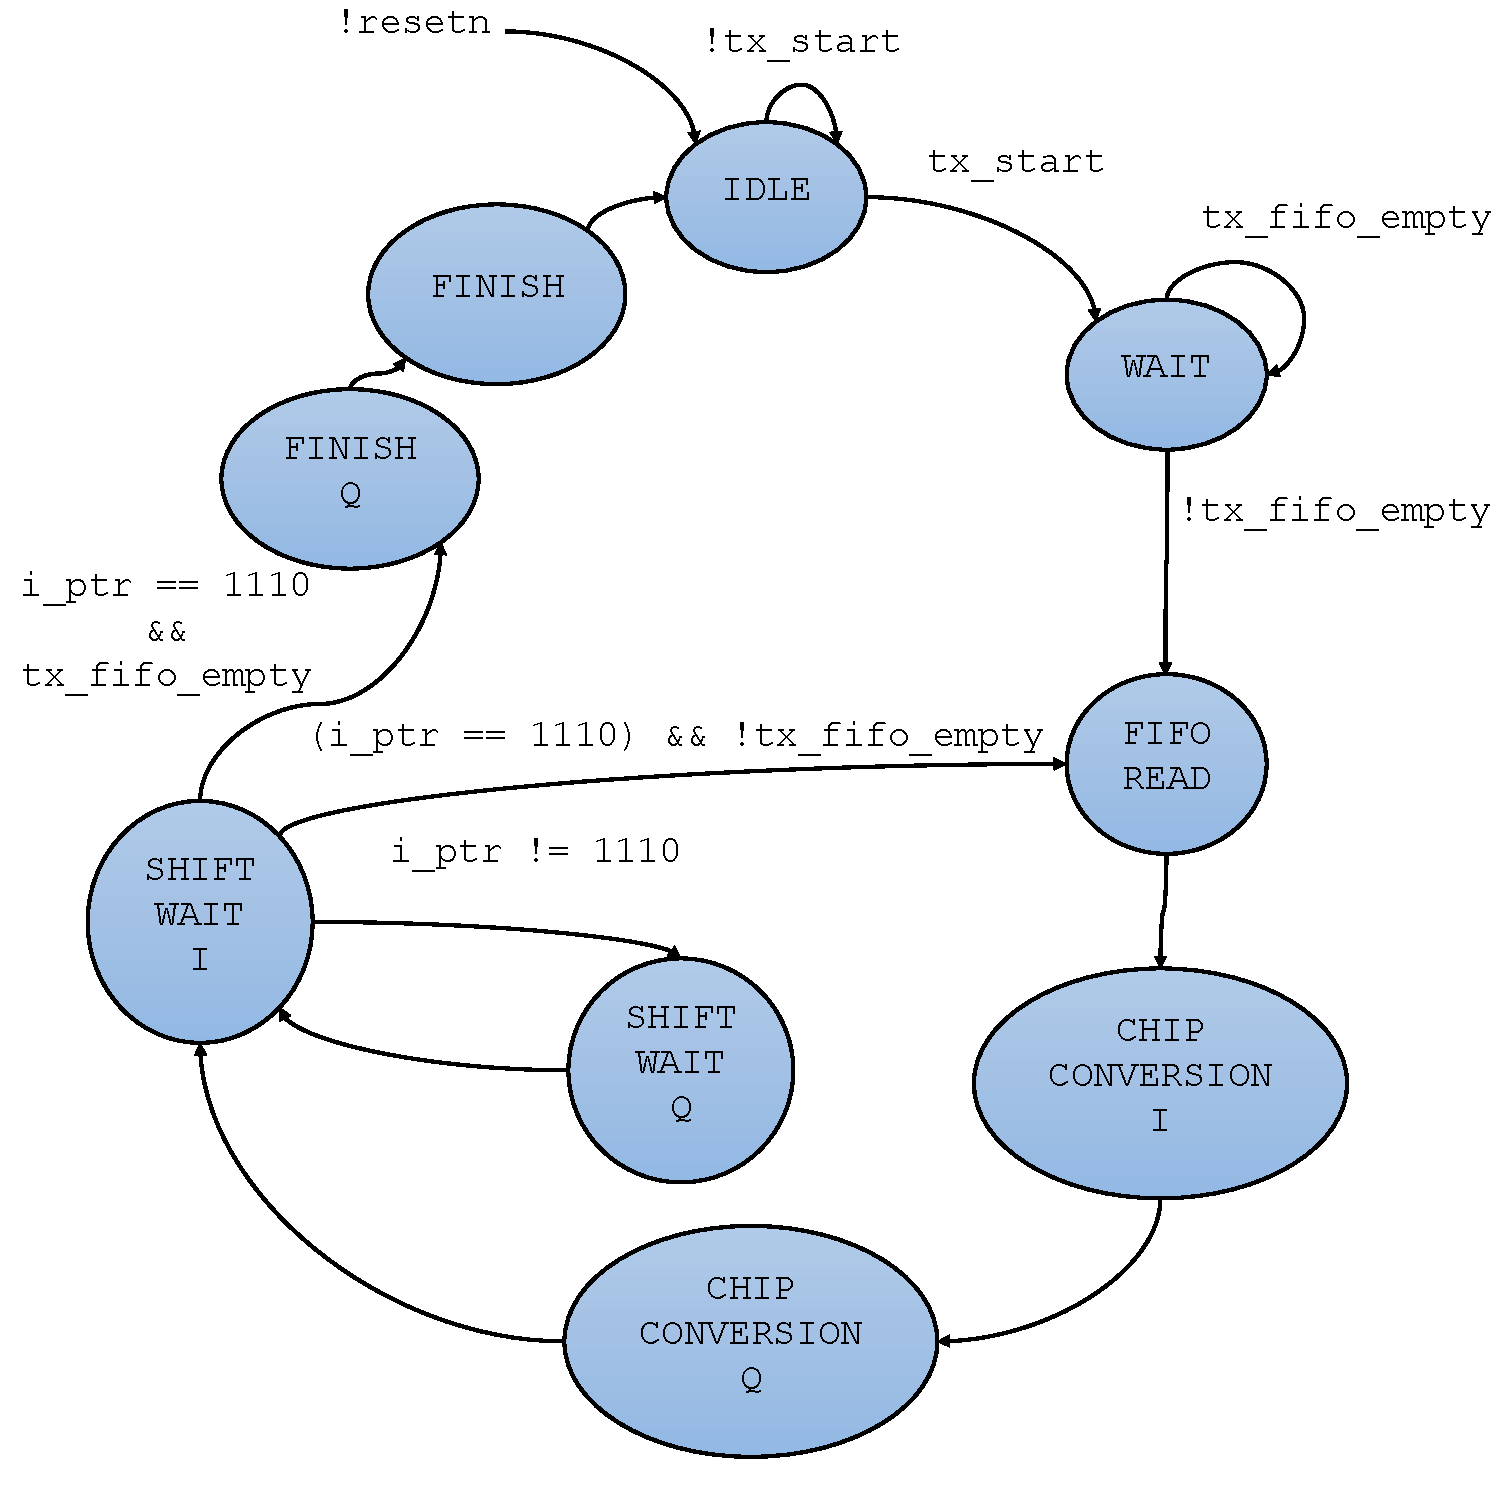
\includegraphics[width=1\linewidth]{spreader-fsm}
\caption{Finite State Machine for the \texttt{spreader} module}
\label{fig:spreader-fsm}
\end{figure}

\section{symbol2chips} \label{symbol2chips}
\subsection{Description}
This module contains the combinational logic needed in the \texttt{spreader} module to convert 4-bit symbols to two 16-bit sets of chips for radio packet data transmission. Each symbol has one set of chips called I and one set called Q. This module uses the \texttt{OQPSK\_I\_CODE} and \texttt{OQPSK\_Q\_CODE} values defined in \texttt{chips.vh} to map each symbol to a series of chips.

\subsection{Input/Output Ports}
\begin{description}
	\item[\texttt{symbol[3:0]}] Input symbol to be converted to chips.
	\item[\texttt{input\_valid}] Input indicating that the value on the \texttt{symbol} input is valid. When \texttt{input\_valid} is high, the output is also valid. When \texttt{input\_valid} is low, the input is ignored and the output corresponds to MSK code for the \texttt{4'b0000} symbol.
	\item[\texttt{I\_chips[15:0]}] Output containing the \texttt{OQPSK\_I\_CODE} corresponding to the input \texttt{symbol}. When \texttt{input\_valid} is low, the input is ignored and the output corresponds to the chips for the \texttt{4'b0000} symbol.
	\item[\texttt{Q\_chips[15:0]}] Output containing the \texttt{OQPSK\_Q\_CODE} corresponding to the input \texttt{symbol}. When \texttt{input\_valid} is low, the input is ignored and the output corresponds to the chips for the \texttt{4'b0000} symbol.
\end{description}

\subsection{Design Details}
This module implements a case statement used to select the correct OQPSK codes corresponding to the input symbol. The \texttt{input\_valid} input was added to multiplex the input to the combinational logic inside this module. This prevents any unnecessary switching when the module is not in use.

The IEEE 802.15.4 standard \cite{15-4-standard} defines the symbol-to-chip mapping for the particular frequency band used by the Single Chip Mote (2450MHz) in section 10.2.4. This section defines a set of 32 chips, $c_0...c_{31}$. The set I includes all of the even chips, $c_0,c_2,c_4,...,c_{28},c_{30}$, and the set Q includes all of the odd chips, $c_1,c_3,c_5,...,c_{29},c_{31}$. Another way to describe this is to say that $i_n=c_{2n}$ and $q_n=c_{2n+1}$. The Verilog file \url{chips.vh} contains the mapping for each 4-bit symbol to both I and Q.

\section{corr\_despreader} \label{corr-despreader}
\subsection{Description}
This module is part of the RX state machine in the \texttt{RFcontroller} module. This module reads the incoming data from the radio circuit in order to detect a received packet and store the data in the RX FIFO. The incoming data is a series of frequency shifts encoded into a serial binary data stream. These frequency shifts are determined using a demodulation circuit, and the Single Chip Mote uses a method of demodulation called MSK. The bits in the stream are called chips, and sets of 32 chips correspond to 4-bit sets of actual data called symbols. However, since this Single Chip Mote uses MSK demodulation, only the first 31 chips out of every set are used for comparison (see Dr. Osama Khan and Brad Wheeler for an explanation). This module scans the stream of chips to find the start of a packet, then converts the chips to symbols, and stores the symbols in the RX FIFO. This module also indicates when a packet has been detected to the \texttt{RFcontroller} module and provides the length of incoming packet to assist the RX state machine.

The process of converting chips to symbols is called despreading. Note that there are only 16 possible symbols, while there are $2^{32}$ possible combination of chips. Only 16 of those combinations correspond to symbols, and these combinations are referred to as MSK codes. If a packet is transmitted with no errors, then each set of 31 chips matches one of the 16 MSK codes. However, if there is an error in transmission, some of the chips may be changed. Therefore, this module must also take every input set of chips and find the closest matching code. This matching process is called correlation.

\subsection{Input/Output Ports and Parameters}
\begin{description}
	\item[\texttt{clk}] Input clock.
	\item[\texttt{resetn}] Input reset.
	\item[\texttt{rx\_din}] Serial input stream of chips from the radio circuit. This is connected to the radio circuit via the \texttt{rx\_din} input of the \texttt{RFcontroller} and top modules.
	\item[\texttt{rx\_start}] Input from the \texttt{RFcontroller} module indicating that this module begin scanning the \texttt{rx\_din} input to find the beginning of a packet.
	\item[\texttt{dout[3:0]}] Output symbols to be written to the RX FIFO.
	\item[\texttt{dout\_valid}] Output indicating that the data on \texttt{dout} is valid. This is the write enable input for the RX FIFO.
	\item[\texttt{packet\_detected}] Output indicating to the \texttt{RFcontroller} module that a packet has been detected. This output also indicates that the data on the \texttt{length} output is also valid.
	\item[\texttt{length[6:0]}] Output containing the length of the recently detected packet in bytes.
	\item[\texttt{THRESHOLD}] Parameter used when scanning the input data stream for the beginning of a packet. The beginning of a packet is indicated by a repeating set of symbols/chips called the preamble. This parameter determines how closely a set of chips must match the preamble chips before it is decided that a packet is detected. This parameter is passed into the \texttt{correlator} submodule.
\end{description}

\subsection{Design Details}
\subsubsection{Correlator}
This module instantiates the \texttt{correlator} submodule to find the symbol that is the closet match to the current set of chips, as well as quantify the `closeness' of that match. The `closeness' of a match is defined as the Hamming Distance, where a smaller Hamming Distance means a closer match, and a Hamming Distance of 0 indicates a perfect match. A minimum Hamming Distance threshold can be used when scanning for the start of a packet to reduce the amount of false-positives. This threshold is defined by the \texttt{THRESHOLD} parameter, also passed into the \texttt{correlator} submodule. Note that this module accepts 31 chips rather than 32 chips, since the last (most recent) chip cannot be used for correlation.

\subsubsection{Packet Detection}
The IEEE 802.15.4 standard \cite{15-4-standard} requires that the beginning of a packet is comprised of 8 copies of the \texttt{4'b0000} symbol, known as the preamble, followed by the two start-of-frame delimiter (SFD) symbols. The first SFD symbol (denoted in the code as \texttt{STARTSYMBOL0}) is \texttt{4'h0101} and the second SFD symbol (denoted in the code as \texttt{STARTSYMBOL1}) is \texttt{4'h1110}. The combination of the preamble and SFD are used to detect the beginning of a packet.

\subsubsection{Finite State Machine}
The input chip values are shifted each cycle into a 32-bit shift register. The procedure for detecting and capturing a packet is:

\begin{enumerate}
	\item Each time a new chip is shifted in, check if the closest matching symbol is \texttt{4'b0000}, and the minimum Hamming Distance is below the threshold.
	\begin{itemize}
		\item If the chips match \texttt{4'b0000}, part of the preamble, and the minimum Hamming Distance is below the threshold, wait 32 cycles for new chips to shift in and move on to the next step.
		\item If the chips do not match the preamble, or the minimum Hamming Distance is above the threshold, go back to the first step.
	\end{itemize}
	\item Check if the set of chips matches the preamble.
	\begin{itemize}
		\item If the chips match the preamble, wait 32 cycles for new chips to shift in and move on to the next step.
		\item If the chips do not match the preamble, go back to the first step.
	\end{itemize}
	\item Check if the set of chips matches the preamble or \texttt{STARTSYMBOL0}.
	\begin{itemize}
		\item If the chips match the preamble, wait 32 cycles for new chips to shift in and repeat this step.
		\item If the chips match \texttt{STARTSYMBOL0}, wait 32 cycles for new chips to shift in and move on to the next step.
		\item If the chips do not match the preamble or \texttt{STARTSYMBOL0}, go back to the first step.
	\end{itemize}
	\item Check if the set of chips matches \texttt{STARTSYMBOL1}.
	\begin{itemize}
		\item If the chips match \texttt{STARTSYMBOL1}, then a packet is detected. Wait 32 cycles for new chips to shift in and move on to the next step.
		\item If the chips do not match the preamble, go back to the first step.
	\end{itemize}
	\item The next two symbols contain the length of the packet in bytes. Store the first symbol, the LSB of the length. Wait 32 cycles.
	\item Store the next symbol, the MSB of the length.
	\item Use the packet length to determine how many symbols are left in the packet. Continue to wait 32 cycles between each symbol and store each symbol in the RX FIFO until the entire packet has been stored.
\end{enumerate}

This process is implemented in the state machine shown in Figure \ref{fig:corr-despreader-fsm}. The module stays in the \texttt{IDLE} state, where the input from the radio is ignored, until the \texttt{rx\_start} input is asserted by the \texttt{RFcontroller} module. The \texttt{SCAN} state is the first step, where the shift register is checked each cycle to see if it matches the preamble. The \texttt{PREAMBLE\_MATCH1} state is the second step, the \texttt{PREAMBLE\_MATCH2} state is the third step, and so on. The \texttt{max\_bit\_count} signal in Figure \ref{fig:corr-despreader-fsm} indicates when 32 new chips have been shifted into the shift register, and \texttt{max\_symbol\_count} indicates when all of the data in the packet has been copied into the RX FIFO.

Note that this state machine looks for two copies of the preamble symbol and then the beginning of the start symbol. The minimum number of preamble symbols is not adjustable in the current version of the Verilog code. This can be made adjustable by adding a counter and a parameter for the number of preamble symbols to the \texttt{PREAMBLE\_MATCH2} state. The parameterized counter can check for two or more preamble symbols in a row. To check for one preamble symbol, the \texttt{PREAMBLE\_MATCH2} state must be removed.

\subsubsection{Storing Packet Data Into the FIFO}
Each packet uses the two symbols after the SFD to indicate the size of the packet payload, in bytes. The length field is 7 bits wide, since the maximum payload length is 127 bytes. After the length is the packet payload, and after that there are two additional bytes containing the cyclic redundancy check (CRC) value of the packet. Both the payload and the CRC must be stored in the RX FIFO.

The \texttt{symbol\_count} register stores the number of symbols written into the FIFO. This register increments when the state is \texttt{PAYLOAD\_CAPTURE} and \texttt{max\_bit\_count == 1}, as this is when 32 new chips have been shifted in. At this point the chips are converted to a symbol and stored into the FIFO.  Once \texttt{symbol\_count} is equal to the number of symbols, minus one, and \texttt{max\_bit\_count == 1}, the last symbol is written to the FIFO and the state transitions back to \texttt{IDLE}. The \texttt{max\_symbol\_count} signal in Figure \ref{fig:corr-despreader-fsm} is not in the Verilog code, but it represents the code that checks if \texttt{symbol\_count} is equal to the number of symbols minus one.

\subsubsection{Calculating the Number of Symbols}
The first symbol after the SFD contains the LSB of the length, \texttt{length[3:0]}. The second symbol after the SFD contains the MSB of the length, \texttt{length[6:4]}. This length does not include the extra two bytes for the CRC. This means that the number of bytes to copy into the FIFO is \texttt{length[6:0] + 2}, and the number of symbols is twice as much.

Given that the value compared to \texttt{symbol\_count} is the number of symbols minus 1, the following simplifications allow for a small optimization in the size of the register storing this value:

$$ NumSymbolsInPacket = 2 \times (length + 2) $$
$$ NumSymbolsInPacket - 1 = 2 \times (length + 2) - 1 $$
$$ NumSymbolsInPacket - 1 = 2 \times (length + 1) + 2 - 1 $$
$$ NumSymbolsInPacket - 1 = 2 \times (length + 1) + 1 $$

In Verilog, this is the same as adding 1 to \texttt{length}, shifting to the left by one, and concatenating a 1 to the end, or \texttt{\{length+1, 1'b1\}}. Since the last bit is always 1, this module instead stores \texttt{length+1} in an 8-bit register called \texttt{total\_symbol\_count}, rather than the storing the actual number of symbols in the packet (requiring a 9-bit register). The state transitions from \texttt{PAYLOAD\_CAPTURE} to \texttt{IDLE} when \texttt{max\_bit\_count \&\& (symbol\_count == \{total\_symbol\_count, 1'b1\})}.


\begin{figure}
\centering
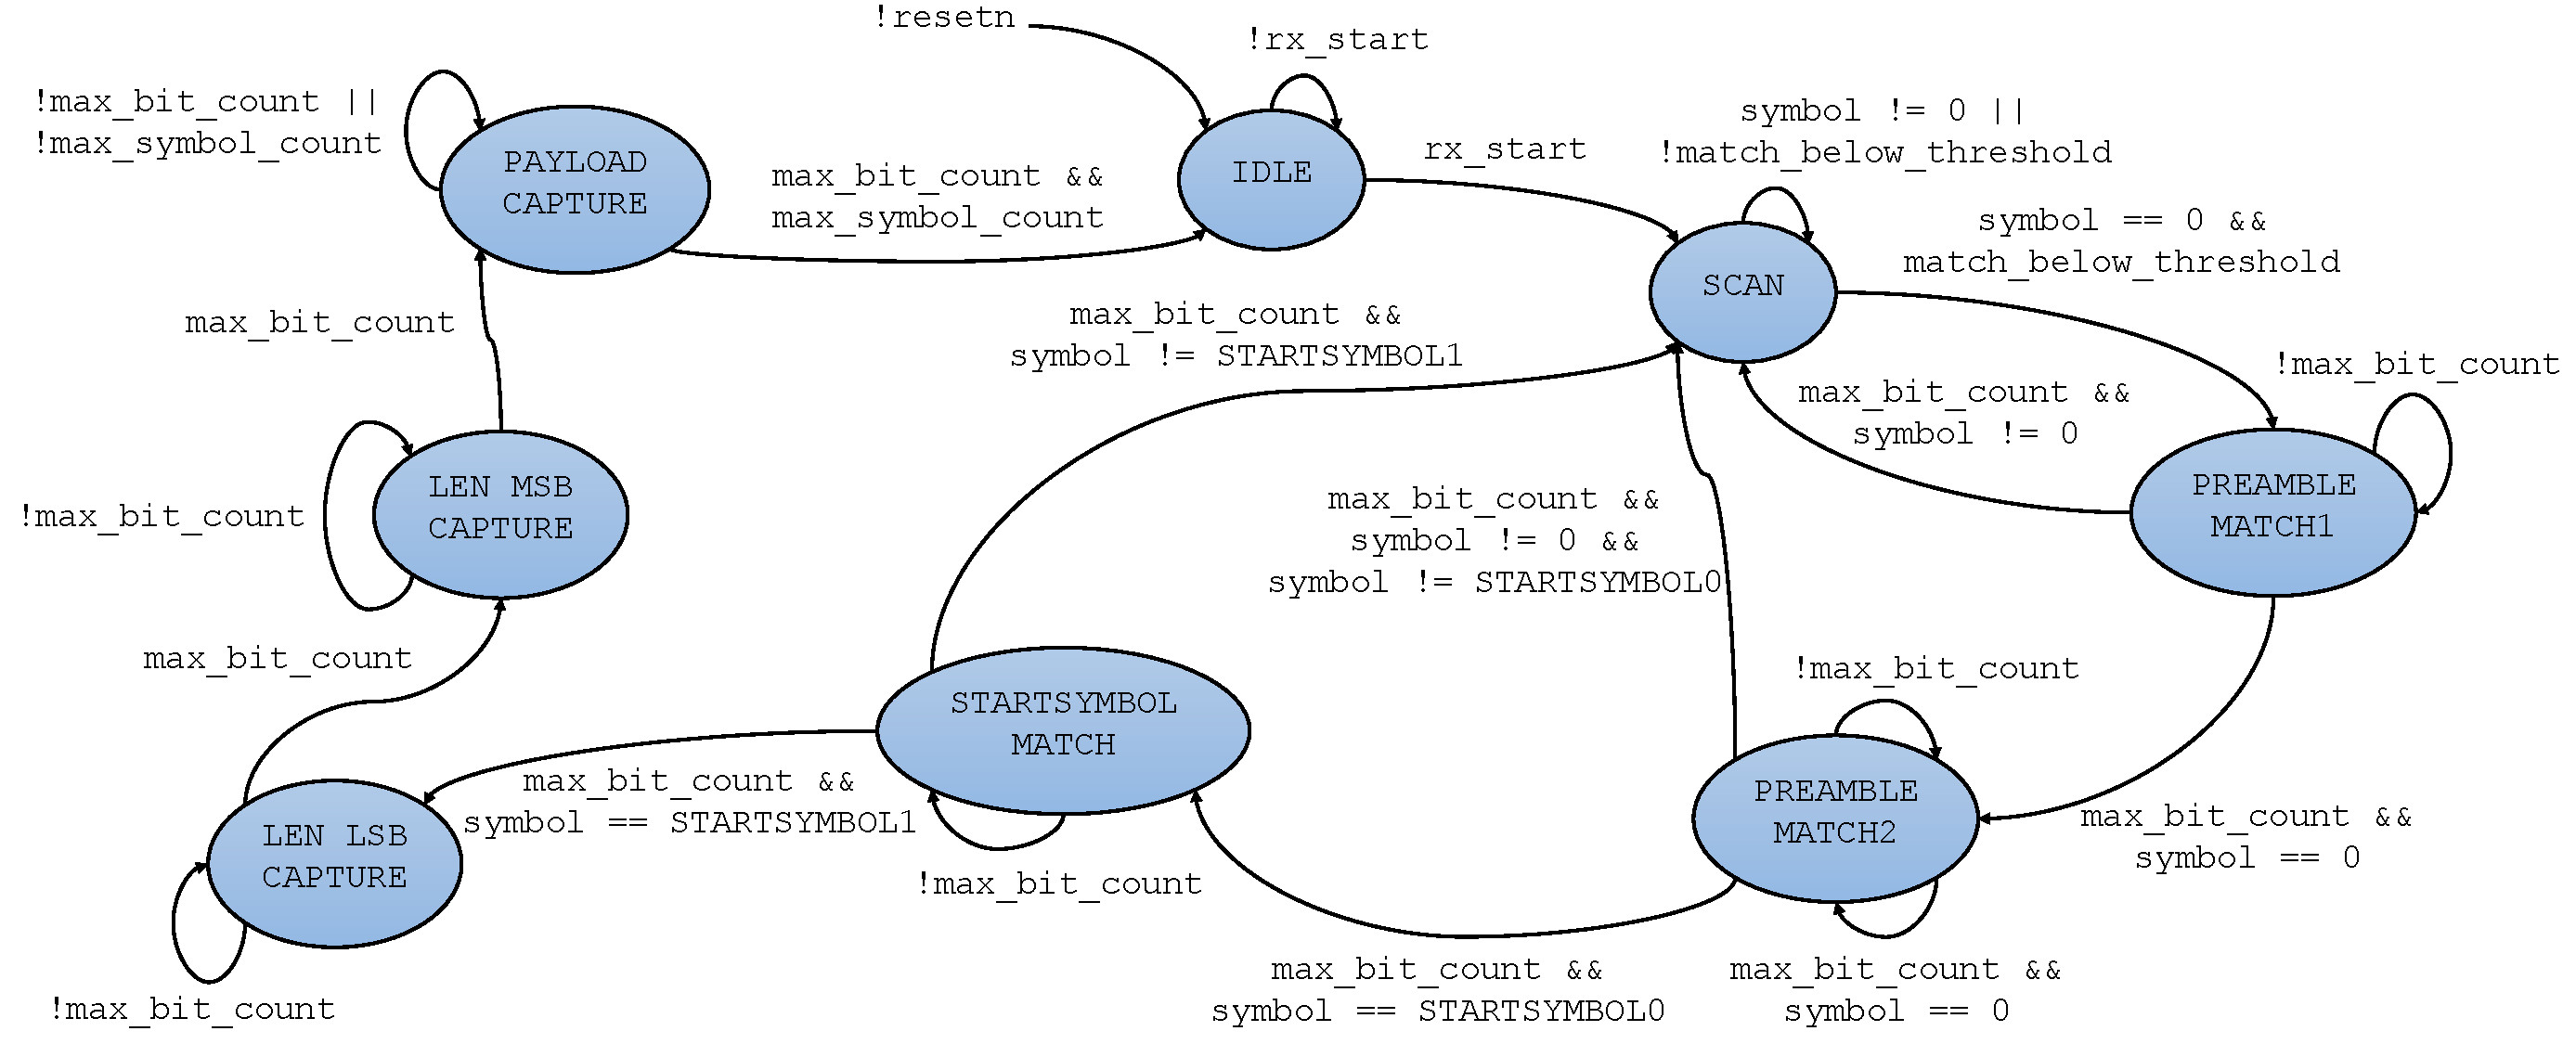
\includegraphics[width=\linewidth]{corr-despreader-fsm}
\caption{Finite State Machine for the \texttt{cor\_despreader} module}
\label{fig:corr-despreader-fsm}
\end{figure}

\section{correlator} \label{correlator}
\subsection{Description}
This module contains the combinational logic needed in the \texttt{corr\_despreader} module to find the 4-bit symbol that matches the current set of 31 chips. Each 4-bit symbol has a corresponding set of chips referred to as an MSK code. The Hamming Distance defines how 'close' two binary values are to one another, where a smaller Hamming Distance means a closer match, and a Hamming Distance of 0 means a perfect match. This module calculates the Hamming Distance between the input and each of the 16 possible MSK codes, and returns the symbol corresponding to the code with the minimum Hamming Distance. This module also has the option to check if the minimum Hamming Distance is at or below a threshold specified by a Verilog parameter. This threshold is used when the \texttt{corr\_despreader} module is scanning for the beginning of a packet.

\subsection{Input/Output Ports and Parameters}
\begin{description}
	\item[\texttt{chips\_in[30:0]}] 31-bit set of input chips to be correlated with a symbol.
	\item[\texttt{input\_valid}] Input indicating that the data on the \texttt{chips\_in} input is valid. When \texttt{input\_valid} is high, the output is also valid.
	\item[\texttt{use\_threshold}] Input indicating that the \texttt{correlator} module must also compare the calculated minimum Hamming Distance to the threshold specified by the \texttt{THRESHOLD} parameter. The result of this comparison is driven on the \texttt{match\_below\_threshold} output.
	\item[\texttt{symbol\_out[3:0]}] Output with the closest matching symbol to the \texttt{chips\_in} input. When \texttt{input\_valid} is low, the input is ignored and the output corresponds to the \texttt{4'b0000} symbol.
	\item[\texttt{match\_below\_threshold}] Output indicating that the current minimum Hamming Distance is at or below the threshold specified by the \texttt{THRESHOLD} parameter. This output is only valid when \texttt{use\_threshold} is high; otherwise, this output is 1.
	\item[\texttt{THRESHOLD}] Parameter describing the minimum Hamming Distance threshold used when scanning for the beginning of a packet.
\end{description}

\subsection{Design Details}
While the function of this module is seemingly simple, to find the minimum Hamming Distance between the input and a set of 16 codes and return the symbol corresponding to the code with the minimum distance, there is no straightforward method in Verilog to specify this behavior. The Verilog code for this module contains several generate statements to decrease the code size and take advantage of the redundancy in this design. As a result the code can be difficult to understand at first glance without a detailed explanation.

First, note that the MSK codes are all defined in the \texttt{chips.vh} header file. The mapping of symbols to MSK codes was provided by Brad Wheeler, a graduate student researcher working on the radio circuit for the Single Chip Mote. The following code copies these values into an array called \texttt{MSK\_CHIPS}, allowing for each individual code to be easily indexed within a generate statement:

\begin{lstlisting}
reg [30:0] MSK_CHIPS[0:15];
always @(*) begin
    MSK_CHIPS[0]  = `MSK_CODE_0;
    MSK_CHIPS[1]  = `MSK_CODE_1;
    MSK_CHIPS[2]  = `MSK_CODE_2;
    MSK_CHIPS[3]  = `MSK_CODE_3;
    MSK_CHIPS[4]  = `MSK_CODE_4;
    MSK_CHIPS[5]  = `MSK_CODE_5;
    MSK_CHIPS[6]  = `MSK_CODE_6;
    MSK_CHIPS[7]  = `MSK_CODE_7;
    MSK_CHIPS[8]  = `MSK_CODE_8;
    MSK_CHIPS[9]  = `MSK_CODE_9;
    MSK_CHIPS[10] = `MSK_CODE_A;
    MSK_CHIPS[11] = `MSK_CODE_B;
    MSK_CHIPS[12] = `MSK_CODE_C;
    MSK_CHIPS[13] = `MSK_CODE_D;
    MSK_CHIPS[14] = `MSK_CODE_E;
    MSK_CHIPS[15] = `MSK_CODE_F;
end
\end{lstlisting}

The following syntax specifies an array of registers: \texttt{reg [N-1:0] arr[0:M-1]}, where the \texttt{[N-1:0]} part indicates that the width of the registers is N bits, and the \texttt{[0:M-1]} part indicates that the number of registers in the array is M. In order to access these registers in Verilog, first the register must be selected, and then the bit(s) within the register are selected:

\begin{lstlisting}
reg [N-1:0] arr [0:M-1];
wire [N-1:0] myreg;
wire [2:0] mybits;

assign myreg = myarray[3];
assign mybits = myreg[2:0];
\end{lstlisting}

Several of these register arrays are used for the sections of this code written inside generate statements.

Calculating the Hamming Distance between two binary values is straightforward. The XOR of the two numbers returns another binary number with a 1 for each bit that does not match, and a 0 for every bit that does match. Adding the number of ones in this result yields the Hamming Distance. The \texttt{hamming\_distance\_xor} array holds the 31-bit results of XORing the input with each of the MSK codes. The \texttt{hamming\_distance\_sum} array holds the 5-bit results of adding the individual bits for each register in \texttt{hamming\_distance\_xor}. The values in \texttt{hamming\_distance\_sum} are equal to the Hamming Distance between the input and each of the MSK codes. This value ranges between 0 and 31. The calculation for these two arrays is found in the for loop labeled \texttt{calculate\_hamming\_distance}.

Finding the minimum Hamming Distance, and the corresponding symbol is much more difficult. The method used in this module is similar to performing a binary result on the values stored in the \texttt{hamming\_distance\_sum} array from the bottom-up.

The first step is to compare every two values in \texttt{hamming\_distance\_sum} and find the minimum. This means that \texttt{hamming\_distance\_sum[0]} is compared to \texttt{hamming\_distance\_sum[1]}, \texttt{hamming\_distance\_sum[2]} is compared to \texttt{hamming\-\_distance\_sum[3]}, and so on. The result of this comparison is eventually used to find the first bit of the \texttt{symbol\_out} output. The \texttt{bit0\_comparison\_result} register has 8 bits to store the results of this comparison in the following manner:

\begin{itemize}
	\item If \texttt{hamming\_distance\_sum[0] < hamming\_distance\_sum[1]}, then set\\ \texttt{bit0\_comparison\_result[0] = 1}. \\Otherwise, set \texttt{bit0\_comparison\_result[0] = 0}.
	\item If \texttt{hamming\_distance\_sum[2] < hamming\_distance\_sum[3]}, then set\\ \texttt{bit0\_comparison\_result[1] = 1}. \\Otherwise, set \texttt{bit0\_comparison\_result[1] = 0}.
	\item Continue following the same pattern until the results of all 8 comparisons are in \texttt{bit0\_comparison\_result}.
\end{itemize}

At the same time, the minimum Hamming Distances for each comparison are stored in the \texttt{bit0\_comparison\_minimum} arrays to be used for the next set of comparisons:

\begin{itemize}
	\item If \texttt{hamming\_distance\_sum[0] < hamming\_distance\_sum[1]}, then set\\ \texttt{bit0\_comparison\_minimums[0] = hamming\_distance\_sum[0]}. Otherwise, set \texttt{bit0\_comparison\_minimums[0] = hamming\_distance\_sum[1]}.
	\item If \texttt{hamming\_distance\_sum[2] < hamming\_distance\_sum[3]}, then set\\ \texttt{bit0\_comparison\_minimums[1] = hamming\_distance\_sum[2]}. Otherwise, set \texttt{bit0\_comparison\_minimums[1] = hamming\_distance\_sum[3]}.
	\item Continue following the same pattern until the minimum Hamming Distances of all 8 comparisons are in \texttt{bit0\_comparison\_minimums}.
\end{itemize}

The first set of comparisons, and the assignments to \texttt{bit0\_comparison\_result} and \texttt{bit0\_comparison\_minimums} is found in the for loop labeled \texttt{compare\_bit0}.

The next step is to compare every two values in \texttt{bit0\_comparison\_minimums}, and store those minimums. This is the same as the process described in the first set of comparisons, only now the \texttt{bit0\_comparison\_minimums} values are being compared, and the results are stored in \texttt{bit1\_comparison\_result} and \texttt{bit1\_comparison\_min\-i\-mums}. This time there are 4 comparisons in total, and the code is found in the for loop labeled \texttt{compare\_bit1}.

The third step is to compare every two values in \texttt{bit1\_comparison\_minimums}, and store those minimums. This is the same as the process described in the first set of comparisons, only now the \texttt{bit1\_comparison\_minimums} values are being compared, and the results are stored in \texttt{bit2\_comparison\_result} and \texttt{bit2\_comparison\_min\-i\-mums}. This time there are 2 comparisons in total, and the code is found in the for loop labeled \texttt{compare\_bit2}.

The final step is to compare the two values in \texttt{bit2\_comparison\_minimums} and store the result in the \texttt{bit3\_comparator} register. The following code essentially performs a binary search over the results stored in the \texttt{bit3\_co\-m\-parator} and \texttt{bitx\_comparison\_result} registers in order to find the symbol with the minimum distance:

\begin{lstlisting}
assign hamming_distance_minimum_symbol[3] = ~bit3_comparator;
assign hamming_distance_minimum_symbol[2] = ~bit2_comparison_result[hamming_distance_minimum_symbol[3]];
assign hamming_distance_minimum_symbol[1] = ~bit1_comparison_result[hamming_distance_minimum_symbol[3:2]];
assign hamming_distance_minimum_symbol[0] = ~bit0_comparison_result[hamming_distance_minimum_symbol[3:1]];
\end{lstlisting}
Finally, the following code assigns \texttt{symbol\_out}, and checks if the minimum distance is at or below the threshold:

\begin{lstlisting}
assign minimum_distance = hamming_distance_sum[hamming_distance_minimum_symbol];
assign match_below_threshold = use_threshold ? (minimum_distance <= THRESHOLD) : 1'b1;
assign symbol_out = hamming_distance_minimum_symbol;
\end{lstlisting}

\section{bit\_sync}
\subsection{Description}
This module synchronizes a signal from a slower clock domain to a faster one. In particular, the fast clock samples the signal from the slow clock, and outputs a single-cycle (according to the fast clock) pulse when a rising edge is detected.

This module is used in the \texttt{RFcontroller} module to synchronize the \texttt{tx\_sfd\-\_sent} and \texttt{tx\_spread\-\_done} signals from the \texttt{spreader} module. These signals indicate that the last bit of a packet's SFD and the last bit of a packet has finished transmitting, respectively.

\subsection{Input/Output Ports}
\begin{description}
	\item[\texttt{reset\_n}] Input reset.
	\item[\texttt{enable}] Enable input for the entire synchronizer. Inputs are only be sampled when this input is asserted. The output remains low unless this input is asserted.
	\item[\texttt{in}] Input signal to be sampled. This input must be aligned to a clock slower than \texttt{clk\_out}.
	\item[\texttt{clk\_out}] Input sampling clock. This clock is used to sample the input, \texttt{in}. The output pulse, \texttt{out}, is aligned to this clock.
	\item[\texttt{out}] Edge detected pulse output. This output is a single-cycle pulse (aligned with \texttt{clk\_out}) indicating that an edge in the \texttt{in} input is detected.
\end{description}

\subsection{Design Details}
This synchronizer is designed using a shift register of depth 4 to sample the input. A long shift register is used to reduce the probability of metastability at the output. The last two bits in the shift register are compared to determine if there is a rising edge in the input. The shift register does not sample new values unless the \texttt{enable} input is asserted, and the output remains low unless the \texttt{enable} input is asserted. A schematic of this circuit is shown in Figure \ref{fig:bit-sync}.

\begin{figure}
\centering
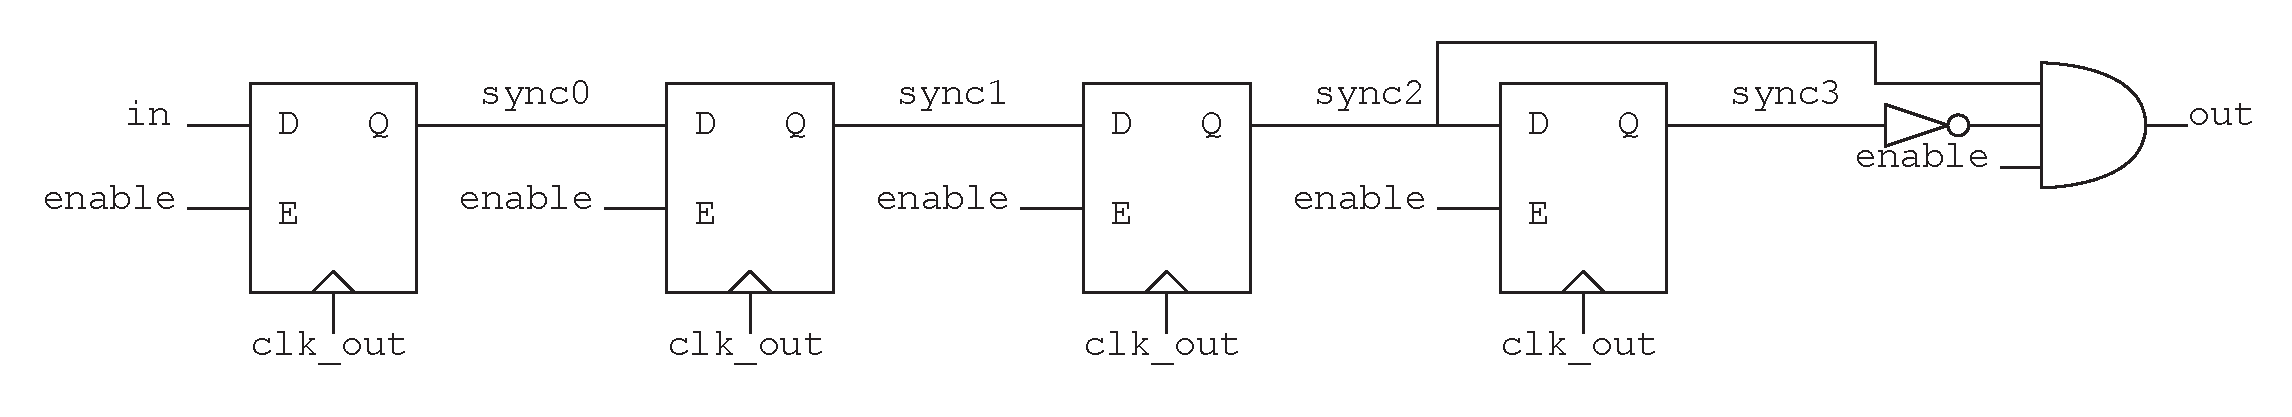
\includegraphics[width=1\linewidth]{bit-sync}
\caption{Schematic of the \texttt{bit\_sync} module}
\label{fig:bit-sync}
\end{figure}

\section{bus\_sync}
\subsection{Description}
This module synchronizes a bus from a slower clock domain to a faster one. In particular, this module behaves somewhat like a FIFO with a depth of 1. The slow clock writes to the \texttt{bus\_sync} module. The written data is copied into another register using the fast clock, and a valid signal is asserted. The faster clock then asserts its read enable signal to indicate that it read the data, and the valid signal is de-asserted.

This module is used in the \texttt{RFcontroller} module to synchronize the length of a packet being received from the \texttt{corr\_despreader} module. The valid signal of this module is used by the \texttt{RFcontroller} both to indicate that the \texttt{corr\_despreader} module has detected an incoming packet, and it has decoded the length of that packet.

\subsection{Input/Output Ports and Parameters}
\begin{description}
	\item[\texttt{reset\_n}] Input reset.
	\item[\texttt{clk}] Input data clock. The input data, \texttt{din}, and the write enable, \texttt{wr\_en}, are aligned to this clock.
	\item[\texttt{sync\_clk}] Input sampling clock. This clock is used to sample the input data. The output data, \texttt{dout}, and the valid output, \texttt{valid}, are aligned to this clock. The write enable input, \texttt{wr\_en}, must also be aligned to this clock.
	\item[\texttt{sync\_en}] Enable input for the entire synchronizer. Both \texttt{wr\_en} and \texttt{rd\_en} are ignored if this input is low. This input must be stable before attempting to write and remain stable as long as this synchronizer is in use.
	\item[\texttt{wr\_en}] Write enable input. This input must be aligned with \texttt{clk}. When this input is high, the input data, \texttt{din} is stored and is eventually written to the data output, \texttt{dout}.
	\item[\texttt{rd\_en}] Read enable input. This input must be aligned with \texttt{sync\_clk}. This input indicates that the data on \texttt{dout} has been read. The \texttt{valid} output de-asserts after a read.
	\item[\texttt{din[BUS\_LENGTH-1:0]}] Input data to be synchronized. This input must be aligned with \texttt{clk}.
	\item[\texttt{dout[BUS\_LENGTH-1:0]}] Synchronized output data. This output is aligned with \texttt{sync\_clk}.
	\item[\texttt{valid}] Data valid output. Indicates that the data on \texttt{dout} is valid. This output is aligned with \texttt{sync\_clk}.
	\item[\texttt{BUS\_LENGTH}] Parameter describing the width of the data buses.
\end{description}

\subsection{Design Details}
This module ignores all inputs as long as the \texttt{sync\_en} input is low. When both \texttt{sync\_en} and \texttt{wr\_en} are asserted, this module samples the data input, \texttt{din}, onto a register using the input clock \texttt{clk}. The \texttt{wr\_en} input itself is also sampled onto a register using \texttt{clk}. The registered version of \texttt{wr\_en} is then sampled into a shift register with a depth 3 using \texttt{sync\_clk}. This shift register is used to reduce the probability of metastability. The last two bits are compared to determine if there is a rising edge. This rising edge indicates that data was previously sampled from \texttt{din}, and that the registered value is currently stable. This rising edge is used to copy the registered \texttt{din} data into another register using \texttt{sync\_clk}. At the same time, the register with the \texttt{valid} output is set. This register is cleared by asserting the \texttt{rd\_en} input. Throughout this entire process the \texttt{sync\_en} input must be high. A schematic of this circuit is shown in Figure \ref{fig:bus-sync}.

This synchronizer design may fail if there are multiple writes in succession, as there is no check to see if the value from a previous write is read before writing again. However, this module is used in a context where multiple writes are not possible. This module is used to only synchronize one signal between two clock domains on a single occasion, and then is reset.

\begin{figure}
\centering
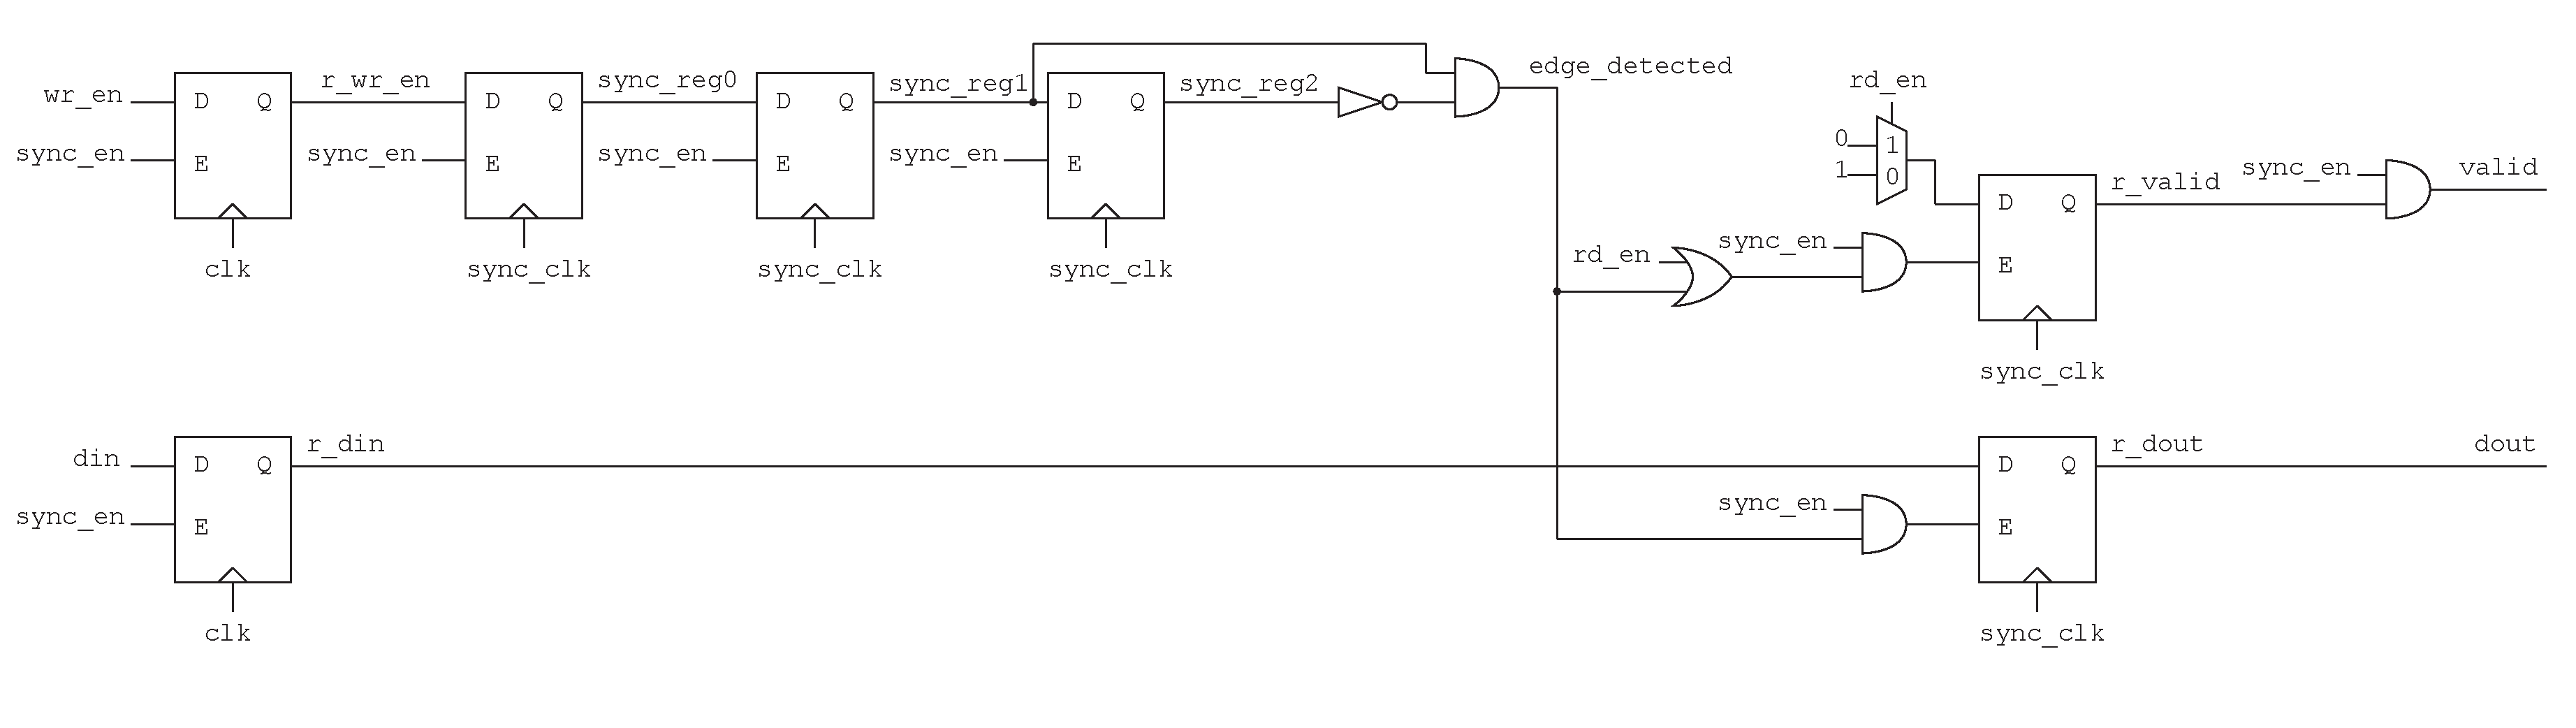
\includegraphics[width=1\linewidth]{bus-sync}
\caption{Schematic of the \texttt{bus\_sync} module}
\label{fig:bus-sync}
\end{figure}

\section{crcParallel}
\subsection{Description}
This module is used by the \texttt{RFcontroller} module to calculate the cyclic redundancy check (CRC) value of a radio packet conforming to the IEEE 802.15.4 standard. This standard uses CRC to detect any errors in a received packet.

The theory behind the CRC calculation may be relatively confusing for those without any experience in error detection and correction; however, its purpose and use is straightforward. The CRC is the result of a mathematical function over the entire payload data of a packet. On the transmission side, a 16-bit CRC is calculated over the payload (up to 127 bytes) and appended to end of the packet. On the receive side, the 16-bit CRC is calculated over the entire payload \textit{and} the additional CRC bits appended to the end of the packet. If the result on the receive end is not 0, then there is an error in the packet payload and the data should be discarded. % the use of should is acceptable here

Typical implementations calculate the CRC input 1 bit of the payload at a time. Such a module requires that the payload data be clocked in serially, from LSB to MSB. However, all of the operations in the \texttt{RFcontroller} module deal with bytes rather than individual bits, and serializing the data for this calculation slows down the overall packet transmission process. Therefore, this implementation was designed to calculate the CRC using inputs of 1 byte instead of 1 bit. The packet data is clocked in 1 byte at a time, from the first byte in the packet (the first byte transmitted) to the last byte in the packet.

For more information on the CRC calculation, see section 5.2.1.9 of the IEEE 802.15.4 standard \cite{15-4-standard}. A copy is found in \path{scm-digital/doc/}.

\subsection{Input/Output Ports}
\begin{description}
	\item[\texttt{HCLK}] Input clock.
	\item[\texttt{HRESETn}] Input reset. This input is used for the main system reset.
	\item[\texttt{local\_rst}] Input reset from the \texttt{RFcontroller}. This input is used when the \texttt{RFcon\-t\-roller} module clears the CRC value between computations. The CRC must be reset before each computation in order to produce the correct result.
	\item[\texttt{sample\_en}] Input indicating that the input is valid and the CRC value must update.
	\item[\texttt{in[7:0]}] Data input. This is the packet payload data.
	\item[\texttt{crc[15:0]}] CRC output. This is the CRC calculated over all of the previous inputs since the module was reset. This value is not valid until the entire packet payload is inputted to this module.
\end{description}

\subsection{Design Details}
Typical CRC implementations use a linear feedback shift register (LFSR) to calculate the CRC 1 bit at a time. This is the method used in section 5.2.1.9 of the IEEE 802.15.4 standard \cite{15-4-standard}.

This module instead calculates the CRC using an 8-bit input by following the method described in \cite{parallel-crc}. The design process involves creating a reference serial implementation (such as an LFSR), and recording the output given a series of particular inputs. These results can be used to determine the output / next state as a function of the 16-bit current state and the 8-bit input.

A testbench was created to compare the results of this module with the serial reference implementation. A large number of random inputs were generated and the outputs were compared for every 16 bits of input. This module matched the serial result in each comparison.

For more information on how to create a parallel CRC calculation using a serial reference, see \cite{parallel-crc}. A copy is found in \path{scm-digital/doc/}.

\section{RFTIMER} \label{rftimer}
\subsection{Description}
This module is a special-purpose timer designed to interface with the \texttt{RFcontroller} module. The timer itself is a counter (with a parameterized width) connected to the \texttt{CLK\_RFTIMER} clock with a frequency of 500kHz. There are 8 compare units (the number of compare units is parameterized) that generate an interrupt to the Cortex-M0 when the counter matches the value stored in the compare unit. The compare units also have the option of sending a trigger to the \texttt{RFcontroller} module. There are also 4 capture units (the number of capture units is parameterized) that capture the value of the timer when it receives either a signal from the Cortex-M0 or an interrupt from the \texttt{RFcontroller} module.

With the correct combination and configuration of compare and capture units, the Single Chip Mote is able to send packets or listen for incoming packets at specific times without any intervention from the software on the Cortex-M0 beyond the initial setup. This module is also suitable as a timer for purposes other than sending or receiving packets.

\subsection{Input/Output Ports and Parameters}
\begin{description}
	\item[\texttt{HRESETn}] Input reset.
	\item[\texttt{HCLK}] System clock input.
	\item[\texttt{TCLK}] Timer clock input.
	\item[\texttt{HSEL}] Slave select input.
	\item[\texttt{HWRITE}] Write select input.
	\item[\texttt{HTRANS[1]}] Transfer type input.
	\item[\texttt{HADDR[31:0]}] Address input.
	\item[\texttt{HWDATA[31:0]}] Write data input.
	\item[\texttt{HRDATA[31:0]}] Read data output.
	\item[\texttt{HREADY}] Transfer finished input. This input indicates that the previous transfer on the bus has finished and that address phase signals must be latched.
	\item[\texttt{HREADYOUT}] Transfer finished output.
	\item[\texttt{tx\_load\_done\_in}] Input from the \texttt{RFcontroller} module to the capture units for the \texttt{TX\_LOAD\_DONE} interrupt.
	\item[\texttt{tx\_sfd\_done\_in}] Input from the \texttt{RFcontroller} module to the capture units for the \texttt{TX\_SFD\_DONE} interrupt.
	\item[\texttt{tx\_send\_done\_in}] Input from the \texttt{RFcontroller} module to the capture units for the \texttt{TX\_SEND\_DONE} interrupt.
	\item[\texttt{rx\_sfd\_done\_in}] Input from the \texttt{RFcontroller} module to the capture units for the \texttt{RX\_SFD\_DONE} interrupt.
	\item[\texttt{rx\_done\_in}] Input from the \texttt{RFcontroller} module to the capture units for the \texttt{RX\_DONE} interrupt.
	\item[\texttt{tx\_load\_trigger\_out}] Output to the \texttt{RFcontroller} module from the compare units for the \texttt{TX\_LOAD} trigger.
	\item[\texttt{tx\_send\_trigger\_out}] Output to the \texttt{RFcontroller} module from the compare units for the \texttt{TX\_SEND} trigger.
	\item[\texttt{rx\_start\_trigger\_out}] Output to the \texttt{RFcontroller} module from the compare units for the \texttt{RX\_START} trigger.
	\item[\texttt{rx\_stop\_trigger\_out}] Output to the \texttt{RFcontroller} module from the compare units for the \texttt{RX\_STOP} trigger.
	\item[\texttt{NUM\_COMPARE\_UNITS}] Parameter describing the number of compare units.
	\item[\texttt{NUM\_CAPTURE\_UNITS}] Parameter describing the number of capture units.
	\item[\texttt{COUNTER\_WIDTH}] Parameter describing the width of the counter used for the timer.
\end{description}

\subsection{Design Details}

\begin{figure}
\centering
\includegraphics[width=1\linewidth, page=2]{rftimer-schematics}
\caption{Register enable signals from the AHB for the \texttt{RFTIMER} module.}
\label{fig:rftimer-wr-en}
\end{figure}

\subsubsection{Clocking Assumptions}
In order for this module to function correctly, the clock frequency of the timer $f_{timer}$ must be a division of the system clock frequency $f_{sys}$ such that $f_{sys} = N \times f_{timer}$, where $N$ is an integer. In the case of the Single Chip Mote digital system on an FPGA, the system clock \texttt{HCLK}, has a frequency of 5MHz, and the timer clock, \texttt{CLK\_RFTIMER} (connected to the \texttt{TCLK} input on this module), has a frequency of 500kHz. The rising edge of the timer clock must be aligned to the rising edge of the system clock. In general this is achieved by having the timer clock and the system clock originate from the same oscillator and using feedback to keep their relative phases in alignment. There are no synchronization issues as long as these requirements are met.

\subsubsection{Synchronization}
The timer operates in the slower timer clock domain, and the AHB bus (that sets the configuration registers) operates in the faster system clock domain. If the relationship between these two clocks is unknown, then the \texttt{RFTIMER} module would require synchronizers to pass data between the two clock domains. However, by requiring that the timer clock and system clock are aligned in phase, the following assumptions are valid:

\begin{itemize}
	\item Registers in the timer clock domain only change their value on the rising edge of the timer clock. Since this coincides with the rising edge of the system clock, the output of those registers are also only changing on the rising edge of the system clock, and are stable at all other times. This means that any logic in the system clock domain can use the output of a register in the timer clock domain without a synchronizer. Therefore, the AHB can directly read any registers in the \texttt{RFTIMER} module that are connected to \texttt{TCLK}.
	\item Logic in the timer clock domain relying on configuration registers in the system clock domain must not be connected directly to the output of those registers. It is possible for registers in the system clock domain to change multiple times during a single timer clock cycle, leading to erratic behavior.
	\item Configuration registers in the system clock domain are safely sampled by registers in the timer clock domain by directly connecting the output of the former to the input of the latter. The data in the configuration register may change many times in a single timer clock cycle, but only the last value is written into the sampling register. The timing tools use the defined phase relationship between the two clock domains to ensure that there are no setup and hold time violations. As a result, the paths between the registers are laid out such that the sampling register does not sample when the input is changing and there is little chance of metastability.
\end{itemize}

Therefore, it is possible to connect signals from between the two clock domains without much overhead. Connecting signals from the system clock domain to the timer clock domain first requires directly sampling the signals in the timer clock domain and then using those sampled outputs in the timer clock domain logic. On the other hand, signals from the timer clock domain are directly connected to logic in the system clock domain. More robust synchronization logic is not necessary.

In the Verilog code for this module, all register names with the \texttt{\_t} suffix indicate that the register is connected to \texttt{TCLK}. All register names with the \texttt{\_h} suffix indicate that the register is connected to \texttt{HCLK}. A common pattern repeated throughout this design is the use of a \texttt{\_h} register written via the AHB and an accompanying \texttt{\_t} register sampling its value on every rising edge of \texttt{TCLK}.

\subsubsection{Counter}
The timer in the \texttt{RFTIMER} module is a counter (with a width of \texttt{COUNTER\_WIDTH}) that increments by 1 on the rising edge of \texttt{TCLK}. The counter value can also be read or written via the \texttt{RFTIMER\_REG\_\_COUNT} register. If at any time the value in this register is greater than or equal to the maximum counter value, stored in the \texttt{RFTIMER\_REG\_\_MAX\_COUNT} register, the counter will roll over back to 0 on the next rising edge of \texttt{TCLK}. This counter is enabled or disabled using the \texttt{ENABLE} bit of the \texttt{RFTIMER\_REG\_\_CONTROL} register, and is reset to 0 using the \texttt{COUNT\_RESET} bit in the same register.

Figure \ref{fig:rftimer-coutner} contains a conceptual schematic and the actual Verilog code for the \texttt{RFTIMER\_REG\_\_COUNT} register (\texttt{count\_t}), the \texttt{RFTIMER\_REG\_\_MAX\_COUNT} register (\texttt{max\_count\_t}), and the \texttt{ENABLE} bit of the \texttt{RFTIMER\_REG\_\_CONTROL} register (\texttt{counter\_en\_t}). The write enable signals are shown in Figure \ref{fig:rftimer-wr-en}. \texttt{max\_count\_t} and \texttt{counter\_en\_t} sample their values from the \texttt{max\_count\_h} and \texttt{counter\_en\_h} registers written by the AHB. The \texttt{count\_t} register samples its value from \texttt{count\_h}.

While the logic at the input to \texttt{count\_h} appears complicated, its function is more straightforward. \texttt{count\_h} always contains the next value of \texttt{count\_t}. The next value of \texttt{count\_t} is either written to a specific value via the AHB, cleared to 0 via the AHB, or set to \texttt{count\_t + 1} when the counter is enabled.

When \texttt{count\_h} is overwritten or cleared via the AHB, \texttt{count\_t} will reflect that change on the next rising edge of \texttt{TCLK}. If there are no AHB writes, \texttt{count\_h} is set to \texttt{count\_t + 1} whenever \texttt{count\_h == count\_t}. When \texttt{count\_t} updates, the condition \texttt{count\_h == cont\_t} is true, and therefore \texttt{count\_h} increments, and again it stores the next value of \texttt{count\_t}. If the timer is disabled (\texttt{counter\_wr\_en == 0}), then \texttt{count\_h} will not update when \texttt{count\_h == count\_t} (although it will update when there is an AHB write since AHB writes must still be take effect when the counter is disabled). There is additional logic to ensure that the value being written to \texttt{count\_h} is not larger than \texttt{max\_count\_t}.

\begin{figure}
	\centering
	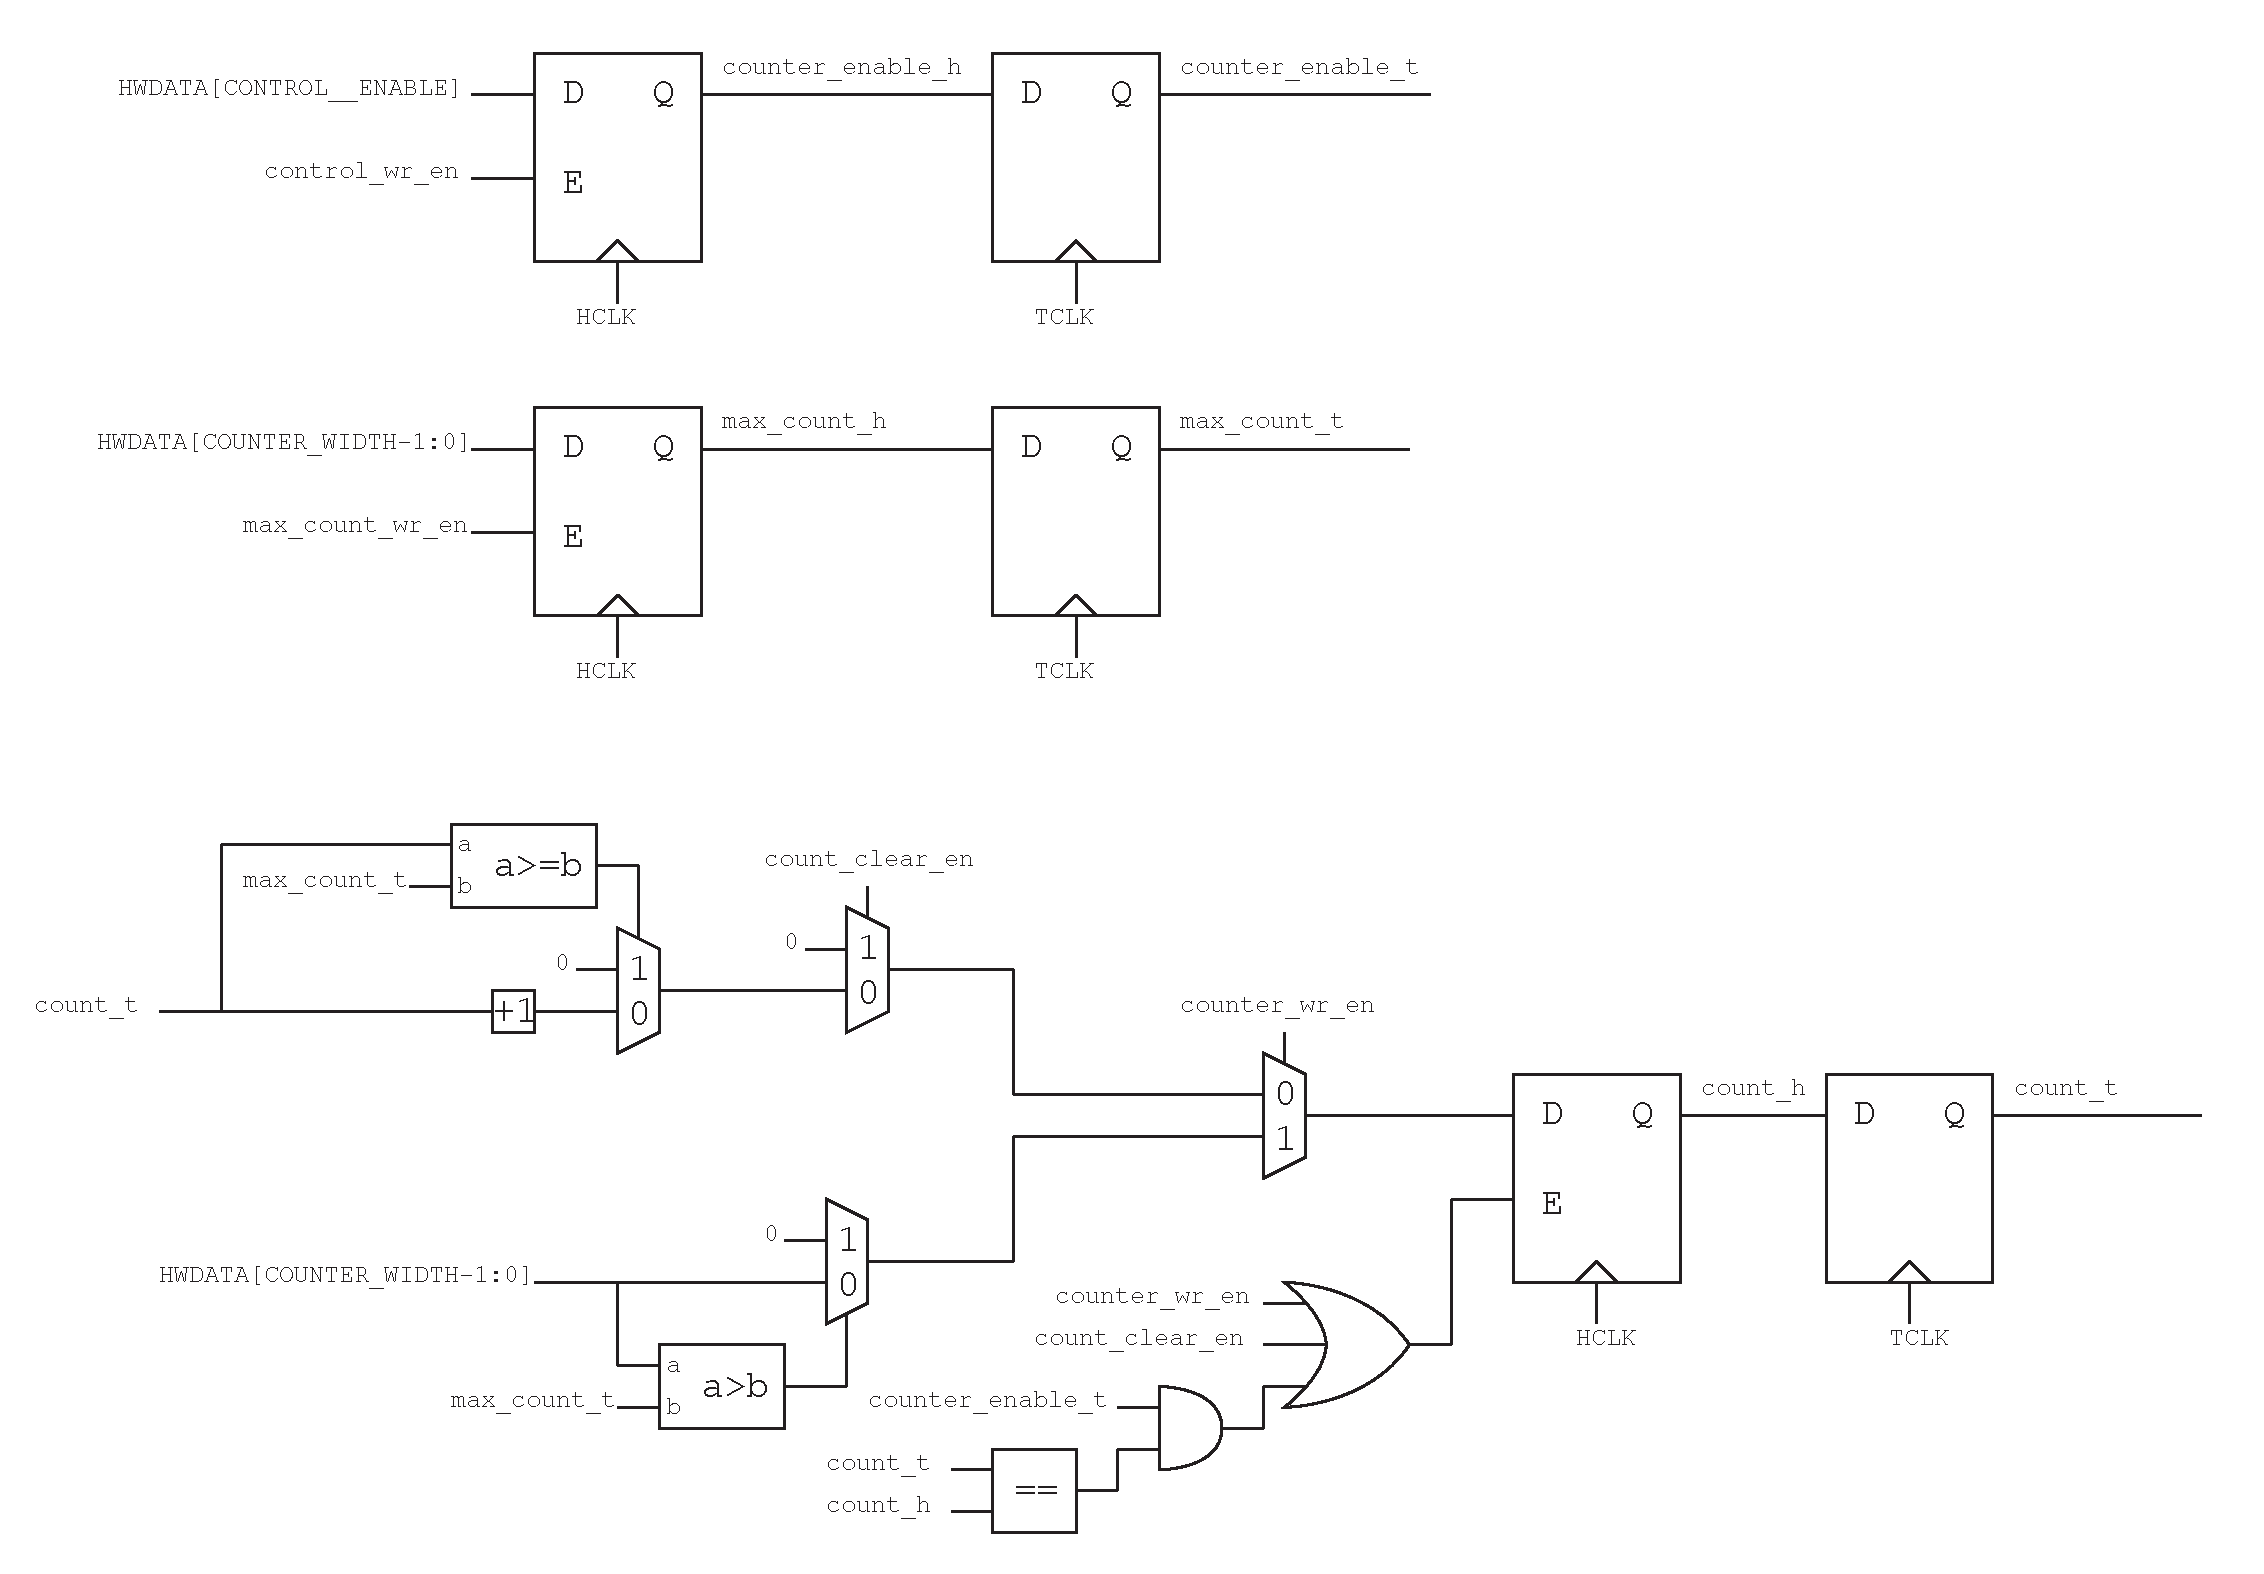
\includegraphics[width=1\linewidth, page=1]{rftimer-schematics}
	\begin{lstlisting}
// Counter Enable Register
always @(posedge HCLK or negedge HRESETn) begin
     if (!HRESETn) counter_enable_h <= 1'b0;
     else if (control_wr_en) counter_enable_h <= HWDATA[CONTROL__ENABLE];
end
always @(posedge TCLK or negedge HRESETn) begin
     if (!HRESETn) counter_enable_t <= 1'b0;
     else counter_enable_t <= counter_enable_h;
end
 
// Max Count Register
always @(posedge HCLK or negedge HRESETn) begin
     if (!HRESETn) max_count_h <= {COUNTER_WIDTH{1'b1}};
     else if (max_count_wr_en) max_count_h <= HWDATA[COUNTER_WIDTH-1:0];
end
always @(posedge TCLK or negedge HRESETn) begin
     if (!HRESETn) max_count_t <= {COUNTER_WIDTH{1'b1}};
     else max_count_t <= max_count_h;
end
 
// Counter
always @(posedge HCLK or negedge HRESETn) begin
   if (!HRESETn) count_h <= 0;
   else if (counter_wr_en)
       if (HWDATA[COUNTER_WIDTH-1:0] > max_count_t) count_h <= 0;
       else count_h <= HWDATA[COUNTER_WIDTH-1:0];
   else if (count_clear_en) count_h <= 0;
   else if ((count_h == count_t) && counter_enable_t)
       if (count_t >= max_count_t) count_h <= 0;
       else count_h <= count_t + 1;
end
always @(posedge TCLK or negedge HRESETn) begin
   if (!HRESETn) count_t <= 0;
   else count_t <= count_h;
end
	\end{lstlisting}
	\caption{Schematic and Verilog code for the \texttt{counter} register, the \texttt{max\_count} register, and the \texttt{counter\_enable} register for the \texttt{RFTIMER} module.}
	\label{fig:rftimer-coutner}
\end{figure}

\subsubsection{Compare Units}
This module has multiple compare units, specified by the \texttt{NUM\_COMPARE\_UNITS} parameter, that store a value to compare against the counter. If the compare value matches the counter, then the compare unit has the option to set a bit in the \texttt{RFTIMER\_REG\_\_INT} register to trigger the Cortex-M0 interrupt, or send a trigger to the \texttt{RFcontroller} module.

Each compare unit has a compare register, \texttt{RFTIMER\_REG\_\_COMPAREi}, and a control register, \texttt{RFTIMER\_REG\_\_COMPAREi\_CONTROL} (where the i represents the index of the compare unit, ranging from 0 to \texttt{NUM\_COMPARE\_UNITS-1}). The compare unit is implemented in the \texttt{compare\_unit} submodule, with connections to the \texttt{RFTIMER} module for the AHB interface and the interrupts.

In order to parameterize the module for different numbers of compare units, each \texttt{compare\_unit} submodule is instantiated inside a generate statement. The following buses and arrays of buses are used to connect to the \texttt{compare\_unit} modules within the generate statement based on their index i:

\begin{description}
	\item[\texttt{comparex\_wr\_en}] Bit i in this bus connects to the write enable signal for the \texttt{RFTIMER\-\_REG\-\_\_COMPAREi} register.
	\item[\texttt{comparex\_control\_wr\_en}] Bit i in this bus connects to the write enable signal for the \texttt{RFTIMER\_REG\_\_COMPAREi\_CONTROL} register.
	\item[\texttt{comparex\_interrupt\_en}] Bit i in this bus connects to the interrupt enable output for compare unit i, used for the Cortex-M0 interrupt.
	\item[\texttt{comparex\_match}] Bit i in this bus connects to the compare match output for compare unit i, used for the Cortex-M0 interrupt.
	\item[\texttt{compare}] Bus i in this array of buses connects to the output of the \texttt{RFTIMER\_REG\-\_\_COMPAREi} register.
	\item[\texttt{compare\_control}] Bus i in this array of buses connects to the output of the \texttt{RFTIMER\-\_REG\-\_\_COMPAREi\_CONTROL} register.
	\item[\texttt{tx\_load\_trigger\_bus}] Bit i in this bus connects to the \texttt{TX\_LOAD} trigger output from compare unit i.
	\item[\texttt{tx\_send\_trigger\_bus}] Bit i in this bus connects to the \texttt{TX\_SEND} trigger output from compare unit i.
	\item[\texttt{rx\_start\_trigger\_bus}] Bit i in this bus connects to the \texttt{TX\_START} trigger output from compare unit i.
	\item[\texttt{rx\_stop\_trigger\_bus}] Bit i in this bus connects to the \texttt{RX\_STOP} trigger output from compare unit i.
\end{description}

For more information on the implementation of the compare units, see section \ref{compare-unit}.

\subsubsection{Capture Units}
This module has multiple capture units, specified by the \texttt{NUM\_CAPTURE\_UNITS} parameter, that store the value of the counter into a register when triggered by the Cortex-M0 via the AHB, or when triggered by an interrupt from the \texttt{RFcontroller} module. This module also has the option to set a bit in the \texttt{RFTIMER\_REG\_\_INT} register to trigger the Cortex-M0 interrupt after a capture.

Each capture unit has a capture register, \texttt{RFTIMER\_REG\_\_CAPTUREi}, and a control register, \texttt{RFTIMER\_REG\_\_CAPTUREi\_CONTROL} (where the i represents the index of the capture unit, ranging from 0 to \texttt{NUM\_CAPTURE\_UNITS-1}). The capture unit is implemented in the \texttt{capture\_unit} submodule, with connections to the \texttt{RFTIMER} module for the AHB interface and the interrupts.

In order to parameterize the module for different numbers of capture units, each \texttt{capture\_unit} submodule is instantiated inside a generate statement. The following buses and arrays of buses are used to connect to the \texttt{capture\_unit} modules within the generate statement based on their index i:

\begin{description}
	\item[\texttt{capturex\_control\_wr\_en}] Bit i in this bus connects to the write enable signal for the \texttt{RFTIMER\_REG\_\_CAPTUREi\_CONTROL} register.
	\item[\texttt{capturex\_interrupt\_en}] Bit i in this bus connects to the interrupt enable output for capture unit i, used for the Cortex-M0 interrupt.
	\item[\texttt{capturex\_trigger}] Bit i in this bus connects to the capture trigger output for capture unit i, used for the Cortex-M0 interrupt.
	\item[\texttt{capture}] Bus i in this array of buses connects to the output of the \texttt{RFTIMER\_REG\-\_\_CAPTUREi} register.
	\item[\texttt{capture\_control}] Bus i in this array of buses connects to the output of the \texttt{RFTIMER\-\_REG\_\_CAPTUREi\_CONTROL} register.
\end{description}

For more information on the implementation of the capture units, see section \ref{capture-unit}.

\subsubsection{Interrupts from the \texttt{RFcontroller} Module}
When configured to do so, the \texttt{RFcontroller} module sends single-cycle (synchronized with \texttt{HCLK}) pulses to the \texttt{RFTIMER} module to trigger a capture on any of the capture units. These pulses come from the \texttt{tx\_load\_done\_in}, \texttt{tx\_sfd\_done\_in}, \texttt{tx\_send\_done\_in}, \texttt{rx\_sfd\_done\_in}, and \texttt{rx\_done\_in} inputs to the \texttt{RFTIMER} module, and are connected directly to each capture unit. The capture units are only triggered when a particular input is enabled in the \texttt{RFTIMER\_REG\_\_CAPTUREi\_CONTROL} register. For more information on the events that trigger these pulses, see section \ref{rfcontroller}.

\subsubsection{Triggers to the \texttt{RFcontroller} Module}
When configured to do so, the \texttt{RFTIMER} module sends single-cycle (synchronized with \texttt{TCLK}) pulses during a compare match to the \texttt{RFcontroller} module. These pulses trigger the state machines controlling the sending and receiving of packets. The compare units only generate a pulse when a particular output is enabled in the \texttt{RFTIMER\_REG\_\_COMPAREi\_CONTROL} register. Each compare unit has four outputs for the four types of triggers: \texttt{tx\_load\_trigger}, \texttt{tx\_send\_trigger}, \texttt{rx\_start\_trigger}, \texttt{rx\_stop\_trigger}. The outputs to the \texttt{RFcontroller} module from the \texttt{RFTIMER} module are the bitwise OR of the outputs from each compare unit.

\subsubsection{Cortex-M0 Interrupt}
This module has one interrupt to the Cortex-M0, through the \texttt{rftimer\_irq} output. This output is the bitwise OR of the bits in the \texttt{RFTIMER\_REG\_\_INT} register, synchronous with \texttt{HCLK}. Each bit in the \texttt{RFTIMER\_REG\_\_INT} corresponds to an interrupt from a compare or capture unit, and is only be set if interrupts are globally enabled by setting the \texttt{INTERRUPT\_ENABLE} bit of the \texttt{RFTIMER\_REG\_\_CONTROL} register. Each bit in this register is cleared by setting the same bit in the \texttt{RFTIMER\_REG\_\_INT\_CLEAR} register.

The \texttt{RFTIMER\_REG\_\_INT} register is a concatenation of three separate registers: \texttt{comaprex\_int}, \texttt{capturex\_int}, and \texttt{capturex\_overflow}. The \texttt{comparex\_int} register has 1 bit for each compare unit, and the \texttt{capturex\_int} and \texttt{capturex\_overflow} registers have 1 bit for each capture unit.

A bit in the \texttt{comparex\_int} register is set when the following conditions are true: there is a compare match, interrupts are globally enabled, and the \texttt{INTERRUPT\_ENABLE} bit of the \texttt{RFTIMER\_REG\_\_COMPAREi\_CONTROL} (assigned to \texttt{comparex\_interrupt\-\_en[i]}) is set. A compare match is indicated by the \texttt{comparex\_match[i]} signal, a single-cycle pulse synchronous with \texttt{TCLK}. In order to prevent this pulse from writing to the interrupt register multiple times (since the \texttt{comparex\_int} register is synchronous with \texttt{HCLK}), an edge detection circuit is used to sample the \texttt{comparex\_match[i]} signal and set \texttt{comparex\_int[i]} on the rising edge. A conceptual schematic of this edge detection circuit and the \texttt{comparex\_int[i]} register is shown in Figure \ref{fig:compare-int} along with the actual Verilog code. The two \texttt{edge\_detect} registers are designed to clear themselves if the interrupt is disabled.

A bit in the \texttt{capturex\_int} register is set when the following conditions are true: a capture is triggered, interrupts are globally enabled, and the \texttt{INTERRUPT\_ENABLE} bit of the \texttt{RFTIMER\_REG\_\_CAPTUREi\_CONTROL} (assigned to \texttt{capturex\_interrupt\_en[i]}) is set. A capture trigger is indicated by the \texttt{capturex\_trigger[i]} signal, a single-cycle pulse synchronous with \texttt{HCLK}. If the \texttt{capturex\_int[i]} bit is not cleared before the next capture event, the corresponding bit in the \texttt{capturex\_overflow} register is set instead.  A conceptual schematic of the \texttt{capturex\_int[i]} and \texttt{capturex\_over\-flow[i]} registers is shown in Figure \ref{fig:capture-int}, along with the actual Verilog code.

\begin{figure}
	\centering
	\includegraphics[width=1\linewidth, page=5]{rftimer-schematics}
	\begin{lstlisting}
// Compare Interrupts
generate
for (i = 0; i < NUM_COMPARE_UNITS; i = i + 1) begin : compare_interrupts
    always @(posedge HCLK or negedge HRESETn) begin
        if (!HRESETn) edge_detect0[i] <= 1'b0;
        else if (global_int_enable_t && comparex_interrupt_en[i]) edge_detect0[i] <= comparex_match[i];
        else if (edge_detect0[i]) edge_detect0[i] <= 1'b0;
    end
    always @(posedge HCLK or negedge HRESETn) begin
        if (!HRESETn) edge_detect1[i] <= 1'b0;
        else if (global_int_enable_t && comparex_interrupt_en[i]) edge_detect1[i] <= edge_detect0[i];
        else if (edge_detect1[i]) edge_detect1[i] <= 1'b0;
    end
    always @(posedge HCLK or negedge HRESETn) begin
        if (!HRESETn) comparex_int[i] <= 1'b0;
        else if (global_int_enable_t && edge_detect0[i] && !edge_detect1[i]) comparex_int[i] <= 1'b1;
        else if (int_clear_wr_en && HWDATA[i]) comparex_int[i] <= 1'b0;
    end
end
endgenerate
	\end{lstlisting}
	\caption{Schematic and Verilog code for the \texttt{comparex\_int[i]} register for the \texttt{RFTIMER} module.}
	\label{fig:compare-int}
\end{figure}
\begin{figure}
	\centering
	\includegraphics[width=1\linewidth, page=6]{rftimer-schematics}
	\begin{lstlisting}
// Capture Interrupts
generate
for (i = 0; i < NUM_CAPTURE_UNITS; i = i + 1) begin : capture_interrupts
    always @(posedge HCLK or negedge HRESETn) begin
        if (!HRESETn) capturex_int[i] <= 1'b0;
        else if (global_int_enable_t && capturex_trigger[i] && capturex_interrupt_en[i] && !capturex_int[i]) capturex_int[i] <= 1'b1;
        else if (int_clear_wr_en && HWDATA[NUM_COMPARE_UNITS+i]) capturex_int[i] <= 1'b0;
    end
    always @(posedge HCLK or negedge HRESETn) begin
        if (!HRESETn) capturex_overflow[i] <= 1'b0;
        else if (global_int_enable_t && capturex_trigger[i] && capturex_interrupt_en[i] && capturex_int[i]) capturex_overflow[i] <= 1'b1;
        else if (int_clear_wr_en && HWDATA[NUM_COMPARE_UNITS+NUM_CAPTURE_UNITS+i]) capturex_overflow[i] <= 1'b0;
    end
end
endgenerate
	\end{lstlisting}
	\caption{Schematic and Verilog code for the \texttt{capturex\_int[i]} and \texttt{capturex\_overflow[i]} registers for the \texttt{RFTIMER} module.}
	\label{fig:capture-int}
\end{figure}

\subsection{Register Interface} \label{rftimer-registers}
\subsubsection{Control Register}
The counter is controlled using the \texttt{RFTIMER\_REG\_\_CONTROL} register. This register has three bits, \texttt{ENABLE}, \texttt{INTERRUPT\_ENABLE}, and \texttt{COUNT\_RESET}. Setting the \texttt{ENABLE} bit of this register causes the counter to increment during each timer clock cycle that the \texttt{ENABLE} bit is set to 1. The counter does not increment if the \texttt{ENABLE} bit is set to 0, and continues to increment from the current value of \texttt{RFTIMER\_REG\_\_COUNT} when re-enabled. The \texttt{INTERRUPT\_ENABLE} bit is a global enable signal for all of the compare/capture interrupts. Setting the \texttt{COUNT\_RESET} bit resets the value of the counter back to 0 on the next timer clock (\texttt{TCLK}) cycle. While it is also possible to reset the timer by writing a 0 to the \texttt{RFTIMER\_REG\_\_COUNT} register, the \texttt{COUNT\_RESET} bit allows the software to reset and enable the timer in a single register write access. If multiple changes are made to the \texttt{RFTIMER\_REG\_\_CONTROL} register during a single timer clock (\texttt{TCLK}) cycle, only the last change takes effect on the next rising edge of the timer clock.

\subsubsection{Counter and Max Count Registers}
The counter value is stored on the \texttt{RFTIMER\_REG\_\_COUNTER} register, with a width equal to the \texttt{COUNTER\_WIDTH} parameter. The \texttt{RFTIMER\_REG\_\_MAX\_COUNT} register contains the maximum value of the counter before it rolls over to 0. When the timer is enabled, the counter value increments by 1 with each rising edge of the timer clock (\texttt{TCLK}). The \texttt{RFTIMER\_REG\_\_COUNTER} register can also be written by the software, including when the timer is enabled. When the counter reaches the value in the \texttt{RFTIMER\_REG\_\_MAX\_COUNT} register, it rolls over back to 0 on the next rising edge. If \texttt{RFTIMER\_REG\_\_MAX\_COUNT} is changed when the counter value is greater than or equal to the new \texttt{RFTIMER\_REG\_\_MAX\_COUNT} value, then the counter rolls over to 0 on the next rising edge. If multiple changes are made to the \texttt{RFTIMER\_REG\_\_COUNTER} and \texttt{RFTIMER\_REG\_\_MAX\_COUNT} registers during a single timer clock (\texttt{TCLK}) cycle, only the last change takes effect on the next rising edge of the timer clock.

\subsubsection{Compare Unit i Registers}
The \texttt{RFTIMER\_REG\_\_COMPAREi} register, with width equal to the \texttt{COUNTER\_WIDTH} parameter, contains the value that is compared to the counter in compare unit i. Each compare unit, when configured to do so, generates an interrupt to the Cortex-M0 on the next rising edge of the system clock (\texttt{HCLK}) after the counter value matches the value stored in the \texttt{RFTIMER\_REG\_\_COMPAREi} register. Each compare unit also has the option of sending a trigger to the \texttt{RFcontroller} module with a single-cycle pulse (according to \texttt{TCLK}) when the counter matches the value stored in the \texttt{RFTIMER\_REG\_\_COMPAREi} register.

The \texttt{RFTIMER\_REG\_\_COMPAREi\_CONTROL} register contains six bits to enable the compare unit and configure its interrupts and triggers. The \texttt{ENABLE} bit must be set in order for the compare unit to generate an interrupt or trigger. The other five bits enable or disable the individual interrupts and triggers.

The compare unit is capable of generating five different types of interrupts or triggers in any combination. The first is an interrupt to the Cortex-M0, enabled by setting the \texttt{INTERRUPT\_ENABLE} bit of the \texttt{RFTIMER\_REG\_\_COMPAREi\_CONTROL} register. This interrupt causes the corresponding bit in the \texttt{RFTIMER\_REG\_\_INT} register to be set. The other four are triggers for the \texttt{RFcontroller} module. These triggers are enabled by setting the \texttt{TX\_LOAD\_ENABLE}, \texttt{TX\_SEND\_ENABLE}, \texttt{RX\_START\_ENABLE} and \texttt{RX\_STOP\_ENABLE} bits in the \texttt{RFTIMER\_REG\_\_COMPAREi\_CONTROL} register. These triggers activate the state machines in the \texttt{RFcontroller} module to load the TX FIFO with the packet data, send the data in the TX FIFO, turn on the radio to listen for packets, and turn off the radio after listening for packets, respectively. The four triggers are intended to be mutually exclusive, though this is not enforced in the compare unit logic. For more information on these triggers and how they interact with the \texttt{RFcontroller} module, see  section \ref{rfcontroller}.

Changes can be made to both the \texttt{RFTIMER\_REG\_\_COMPAREi} and \texttt{RFTIMER\_REG\-\_\_COMPAREi\_CONTROL} registers when the counter is enabled. If multiple changes are made during a single timer clock cycle, only the last change takes effect on the next rising edge of the timer clock.

\subsubsection{Capture Unit i Registers}
The \texttt{RFTIMER\_REG\_\_CAPTUREi} register, with width equal to the \texttt{COUNTER\_WIDTH} parameter, stores the value of the counter register when  of the enabled inputs to the capture unit is asserted. The write is enabled on the next rising edge of the system clock (\texttt{HCLK}) after the input is asserted, and therefore the input must be asserted for at least 1 \texttt{HCLK} cycle.

The \texttt{RFTIMER\_REG\_\_CAPTUREi\_CONTROL} register contains nine bits to configure the inputs and interrupts to the capture unit. If the \texttt{INTERRUPT\_ENABLE} bit is set, a capture event triggers an interrupt to the Cortex-M0, by setting the corresponding bit in the \texttt{RFTIMER\_REG\_\_INT} register on the next rising edge of the system clock (\texttt{HCLK}). If the \texttt{INTERRUPT\_ENABLE} bit is set and the corresponding bit in \texttt{RFTIMER\_REG\_\_INT} register is not cleared before the next trigger/capture event, the corresponding overflow bit is also set in the \texttt{RFTIMER\_REG\_\_INT} register. If there is an overflow then the value in the \texttt{RFTIMER\_REG\_\_CAPTUREi} register is overwritten. If the \texttt{INTERRUPT\_ENABLE} is not set, then the value in the \texttt{RFTIMER\_REG\_\_CAPTUREi} register is overwritten, and there is no indication to the Cortex-M0 of a capture event or an overflow.

There are six possible inputs for triggering each capture unit. These inputs can be enabled by setting the \texttt{INPUT\_SEL\_SOFTWARE}, \texttt{INPUT\_SEL\_TX\_LOAD\_DONE}, \texttt{INPUT\_SEL\_TX\_SFD\_DONE}, \texttt{INPUT\_SEL\_TX\_SEND\_DONE}, \texttt{INPUT\_SEL\_RX\_SFD\_DONE}, and \texttt{INPUT\_SEL\_RX\_DONE} bits in the \texttt{RFTIMER\_REG\_\_CAPTUREi\_CONTROL} register. The first input is from the Cortex-M0, and is triggered when the software sets the \texttt{CAPTURE\_NOW} bit of the \texttt{RFTIMER\_REG\_\_CAPTUREi\_CONTROL} register. The other five inputs are from the \texttt{RFcontroller} module. These inputs are single-cycle (using the system clock \texttt{HCLK}) pulses that indicate when loading the TX FIFO from data memory is done, transmitting the SFD of a packet is done, transmitting an entire packet is done, the SFD of a packet has been received, and an entire packet has been received and stored in data memory, respectively. For more information on these inputs from the \texttt{RFcontroller} module and their significance, see section \ref{rfcontroller}.

Setting the \texttt{CLEAR} bit of the \texttt{RFTIMER\_REG\_\_CAPTUREi\_CONTROL} register resets the value in the \texttt{RFTIMER\_REG\_\_CAPTUREi} register back to 0 on the next rising edge of the system clock (\texttt{HCLK}). If the software sets the \texttt{CLEAR} bit during the same system clock (\texttt{HCLK}) cycle that one of the inputs is triggered, then the trigger overrides the clear, and the value of the counter is copied into the \texttt{RFTIMER\_REG\_\_CAPTUREi} register.

Changes can be made to the \texttt{RFTIMER\_REG\_\_CAPTUREi\_CONTROL} register when the counter is enabled. If multiple changes are made during a single timer clock cycle, only the last change takes effect on the next rising edge of the timer clock.

\subsubsection{Interrupt and Interrupt Clear Registers}
The \texttt{RFTIMER} module has one interrupt to the Cortex-M0. This interrupt is the bitwise OR of all of the bits in the \texttt{RFTIMER\_REG\_\_INT} register, where each bit corresponds to one interrupt source in the \texttt{RFTIMER} module. This interrupt is also globally enabled or disabled using the \texttt{INTERRUPT\_ENABLE} bit of the \texttt{RFTIMER\_REG\_\_CONTROL} register.

The \texttt{RFTIMER\_REG\_\_INT} register contains 16 bits, eight of them corresponding to the interrupts of the compare units, four of them corresponding to the interrupts of the capture units, and four of them corresponding to the overflow bits of the capture units. Each bit in \texttt{RFTIMER\_REG\_\_INT} is set automatically by the \texttt{RFTIMER} module in the event of an interrupt from its corresponding capture/compare unit. Each bit in the \texttt{RFTIMER\_REG\_\_INT} is cleared by setting the corresponding bit in the \texttt{RFTIMER\_REG\_\_INT\_CLEAR} register.

If the interrupt service routine does not disable the counter after an interrupt, then the timer may generate other interrupts as the service routine is running. If there are bits in \texttt{RFTIMER\_REG\_\_INT} that are not cleared before the interrupt service routine returns, then the interrupt signal will remain high, and the Cortex-M0 will execute the interrupt service routine again until all bits in \texttt{RFTIMER\_REG\_\_INT} are cleared.

It is recommended that the interrupt service routine store the value of \texttt{RFTIMER\-\_REG\_\_INT}, perform any necessary actions, and then write that stored value to \texttt{RFTIMER\_REG\_\_INT}. This ensures that any additional interrupts as the service routine is running are not accidentally cleared, and the interrupt service routine is called again to handle with the new interrupts.

\subsubsection{Register Descriptions}
\ExecuteMetaData[chapters/registers.tex]{rftimer-registers}

\section{compare\_unit} \label{compare-unit}
\subsection{Description}
This module is part of the \texttt{RFTIMER} module, and implements the functionality for one of its compare units. This module stores a compare value and generates interrupts when the value of the counter from the \texttt{RFTIMER} module matches the compare value. One of the interrupts is for the Cortex-M0, and the other four are triggers for the state machines inside the \texttt{RFcontroller} module. The interrupt and trigger outputs from this module are synchronous with the timer clock (\texttt{TCLK}). For more details on the purpose and function of this module within the \texttt{RFTIMER} design, see section \ref{rftimer}.

\subsection{Input/Output Ports and Parameters}
\begin{description}
	\item[\texttt{HRESETn}] Input reset.
	\item[\texttt{HCLK}] System clock input.
	\item[\texttt{TCLK}] Timer clock input.
	\item[\texttt{HWDATA[COUNTER\_WIDTH-1:0]}] Write data input. Used for AHB writes to the compare and compare control registers.
	\item[\texttt{count[COUNTER\_WIDTH-1:0]}] Counter input from the \texttt{RFTIMER} module.
	\item[\texttt{compare\_wr\_en}] Write enable input for the compare register.
	\item[\texttt{compare\_control\_wr\_en}] Write enable input for the compare control register.
	\item[\texttt{tx\_load\_trigger}] Output to the \texttt{RFcontroller} module for the \texttt{TX\_LOAD} trigger.
	\item[\texttt{tx\_send\_trigger}] Output to the \texttt{RFcontroller} module for the \texttt{TX\_SEND} trigger.
	\item[\texttt{rx\_start\_trigger}] Output to the \texttt{RFcontroller} module for the \texttt{RX\_START} trigger.
	\item[\texttt{rx\_stop\_trigger}] Output to the \texttt{RFcontroller} module for the \texttt{RX\_STOP} trigger.
	\item[\texttt{compare[COUNTER\_WIDTH-1:0]}] Compare register output. Used for AHB reads from the compare register.
	\item[\texttt{compare\_control[5:0]}] Compare control register output. Used for AHB reads from the compare control register.
	\item[\texttt{compare\_match}] Compare match output. Used for the interrupt to the Cortex-M0.
	\item[\texttt{interrupt\_en}] Interrupt enable output from the compare control register. Used for the interrupt to the Cortex-M0.
	\item[\texttt{COUNTER\_WIDTH}] Parameter describing the width of the counter used for the timer.
\end{description}

\subsection{Design Details}
As with the \texttt{RFTIMER} module, all register names with the \texttt{\_t} suffix indicate that the register is connected to \texttt{TCLK}. All register names with the \texttt{\_h} suffix indicate that the register is connected to \texttt{HCLK}. A common pattern repeated throughout this design is the use of a \texttt{\_h} register written via the AHB and an accompanying \texttt{\_t} register sampling its value on every rising edge of \texttt{TCLK}.

This module has a pair of \texttt{\_t} and \texttt{\_h} registers for each bit in the compare control register: \texttt{ENABLE}, \texttt{INTERRUPT\_ENABLE}, \texttt{TX\_LOAD\_ENABLE}, \texttt{TX\_SEND\_ENABLE}, \texttt{RX\_START\_ENABLE}, and \texttt{RX\_STOP\_ENABLE}. The \texttt{\_t} registers for the compare control register are concatenated together to make the \texttt{compare\_control} output. The \texttt{compare\_t}/\texttt{compare\_h} pair stores the compare register value, and \texttt{compare\_t} is connected to the \texttt{compare} output.

The \texttt{compare\_match} output is set to \texttt{count == compare\_t} as long as the \texttt{compare\-\_enable\_t} register is high. Otherwise, the output stays low. Since both \texttt{count} and \texttt{compare\_t} are synchronous with \texttt{TCLK}, the \texttt{compare\_match} output is also synchronous with \texttt{TCLK}.

Each trigger output is the bitwise AND of the trigger's enable register and \texttt{compare\_match}. The enable registers and \texttt{compare\_match} are synchronous with \texttt{TCLK}, and therefore the trigger outputs are also synchronous with \texttt{TCLK}.

A schematic of the compare register, compare control registers, and trigger outputs is shown in Figure \ref{fig:compare-unit}.

\begin{figure}
	\centering
	\includegraphics[width=1\linewidth, page=3]{rftimer-schematics}
	\caption{Schematic for the \texttt{compare\_unit} module.}
	\label{fig:compare-unit}
\end{figure}

\section{capture\_unit} \label{capture-unit}
\subsection{Description}
This module is part of the \texttt{RFTIMER} module, and implements the functionality for one of its capture units. This module monitors several interrupts, and stores the value of the counter from the \texttt{RFTIMER} module when one of those interrupts is asserted. One of these interrupts comes from the Cortex-M0 via the AHB, and the other five come from the \texttt{RFcontroller} module. For more details on the purpose and function of this module within the \texttt{RFTIMER} design, see section \ref{rftimer}.

\subsection{Input/Output Ports and Parameters}
\begin{description}
	\item[\texttt{HRESETn}] Input reset.
	\item[\texttt{HCLK}] System clock input.
	\item[\texttt{TCLK}] Timer clock input.
	\item[\texttt{HWDATA[8:0]}] Write data input. Used for AHB writes to the capture control register.
	\item[\texttt{count[COUNTER\_WIDTH-1:0]}] Counter input from the \texttt{RFTIMER} module.
	\item[\texttt{capture\_control\_wr\_en}] Write enable input for the capture control register.
	\item[\texttt{tx\_load\_done\_in}] Input from the \texttt{RFcontroller} module for the \texttt{TX\_LOAD\_DONE} interrupt.
	\item[\texttt{tx\_sfd\_done\_in}] Input from the \texttt{RFcontroller} module for the \texttt{TX\_SFD\_DONE} interrupt.
	\item[\texttt{tx\_send\_done\_in}] Input from the \texttt{RFcontroller} module for the \texttt{TX\_SEND\_DONE} interrupt.
	\item[\texttt{rx\_sfd\_done\_in}] Input from the \texttt{RFcontroller} module for the \texttt{RX\_SFD\_DONE} interrupt.
	\item[\texttt{rx\_done\_in}] Input from the \texttt{RFcontroller} module for the \texttt{RX\_DONE} interrupt.
	\item[\texttt{capture\_trigger}] Capture trigger output. Used for the interrupt to the Cortex-M0.
	\item[\texttt{capture[COUNTER\_WIDTH-1:0]}] Capture register output. Used for AHB reads from the capture register.
	\item[\texttt{capture\_control[6:0]}] Capture control register output. Used for AHB reads from the capture control register.
	\item[\texttt{interrupt\_en}] Interrupt enable output from the capture control register. Used for the interrupt to the Cortex-M0.
	\item[\texttt{COUNTER\_WIDTH}] Parameter describing the width of the counter used for the timer.
\end{description}

\subsection{Design Details}
As with the \texttt{RFTIMER} module, all register names with the \texttt{\_t} suffix indicate that the register is connected to \texttt{TCLK}. All register names with the \texttt{\_h} suffix indicate that the register is connected to \texttt{HCLK}. A common pattern repeated throughout this design is the use of a \texttt{\_h} register written via the AHB and an accompanying \texttt{\_t} register sampling its value on every rising edge of \texttt{TCLK}.

This module has a pair of \texttt{\_t} and \texttt{\_h} registers for each read-write bit in the capture control register: \texttt{INTERRUPT\_ENABLE}, \texttt{INPUT\_SEL\_SOFTWARE}, \texttt{INPUT\_SEL\_TX\-\_LOAD\_DONE}, \texttt{INPUT\_SEL\_TX\_SFD\_DONE}, \texttt{INPUT\_SEL\_TX\_SEND\_DONE},
\texttt{INPUT\_SEL\_RX\-\_SFD\_DONE}, and \texttt{INPUT\_SEL\_RX\_DONE}. The \texttt{\_t} registers for the capture control register are concatenated together to make the \texttt{capture\_control} output. The \texttt{CAPTURE\-\_NOW} and \texttt{CLEAR} bits are write enable signals for the capture register, and are not part of the \texttt{capture\_control} output, as they are write-only bits in the register.

The \texttt{capture\_trigger} signal is the bitwise OR of all the possible capture interrupts after their bitwise AND with the corresponding input select signals. The \texttt{capture\_h} register is updated with the \texttt{count} register value when \texttt{capture\_trigger} is high on the rising edge of \texttt{HCLK}. The \texttt{capture\_h} register is also cleared when the \texttt{CLEAR} bit of the control register is written and \texttt{capture\_clear\_en} is high. If both \texttt{capture\_trigger} and \texttt{capture\_clear\_en} are asserted, the trigger takes precedence and the \texttt{count} value is copied into \texttt{capture\_h}.

The capture register, \texttt{capture\_h}, uses a synchronous enable to store the counter value. The synchronous enable imposes the requirement that the interrupt input is high for at least 1 clock cycle. The capture register is attached to the system clock (\texttt{HCLK}) and all input pulses must be asserted for at least 1 system clock cycle. An asynchronous alternative is to attach the interrupt inputs directly to the clock input of the \texttt{capture\_h} register. However, this method carries the risk of capturing the counter as the value is changing, leading to metastability. This method is also not recommended on FPGAs as it requires connecting several non-clock signals to dedicated clock nets. Given the intended use of this module, to capture only when directed by the Cortex-M0 or through the \texttt{RFcontroller} module, both synchronous with the system clock, the former method is acceptable.

A schematic of the capture register and capture control registers is shown in Figure \ref{fig:capture-unit}.

\begin{figure}
	\centering
	\includegraphics[width=1\linewidth, page=4]{rftimer-schematics}
	\caption{Schematic for the \texttt{capture\_unit} module.}
	\label{fig:capture-unit}
\end{figure}

\section{AHB2APB}
\subsection{Description}
This module is designed by Bigazzi to act as a bridge connecting the AHB and the APB buses. This module is the master of the APB bus, and creates all of the APB master signals sent to the \texttt{APBMUX} and all APB slaves.

\subsection{Input/Output Ports}
\begin{description}
	\item[\texttt{HCLK}] Input clock. Used on both AHB and APB interfaces.
	\item[\texttt{HRESETn}] Input reset. Used on both AHB and APB interfaces.
	\item[\texttt{HADDR[31:16]}] AHB input address. Since the APB is a 16-bit bus, only the 16 upper bits of \texttt{HADDR} are needed. The rest are omitted.
	\item[\texttt{HTRANS[1]}] AHB transfer type input.
	\item[\texttt{HWRITE}] AHB write select input.
	\item[\texttt{HWDATA[15:0]}] AHB write data input. Since the APB is a 16-bit bus, only the 16 lower bits of \texttt{HWDATA} used. The rest are omitted.
	\item[\texttt{HSEL}] AHB slave select input.
	\item[\texttt{HREADY}] AHB transfer finished input. This input indicates that the previous transfer on the bus has finished and that address phase signals must be latched.
	\item[\texttt{HRDATA[31:0]}] AHB read data output.
	\item[\texttt{HREADYOUT}] AHB transfer finished output.
	\item[\texttt{PADDR[15:0]}] APB address output.
	\item[\texttt{PENABLE}] APB access phase enable output.
	\item[\texttt{PWRITE}] APB write select output.
	\item[\texttt{PWDATA[15:0]}] APB write data output.
	\item[\texttt{PRDATA[15:0]}] APB read data input.
	\item[\texttt{PREADY}] APB transfer finished input.
\end{description}

\subsection{Design Details}
This module operates in three states, \texttt{ST\_IDLE}, \texttt{ST\_SETUP}, \texttt{ST\_ACCESS}. During the \texttt{ST\_IDLE} state, the bridge waits for an AHB transfer addressing one of the APB peripherals. Once a transfer is detected, the bridge latches the AHB address phase signals, and changes to the \texttt{ST\_SETUP} state. This state corresponds to the setup phase of the APB transfer. Meanwhile, the AHB master is stalled by setting \texttt{HREADYOUT} to 0. After the \texttt{ST\_SETUP} state is the \texttt{ST\_ACCESS} state, corresponding to the access phase of the APB transfer. The bridge stays in this state until the slave indicates the state is complete using \texttt{PREADY}. All of the APB slave signals are also routed to the AHB master, as the APB access phase is the same as the AHB data phase. Once the transfer is complete, the bridge transitions to the \texttt{ST\_SETUP} phase if there is another AHB transfer, or transitions to the \texttt{ST\_IDLE} state if there are no more AHB transfers.

\section{APBMUX}
\subsection{Description}
This module is designed by Bigazzi to determine which APB slave is being accessed and route the correct set of slave signals to the APB master. It also decodes \texttt{HADDR[31:24]} to generate a \texttt{PSEL} signal for each slave. This module currently supports four APB slaves; however, with modifications this module may support any number of APB slaves.

\subsection{Input/Output Ports}
\begin{description}
	\item[\texttt{PADDR[15:8]}] Address input. Only the 8 upper bits are necessary and the other bits are omitted.
	\item[\texttt{PRDATA0[15:0]}] Read data input from the first APB slave. In the Single Chip Mote digital system this is the \texttt{APBADC\_V2} module.
	\item[\texttt{PREADY0}] Transfer finished input from the first APB slave. In the Single Chip Mote digital system this is the \texttt{APBADC\_V2} module.
	\item[\texttt{PRDATA1[15:0]}] Read data input from the second APB slave. In the Single Chip Mote digital system this is the \texttt{APBUART} module.
	\item[\texttt{PREADY1}] Transfer finished input from the second APB slave. In the Single Chip Mote digital system this is the \texttt{APBUART} module.
	\item[\texttt{PRDATA2[15:0]}] Read data input from the third APB slave. In the Single Chip Mote digital system this is the \texttt{APB\_ANALOG\_CFG} module.
	\item[\texttt{PREADY2}] Transfer finished input from the third APB slave. In the Single Chip Mote digital system this is the \texttt{APB\_ANALOG\_CFG} module.
	\item[\texttt{PRDATA3[15:0]}] Read data input from the fourth APB slave. In the Single Chip Mote digital system this is the \texttt{APBGPIO} module.
	\item[\texttt{PREADY3}] Transfer finished input from the fourth APB slave. In the Single Chip Mote digital system this is the \texttt{APBGPIO} module.
	\item[\texttt{PRDATA[15:0]}] Read data output to the APB master.
	\item[\texttt{PREADY}] Transfer finished output to the APB master.
	\item[\texttt{PSEL0}] Slave select output for the first APB slave. In the Single Chip Mote digital system this is the \texttt{APBADC\_V2} module.
	\item[\texttt{PSEL1}] Slave select output for the second APB slave. In the Single Chip Mote digital system this is the \texttt{APBUART} module.
	\item[\texttt{PSEL2}] Slave select output for the third APB slave. In the Single Chip Mote digital system this is the \texttt{APB\_ANALOG\_CFG} module.
	\item[\texttt{PSEL3}] Slave select output for the fourth APB slave. In the Single Chip Mote digital system this is the \texttt{APBGPIO} module.
\end{description}

\subsection{Design Details}
This module only contains combinational logic to set the \texttt{PSEL} outputs and choose the correct slave inputs for \texttt{PRDATA} and \texttt{PREADY} using the 8 upper bits of \texttt{HADDR}. This is done using a case statement with the prefixes defined in \texttt{REGISTERS.vh}.

\subsection{Adding Another APB Slave}
Adding a new APB slave in this module requires the following steps:

\begin{enumerate}
	\item Define an address prefix for the slave in \texttt{REGISTERS.vh}.
	\item Add another \texttt{PSEL} output.
	\item Add another \texttt{PRDATA} input.
	\item Add another \texttt{PREADY} input
	\item Add another case to the case statement using the new address prefix. Assign the new \texttt{PSEL} output. Assign \texttt{PRDATA} and \texttt{PREADY}.
	\item Connect the new \texttt{PSEL} output to the new slave/peripheral in the top module, \texttt{uCONTROLLER}.
	\item Connect the new \texttt{PRDATA} and \texttt{PREADY} inputs to the new slave/peripheral in the top module, \texttt{uCONTROLLER}.
\end{enumerate}

\section{APBUART}
\subsection{Description}
This module is a slightly modified version of the \texttt{AHBUART} module provided in the DesignStart kit. Bigazzi adapted the original code to be used on the APB bus instead of the AHB, and parameterized the section of the code used to send data at the appropriate baud rate.

The \texttt{APBUART} module implements a 3-wire serial interface. The data is transmitted in individual data frames containing one start bit, 8 data bits, 1 stop bit, and no extra parity bits. This module also does not implement any flow control. The baud rate is determined based on the \texttt{UARTBAUDGEN} parameter in \texttt{SYS\_PROP.vh}, and is currently set to 19200. The Nexys 4 DDR board has support for RTS/CTS flow control. However, this module does not have any flow control logic since the original \texttt{AHBUART} module was created for the Nexys 3 board (which does not support flow control).

To send a byte, write to the \texttt{UART\_REG\_\_TX\_DATA} register. To read received data, read from the \texttt{UART\_REG\_\_RX\_DATA} register. When the module receives one or more bytes of data, the interrupt to the Cortex-M0 is asserted. This interrupt remains active until all received data is read.

\subsection{Input/Output Ports and Parameters}
\begin{description}
	\item[\texttt{HCLK}] Input clock.
	\item[\texttt{HRESETn}] Input reset.
	\item[\texttt{PADDR[15:0]}] Address input.
	\item[\texttt{PWDATA[7:0]}] Write data input. Only the 8 lower bits are used because this UART interface has 8 data bits.
	\item[\texttt{PENABLE}] Access phase enable input.
	\item[\texttt{PSEL}] Slave select input.
	\item[\texttt{PWRITE}] Write select input.
	\item[\texttt{PRDATA[15:0]}] Read data output. The upper 8 bits are always 0 since this UART interface has 8 data bits.
	\item[\texttt{PREADYOUT}] Transfer finished output.
	\item[\texttt{RsRx}] The receive input for UART.
	\item[\texttt{RsTx}] The transmit output for UART.
	\item[\texttt{uart\_irq}] Interrupt output to the Cortex-M0.
	\item[\texttt{CLK\_FREQ}] Parameter describing the frequency of \texttt{HCLK} in Hz. This is used with the  \texttt{UARTBAUDGEN} parameter to send data at the correct baud rate and sample the input data at the correct rate.
	\item[\texttt{UARTBAUDGEN}] Parameter used to describe the target baud rate. This is used with the  \texttt{CLK\_FREQ} parameter to send data at the correct baud rate and sample the input data at the correct rate.
\end{description}

\subsection{Design Details}
The main section of this module modified by Bigazzi is the APB interface, previously the AHB interface of the \texttt{AHBUART} module in the DesignStart kit. This module instantiates four submodules, also provided as part of the DesignStart kit:

\begin{description}
	\item[\texttt{BAUDGEN}] This submodule is used to generate a one-cycle tick at a specified baud rate. This is accomplished with a counter used to generate a one-cycle tick when the counter reaches its maximum value. The maximum value is parameterized such that the frequency of ticks matches the baud rate. This module requires the \texttt{UARTBAUDGEN} and \texttt{CLK\_FREQ} parameters in order to determine the maximum value of the counter.
	\item[\texttt{FIFO}] This submodule (instantiated twice in \texttt{APBUART}) is for the FIFOs used to store outgoing Tx data and incoming Rx data.
	\item[\texttt{UART\_RX}] This module contains the logic and state machine used to sample the \texttt{RsRx} input, and write the data into the Rx FIFO. Unfortunately, this module is not the most ideal design, as it does not oversample the input.
	\item[\texttt{UART\_TX}] This module contains the logic and state machine used to toggle the \texttt{RsTx} output and send the data stored in the Tx FIFO.
\end{description}

All APB write transfers to this module, regardless of the address, store data into the Tx FIFO. If this FIFO has data, then the logic in \texttt{UART\_TX} reads the data out of the FIFO and sends it through \texttt{RsTx}. Meanwhile, the \texttt{UART\_RX} module samples the level on \texttt{RsRx} to listen for incoming data. This module then stores the data in the Rx FIFO. If the Rx FIFO has data, then the \texttt{uart\_irq} interrupt to the Cortex-M0 is asserted. All APB read transfers from this module, regardless of address, read data from the Rx FIFO. Once this FIFO is empty, the interrupt is de-asserted.

\subsection{Register Interface} \label{uart-registers}
\subsubsection{UART TX Data}
The \texttt{UART\_REG\_\_TX\_DATA} register is an 8-bit write-only memory-mapped register used to write one symbol to be transmitted over UART to the TX FIFO. Any APB write to the \texttt{APBUART} module is a write to this register and to the TX FIFO. There is no feedback to indicate that this FIFO is full; any APB writes to the FIFO when it is full are ignored. It is up to the software on the Cortex-M0 to ensure that it does not write to the FIFO faster than the data is transmitted over UART.

\subsubsection{UART RX Data}
The \texttt{UART\_REG\_\_RX\_DATA} register is an 8-bit read-only memory-mapped register that reads one symbol of received UART data from the RX FIFO. Any APB read from the \texttt{APBUART} module is a read from this register and from the RX FIFO. The \texttt{uart\_irq} indicates that there is data in this FIFO. APB reads from the FIFO when it is empty return invalid data.

\subsubsection{Register Descriptions}
\ExecuteMetaData[chapters/registers.tex]{uart-registers}

\section{APBADC\_V2} \label{adc}
\subsection{Description}
This module is the digital interface to the analog-to-digital converter (ADC) designed by David Burnett for the Single Chip Mote. This module controls a series of inputs that activate and control the ADC; these inputs are toggled using an internal state machine. The 10-bit result of the ADC is saved onto a register after the conversion is complete. This module also asserts an interrupt to the Cortex-M0 when a conversion is complete. The Verilog for this module is also designed by David Burnett.

\subsection{Input/Output Ports}
\begin{description}
	\item[\texttt{HCLK}] Input clock.
	\item[\texttt{HRESETn}] Input reset.
	\item[\texttt{PSEL}] Slave select input.
	\item[\texttt{PENABLE}] Access phase enable input.
	\item[\texttt{PWRITE}] Write select input.
	\item[\texttt{PWDATA[0:0]}] Write data input. This is only 1 bit since the only writeable register has 1 bit.
	\item[\texttt{PADDR[15:0]}] Address input.
	\item[\texttt{PRDATA[15:0]}] Read data output.
	\item[\texttt{PREADYOUT}] Transfer finished output.
	\item[\texttt{adc\_int}] Interrupt output to the Cortex-M0.
	\item[\texttt{adc\_din[9:0]}] Digital input from the ADC.
	\item[\texttt{adc\_done}] Input from the ADC indicating that the conversion is complete.
	\item[\texttt{adc\_reset}] Output control signal to the ADC.
	\item[\texttt{adc\_clken}] Output control signal to the ADC.
	\item[\texttt{adc\_load}] Output control signal to the ADC.
	\item[\texttt{adc\_cdig}] Output control signal to the ADC.
	\item[\texttt{adc\_cvin}] Output control signal to the ADC.
	\item[\texttt{adc\_cvref}] Output control signal to the ADC.
\end{description}

\subsection{Design Details}
Writing a 1 to the \texttt{ADC\_REG\_\_START} register sets the \texttt{conversion\_started} register that triggers the internal state machine. Once the state machine is finished, the \texttt{done} signal is asserted for one cycle. The \texttt{done} signal is used as the interrupt output to the Cortex-M0, \texttt{adc\_int}. For more details on the exact function of the state machine, see David Burnett. The higher-level use of this module, through the APB interface, is the same regardless of ADC architecture or state machine details, and is explained in the following section.

\subsection{Register Interface} \label{adc-registers}
Writing a 1 to the 1-bit \texttt{ADC\_REG\_\_START} register triggers the beginning of the conversion. This register stays set until the conversion is complete, regardless of any other APB writes to the \texttt{ADC\_REG\_\_START} register. Reading this register indicates whether or not a conversion is in progress.

The converted data is read through the read-only 10-bit \texttt{ADC\_REG\_\_DATA} register. This register is updated at the end of every conversion.

\subsubsection{Register Descriptions}
\ExecuteMetaData[chapters/registers.tex]{adc-registers}

\section{APB\_ANALOG\_CFG} \label{analog-cfg}
\subsection{Description}
This module contains a parameterizable amount of 16-bit programmable registers used to configure any analog circuits on the Single Chip Mote. These registers are connected to outputs in the top module. On an FPGA these are connected to actual output pins, but on an ASIC they are not connected to any external pins. Instead they are connected directly to the analog circuit requiring configuration. The number of 16-bit registers is parameterized in order to accommodate an unknown number of required configuration outputs. All configuration registers are exactly 16 bits wide.

\subsection{Input/Output Ports}
\begin{description}
	\item[\texttt{HCLK}] Input clock.
	\item[\texttt{HRESETn}] Input reset.
	\item[\texttt{PSEL}] Slave select input.
	\item[\texttt{PENABLE}] Access phase enable input.
	\item[\texttt{PWRITE}] Write select input.
	\item[\texttt{PWDATA[15:0]}] Write data input.
	\item[\texttt{PADDR[15:0]}] Address input.
	\item[\texttt{PRDATA[15:0]}] Read data output.
	\item[\texttt{PREADYOUT}] Transfer finished output.
	\item[\texttt{ANALOG\_CFG[(NUM\_REGISTERS)-1:0]}] Configuration register output. All configuration registers are concatenated into one bus, with the registers in order from the lowest address (in the lowest 16 bits) to the highest address (in the highest 16 bits), with the bits of each register in order of LSB to MSB.
	\item[\texttt{NUM\_REGISTERS}] Parameter describing the total number of 16-bit configuration registers. 
\end{description}

\subsection{Design Details}
The module creates an array of 16-bits registers with depth equal to \texttt{NUM\_REGISTERS}. The following generate statement is used to handle APB writes to each of the registers using the \texttt{NUM\_REGISTERS} parameter:

\begin{lstlisting}
genvar i;
generate
for (i = 0; i < NUM_REGISTERS; i = i + 1) begin : analog_cfg_reg_gen

always @ (posedge HCLK or negedge HRESETn) begin
    if (!HRESETn) analog_cfg_reg[i] <= 16'h0000;
    else if(PSEL & PWRITE & PENABLE)
        if (PADDR[15:0] == (`APB_BASE__ANALOG_CFG + (i*16'h04))) analog_cfg_reg[i] <= PWDATA;
end	

end
endgenerate
\end{lstlisting}

The following for loop is used to create the multiplexer used to assign \texttt{PRDATA} during an APB read:

\begin{lstlisting}
integer j;
always @(*) begin
    rPRDATA = 16'h0000;
    for (j = 0; j < NUM_REGISTERS; j = j + 1) begin : apb_read
        if (PADDR[15:0] == (`APB_BASE__ANALOG_CFG + (j*16'h04))) rPRDATA = analog_cfg_reg[j];
    end
end
\end{lstlisting}

The following for loop is used to concatenate all of the configuration registers into the single \texttt{ANALOG\_CFG} output:

\begin{lstlisting}
integer k;
always @(*) begin
    rANALOG_CFG = 0;
    for (k = 0; k < NUM_REGISTERS; k = k + 1) begin : r_analog_cfg
        rANALOG_CFG[k*16 +: 16] = analog_cfg_reg[k];
end
end
\end{lstlisting}

The \texttt{[k*16 +: 16]} syntax is called index part-select, where the first term, \texttt{k*16}, is the bit offset (the LSB), and the second term, \texttt{16}, is the width added to the offset to determine the MSB. This is equivalent to the following expression: \texttt{[((k+1)*16)-1:k*16]}; however this expression is illegal in Verilog.

\subsection{Register Interface} \label{analog-cfg-registers}
\subsubsection{Analog Config i Register}
The \texttt{ANALOG\_CFG\_REG\_\_i} register is a 16-bit register corresponding to the ith analog configuration register, where i ranges from 0 to \texttt{NUM\_REGISTERS-1}. The 16 bits in this register are connected to the \texttt{ANALOG\_CFG[16*(i+1)-1:16*i]} output signals. Writing a 1 to a bit in this register drives the corresponding output high, and writing a 0 to a bit in this register drives the corresponding output low. Reading this register returns the current state of the \texttt{ANALOG\_CFG[16*(i+1)-1:16*i]} outputs.

\subsubsection{Register Descriptions}
\ExecuteMetaData[chapters/registers.tex]{analog-registers}

\section{APBGPIO} \label{gpio}
\subsection{Description}
This module is an interface for up-to 16 general-purpose digital inputs and up-to 16 general purpose digital outputs. The inputs may be used for buttons and switches on the FPGA board, or any kind of digital input on an ASIC. The outputs may be used to drive LEDs on the FPGA board, or any kind of digital output on an ASIC. The number of inputs and outputs are parameterized in order to accommodate an unknown number of pins available on the FPGA or ASIC. The current design includes inputs and 4 outputs.

\subsection{Input/Output Ports and Parameters}
\begin{description}
	\item[\texttt{HCLK}] Input clock.
	\item[\texttt{HRESETn}] Input reset.
	\item[\texttt{PSEL}] Slave select input.
	\item[\texttt{PADDR[15:0]}] Address input.
	\item[\texttt{PENABLE}] Access phase enable input.
	\item[\texttt{PWRITE}] Write select input.
	\item[\texttt{PWDATA[15:0]}] Write data input.
	\item[\texttt{PRDATA[15:0]}] Read data output.
	\item[\texttt{PREADYOUT}] Transfer finished output.
	\item[\texttt{gp\_in[NUM\_INPUTS-1:0]}] General-purpose digital input.
	\item[\texttt{gp\_out[NUM\_OUTPUTS-1:0]}] General-purpose digital output.
	\item[\texttt{NUM\_INPUTS}] Parameter defining the number of digital inputs.
	\item[\texttt{NUM\_OUTPUTS}] Parameter defining the number of digital outputs. 
\end{description}

\subsection{Design Details}
The number of inputs and outputs are parameterizable because the number of available pins on the ASIC version of this design is currently unknown. The maximum number of inputs and outputs is 16 bits each to allow for all inputs to be read using one APB transfer and all outputs to be written using one APB transfer. It is highly unlikely that there will be a need for more inputs or outputs given the limited number of pins available on ASIC designs.

The \texttt{gp\_in} inputs are sampled during the setup phase of an APB read transfer, indicated by the following boolean expression: \texttt{PSEL \& \textasciitilde PWRITE \& \textasciitilde PENABLE}. This way the sampled input is ready during the first cycle of the access phase. On the other hand, the new values are written to \texttt{gp\_out} during the first cycle of the access phase. In both cases the APB transfers take only two cycles.

\subsection{Register Interface} \label{gpio-registers}
\subsubsection{General Purpose Input Register}
The \texttt{APBGPIO\_REG\_\_INPUT} register is a read-only register with a width of \texttt{NUM\_INPUTS}. Each bit in this register corresponds to one of the general-purpose digital inputs. Each bit reads 0 when the input is low and 1 when the input is high.

\subsubsection{General Purpose Output Register}
The \texttt{APBGPIO\_REG\_\_OUTPUT} register is a read-write register with a width of \texttt{NUM\_OUT\-PUTS}. Each bit in this register corresponds to one of the general-purpose outputs. Writing a 1 to a bit in this register drives the corresponding output high, and writing a 0 to a bit in this register drives the corresponding output low. Reading this register returns the current state of the outputs.

\subsubsection{Register Descriptions}
\ExecuteMetaData[chapters/registers.tex]{gpio-registers}

\section{chipscope\_debug}
\texttt{chipscope\_debug.cdc} is ChipScope definition and connection file. ChipScope is a tool from Xilinx used to sample signals from within a design as it is running on the FPGA. The module that samples these signals is referred to as an integrated logic analyzer (ILA). This tool is typically used for debugging purposes.

In order to make it easier to connect signals to the ILA, the Synthesis process needs to be modified to preserve module hierarchy. When hierarchy is not preserved, signals and nets are combined and renamed, making them much more difficult to find when selecting nets to connect to the ILA. To preserve hierarchy, go to the Synthesis process properties, and change the Keep Hierarchy option to Yes.

To connect signals to the ILA, first synthesize the design. Then, double-click the chipscope\_debug.cdc file in the Design Hierarchy panel. If there is no ChipScope definition and connection file in the design, create one using the New Source option in the Project menu. Then open the CDC file.

Follow the prompts and directions to create a new ILA unit, if one does not exist. There are three tabs with settings to configure the ILA unit. These tabs are Trigger Parameters, Capture Parameters, and Net Connections. The Trigger Parameters tab is used to configure how many signals to monitor for triggers. There can be multiple trigger units for multiple triggers. The Capture Parameters tab is used to determine how many data signals to sample (these can be the same as the triggers or different), and how many samples to take after a trigger. The Net Connections tab is used to connect nets in the design to the trigger and data ports of the ILA, as well as specify the sampling clock. Beware that the ILA module uses block RAM resources on the FPGA, and it is possible to exceed the amount of resources available.

After all of the ILA inputs have been connected, the design can be implemented and a bitstream file generated. The ChipScope Pro software can be used to load the bitstream onto the FPGA and access the ILA unit inside the design.

For a more complete tutorial on using ChipScope, see the following tutorial from Xilinx: Using Xilinx ChipScope Pro ILA Core with Project Navigator to Debug FPGA Applications \cite{chipscope-pro-tutorial}. A copy is found in \path{scm-digital/doc}.

\section{Deprecated Modules}
This section contains information on deprecated Verilog modules or modules generated in Coregen for Single Chip Mote on the Artix-7 and uRobotDigitalController on the Spartan-6. Some of these modules are found in the ISE project files for both the Artix-7 and Spartan-6 versions, some are only in the Spartan-6 project, and some of them have been removed from the project files. The Verilog code remains in the \path{scm-digital/src/hw/} folder.

The following sections describe the origin, function, and purpose of these modules, the reason why they are considered deprecated, and any possible uses for these modules in the future. This section does not go into detail on how these modules accomplish (or do not accomplish) their intended function.

\subsection{clk\_div22}
This module was created by Bigazzi using a copy of the code generated by Coregen for a clock divider. This module was used in uRobotDigitalController to divide the 100MHz clock to 5MHz using FPGA clocking primitives. This module was deprecated because it was replaced by the \texttt{PON} module, which accomplishes the same function while also handling resets. This module is most likely not be needed for future designs.

\subsection{pb\_debounce}
This module was provided by ARM as part of the ARM Cortex-M0 DesignStart kit (see section \ref{arm-ds} for more information) in order to act as a push-button debouncer for the buttons on the Nexys 3 board. This module was removed from the Single Chip Mote and uRobotDigitalController projects because the FPGA button inputs (aside from the reset button which has its own debouncing module) have been removed from the design. This removal was done to make the design closer to the ASIC version of the Single Chip Mote, which does not have many external IOs and most likely will not use any buttons. This module can be used for any future designs on FPGAs if buttons are needed.

\subsection{DMA}
This is the original \texttt{DMA} module designed by Bigazzi, with further modifications added before its eventual deprecation. This module was deprecated because it was designed to interface with an older version of the RFcontroller and ADC and requires many changes to make it compatible with the new designs. This module is most likely not be needed in the future, and any updates to the DMA should be done to \texttt{DMA\_V2} or a new DMA module should be created.

\subsection{AHBTIMER}
This module was designed by Bigazzi to be a timer for the Single Chip Mote. This module was deprecated because it was found unnecessary when the \texttt{RFTIMER} module was used instead, and keeping both modules was seen as excessive. However, the \texttt{RFTIMER} module was designed to be specifically used for the RFcontroller, and this timer may be better suited for other microcontroller applications. Therefore this module can be used in future designs if another, more generalized, timer is needed.

\subsection{AHB2LED}
This module was provided by ARM as part of the ARM Cortex-M0 DesignStart kit (see section \ref{arm-ds} for more information) in order to act as an interface to the LEDs on the Nexys 3 board. This module was removed from the design because LEDs have been removed from the design. This removal was done to make the design closer to the ASIC version of the Single Chip Mote, which does not have many external IOs and most likely will not have any programmable LED outputs. One of the outputs from the \texttt{AHBGPIO} module can be used as a programmable LED output instead. This module can be used on future designs with FPGAs if LEDs are needed.

\subsection{AHB2MEM\_V2}
This module was provided by ARM as part of the ARM Cortex-M0 DesignStart kit (see section \ref{arm-ds} for more information) in order to act as an interface to the data memory on the FPGA. This module was slightly modified by Bigazzi to use a synchronous read in order to use the block RAM on the FPGA. This module was depreciated because it was replaced with the \texttt{AHBDMEM} module, containing almost the exact same code except for the use of an instantiated RAM instead of an inferred RAM. This was done to bring the design closer to the ASIC version, which also uses instantiated RAM rather than inferred RAM. This module is most likely not be needed for any future designs.

\subsection{AHB2SRAMFLSH}
This module was provided by ARM as part of the ARM Cortex-M0 DesignStart kit (see section \ref{arm-ds} for more information) in order to act as an interface to the instruction memory on the FPGA. This instruction memory was stored on an external RAM rather than an internal RAM, to make it easier to load the software for the ARM Cortex-M0 DesignStart kit using Digilent Adept. This module was depricated because fetching instructions from the external RAM was much slower than using the internal RAM, thus necessitating the creation of the \texttt{AHBIMEM} module along with the bootloader. Also, this external RAM is only found on the Nexys 3 board and not the Nexys 4 DDR. Therefore, this module is most likely not be needed for any future designs.

\subsection{AHB2SRAMFLSH\_V2}
This module is a modified version of \texttt{AHB2SRAMFLSH} meant to speed up instruction fetches from the external RAM. This module was deprecated for the same reason as \texttt{AHB2SRAMFLSH} and is most likely not be needed for any future designs.

\subsection{AHB2SRAMFLSH\_V3}
This module is a modified version of \texttt{AHB2SRAMFLSH\_V2}. The external RAM interface is used to fetch all instructions from the external RAM and store them into internal RAM. This module was a preliminary bootloader that loaded the data from the external RAM instead of the 3 Wire Bus (see chapter \ref{bootloading} for more information on the actual bootloader). This module was deprecated for the same reason as \texttt{AHB2SRAMFLSH} and \texttt{AHB2SRAMFLSH\_V2} and is most likely not be needed for any future designs.

\subsection{AHBROM}
This module is a heavily modified version of \texttt{AHB2MEM\_V2} used to demonstrate that instruction data could be read from an instantiated ROM (rather than from internal or external RAM). This module was depricated because the \texttt{AHBIMEM} module was created to hold the instruction ROM, instruction RAM, and all bootloading logic. This module is most likely not be needed for any future designs. % the use of could here is justified

\subsection{AHB\_MASTER\_MUX}
This module was designed by Bigazzi in order to act as a bus arbiter for the AHB, allowing for multiple masters to control one AHB bus. This module was deprecated because it was shown that the module did not function as intended and it was difficult to find the cause of this problem. The module was replaced with \texttt{AHBLiteArbiter\_V2}, and is most likely not be needed for any future designs.

\subsection{startSymbolDetect}
This module was created as a precursor to the \texttt{correlator} for the \texttt{RFcontroller}. Prior to adding the spreading and despreading functions, the data bits were sent without any encoding, and this module was used to detect the packet start symbol in a stream of received bits. This module was deprecated because the \texttt{correlator} module was created to detect the packet start symbol in a stream of encoded bits. This module is most likely not be needed for any future designs.

\subsection{APBADC}
This module was designed by Bigazzi as a controller for a SAR ADC circuit he designed on a breadboard. This module was depreciated because this particular ADC circuit is no longer in use and a new ADC was designed for the Single Chip Mote. A new controller, \texttt{APBADC\_V2} was written for this new ADC. This module is most likely not be needed for any future designs.

\subsection{APBTSCHTimer}
This module was designed by Bigazzi to be a timer for the Single Chip Mote. This module was deprecated because it was found unnecessary when the \texttt{RFTIMER} was used instead, and keeping both modules was seen as excessive. However, the \texttt{RFTIMER} was designed to be specifically used for the RFcontroller, and this timer may be better suited for other microcontroller applications. Therefore this module can be used in future designs if another, more generalized, timer is needed.

\subsection{APB\_PWM\_simple}
This module was designed by Bigazzi to be a programmable PWM output from the Single Chip Mote. This module was deprecated because a PWM output is currently not needed and was seen as excessive. However, this module may be useful in future iterations of the Single Chip Mote for microcontroller applications.

\subsection{APBDO}
This module was designed to be a simple digitally-controlled output from the Nexys 3 board. This module was removed from the design because the outputs from the \texttt{APBGPIO} module perform the same function, and the \texttt{APBGPIO} module is parameterizable. This module is most likely not be needed for any future designs.

\subsection{APBLED}
This module was designed to be an interface to the LEDs on the Nexys 3 board. This module was removed from the design because LEDs have been removed from the design. This removal was done to make the design closer to the ASIC version of the Single Chip Mote, which does not have many external IOs and most likely will not have any programmable LED outputs. One of the outputs from the \texttt{AHBGPIO} module can be used as a programmable LED output instead. This module can be used on future designs with FPGAs if LEDs are needed.

\subsection{APBSW}
This module was designed to read the input from the switches on the Nexys 3 board. This module was removed from the design because switch inputs have been removed from the design. This removal was done to make the design closer to the ASIC version of the Single Chip Mote, which does not have many external IOs and most likely does not have any switch inputs. One of the inputs to the \texttt{AHBGPIO} module can be used as an input for a switch instead. This module can be used on future designs with FPGAs if switches are needed.
